% 	This template is  MIT licensed.

% 	Basic file to demonstrate the usage of this LaTeX template.
% 	You can build your own paper/thesis on top of this file.
% 	Simply adjust the document class and all metadata and start working.

\documentclass[
	language=english, % set to english or german
	type=master, % set to bachelor, master or seminar
]{isthesis}

% Graphics rendering using TikZ
% See: https://en.wikibooks.org/wiki/LaTeX/PGF/TikZ
\usepackage{tikz}
% Include required TikZ libraries here, some exemplary libraries are pre-included
\usetikzlibrary{calc}
\usetikzlibrary{matrix}
\usetikzlibrary{positioning}
\usetikzlibrary{shapes.geometric}

%Add your library here
\addbibresource{library.bib}
% \usepackage{newtxtext,newtxmath}


% Import acronyms
% \newacronym[longplural={<long plural>}, shortplural={<short plural>}]{<label>}{<short>}{<long>}
% 	label = is the unique identifier and sort key for the acronym, can be the same as <short>
%	short = is the abbreviation or acronym
%	short plural (optional) = is the plural of the abbreviation or acronym
%	long = is the long form of the acronym, this will appear in the list of abbreviations
%	long plural (optional) = is the long plural form of the abbreviation or acronym

% \newacronym{CAM}{CAM}{Class Activation Mapping}
% \newacronym{Grad-CAM}{Grad-CAM}{Gradient-weighted Class Activation Mapping}

\newacronym{SAM}{SAM}{Segment Anything Model}
\newacronym{STED}{STED}{Stimulated Emission Depletion}
\newacronym{PDE}{PDE}{Partial Differential Equation}
\newacronym{CLAHE}{CLAHE}{Contrast Limited Adaptive Histogram Equalization}
\newacronym{CNN}{CNN}{Convolutional Neural Network}
\newacronym{DNN}{DNN}{Deep Neural Network}
\newacronym{MLP}{MLP}{Multilayer Perceptron}
\newacronym{SiLU}{SiLU}{Sigmoid Linear Unit}
\newacronym{ViT}{ViT}{Vision Transformer}
\newacronym{LoRA}{LoRA}{Low-Rank Adaptation}
\newacronym{SAMv2}{SAMv2}{Segment Anything Model 2}
\newacronym{DeepD3}{DeepD3}{A Deep Learning Framework for Detection of Dendritic Spines and Dendrites}
\newacronym{DeiT}{DeiT}{Data-efficient Image Transformer}
\newacronym{PDE}{PDE}{Partial Differential Equation}

\newacronym{MIP}{MIP}{Maximum Intensity Projection}
\newacronym{ROI}{ROI}{Region of Interest}
\newacronym{FOV}{FOV}{Field of View}
\newacronym{LTP}{LTP}{Long-Term Potentiation}
\newacronym{PSD}{PSD}{Postsynaptic Density}
\newacronym{IoU}{IoU}{Intersection over Union}
\newacronym{GT}{GT}{Ground Truth}
\newacronym{IRR}{IRR}{Inter-Rater Reliability}
\newacronym{FFN}{FFN}{Feedforward Network}
\newacronym{GPU}{GPU}{Graphics Processing Unit}
\newacronym{MSE}{MSE}{Mean Squared Error}
\newacronym{MRI}{MRI}{Magnetic Resonance Imaging}
\newacronym{CT}{CT}{Computed Tomography}
\newacronym{PiPrA}{PiPrA}{Pixel-Precise Annotator}
\newacronym{TIFF}{TIFF}{Tagged Image File Format}
\newacronym{AdamW}{AdamW}{Adaptive Moment Estimation with Weight Decay}
\newacronym{LoG}{LoG}{Laplacian of Gaussian}














\newacronym{LTP}{LTP}{Long-Term Potentiation}
\newacronym{LTD}{LTD}{Long-Term Depression}
\newacronym{SNR}{SNR}{Signal-to-Noise Ratio}
\newacronym{IoU}{IoU}{Intersection over Union}
\newacronym{Dice}{Dice}{Dice Similarity Coefficient}
\newacronym{MSE}{MSE}{Mean Squared Error}
\newacronym{TP}{TP}{True Positive}
\newacronym{FP}{FP}{False Positive}
\newacronym{FN}{FN}{False Negative}
\newacronym{TN}{TN}{True Negative}
\newacronym{ROI}{ROI}{Region of Interest}
\newacronym{ReLU}{ReLU}{Rectified Linear Unit}
\newacronym{Adam}{Adam}{Adaptive Moment Estimation}
\newacronym{GUI}{GUI}{Graphical User Interface}
\newacronym{3D}{3D}{Three-Dimensional}
\newacronym{2D}{2D}{Two-Dimensional}
\newacronym{OHSC}{OHSC}{Organotypic Hippocampal Slice Culture}
\newacronym{CA1}{CA1}{Cornu Ammonis Area 1}
\newacronym{GCaMP}{GCaMP}{Genetically Encoded Calcium Indicator}
\newacronym{YFP}{YFP}{Yellow Fluorescent Protein}
\newacronym{EGFP}{EGFP}{Enhanced Green Fluorescent Protein}
\newacronym{PBS}{PBS}{Phosphate-Buffered Saline}
\newacronym{ACSF}{ACSF}{Artificial Cerebrospinal Fluid}
\newacronym{PMT}{PMT}{Photomultiplier Tube}
\newacronym{2P}{2P}{Two-Photon}
\newacronym{CMTK}{CMTK}{Computational Morphometry Toolkit}
\newacronym{SLM}{SLM}{Spatial Light Modulator}
\newacronym{PSD-95}{PSD-95}{Postsynaptic Density Protein 95}


% Import custom commands
% If you want to define custom commands, please do so here

% Document meta information
\isthesis{
    title={Neuro-SAM},
    sub-title={Foundation Models for Dendrite and Dendritic Spine Segmentation},
    author-name={Nipun Arora}, % Separate multiple authors with commas
    author-matriculation={23084364},
    author-address={Nürnberger Straße 74},
    author-zip={91052},
    author-city={Erlangen},
    principal-supervisor={Prof. Dr. Andreas Kist}, % This must be a professor
    % associate-supervisor={Firstname Lastname}, % This is your main supervisor, i.e., a post doc or doctoral student
    % medical-supervisor={Firstname Lastname},% If required, define your medical supervisor here
    group={Juniorprofessur for Artificial Intelligence in Communication Disorders},
    group-institute={Department Artificial Intelligence in Biomedical Engineering, \\ Friedrich-Alexander-Universität Erlangen-Nürnberg},
    % studies={M.Sc. Medical Engineering},
    %associate-group={}, % When the thesis is done in cooperation with another chair, add it here
    %associate-group-institute={}, % add cooperating institute or university here
    submission-date={2025-09-01} % The date you handed in your document: Format yyyy-mm-dd
    %primary-logo={}, % Uses the FAU logo by default
    %primary-logo-height={}, % Uses 16mm as default height
    %secondary-logo={}, % Logo of the secondary institution (cooperating chair/university), USES Faculty logo by default
    %secondary-logo-height={} % Uses 16mm as default height
}

\begin{document}
    % Title page
    \newcounter{savepage}
    \maketitle

    % Acknowledgements
    \begin{danksagung}
    I would like to extend my gratitude to my supervisor, Prof. Dr. Andreas Kist, for his invaluable guidance, patience, and encouragement throughout the course of my thesis. His expertise in the domain and constructive feedback were essential in shaping the direction of my work. I would also like to thank the experts behind DeepD3 \cite{Fernholz_2024} who laid the foundation and open-sourced the datasets for further developments. A special thanks to Sophie and René for proofreading my thesis and providing necessary feedback. I also wish to extend my heartfelt appreciation to everyone at Anki Lab for giving valuable insights when required.
    \end{danksagung}

    \begin{abstract}
	    % Add your abstract here:
    The quantification of dendrites and dendritic spines is essential to understand synaptic connectivity, plasticity, and circuit-level computations in the brain. Despite advances in high-resolution microscopy, segmentation of these fine structures remains a major bottleneck due to their morphological variability, imaging artifacts, and limitations of existing automated methods. Classical computer vision and deep learning approaches such as DeepD3 have advanced the field, but they often require extensive task-specific tuning and struggle to generalize across modalities and experimental conditions.

    In this thesis, we investigate the potential of vision foundation models, particularly the \gls{SAM} and its variants, for robust and generalizable dendrite and dendritic spine segmentation. We systematically evaluate \gls{SAM}, \gls{SAM}+\gls{LoRA}, and \gls{SAMv2}, analyzing their suitability for fine-scale neural morphology. Building on these insights, we introduce \textbf{Neuro-\gls{SAM}}, an interactive, modular framework that integrates four key components: dendrite path tracing, dendrite segmentation, spine detection, and spine segmentation. Neuro-\gls{SAM} leverages \gls{SAMv2}’s memory-based architecture alongside custom prompt strategies and visualization tools to deliver precise segmentation results with minimal manual input.

    Experimental validation against the DeepD3 benchmark dataset and additional microscopy data demonstrates that Neuro-\gls{SAM} achieves competitive segmentation performance while maintaining strong generalization across species, brain regions, and imaging modalities. The framework bridges state-of-the-art vision models with practical neuroscience workflows, offering a scalable and adaptable solution for interactive analysis of dendritic structures.
    
	\end{abstract}

    % Abstract in german
	% \begin{zusammenfassung}
	%    \lipsum[1]
	% \end{zusammenfassung}
    
    % Table of contents
    \tableofcontents
    
    % List of abbreviations (if you use acronyms)
    \listofabbreviations
    \listoffigures
    
    % Add an empty page (if needed!), otherwise just comment it out
    % \newpage\null\thispagestyle{empty}\newpage

	% storing the last pagenumber
    \setcounter{savepage}{\value{page}}
    
    % Content
    \begin{content}
        % Add your content files:
        % \chapter{Template Features}
This chapter gives examples on what you can do with this template. It's just a brief overview. Please consult the common sources on how to write scientific documents and documents with \LaTeX.

\section{Structure}
This template provides three structural levels that appear in the table of contents: \texttt{\textbackslash chapter}, \texttt{\textbackslash section}, and \texttt{\textbackslash subsection}. Chapters will always start on a new page. Additionally, you can use \texttt{\textbackslash subsubsection} and \texttt{\textbackslash paragraph} as non-hierarchical means to structure your thesis.


\subsection{Lists}
You can use the default \LaTeX \- functions for writing lists, viz., \texttt{\textbackslash enumerate} for numbered lists and \texttt{\textbackslash itemize} for bullet point lists. Again, the \texttt{\textbackslash subsubsection} and \texttt{\textbackslash paragraph} can be used as structural elements, e.g., when listing definitions of terms.

Lists with points and dashes
\begin{itemize}
\item Point 1
\item Point 2
    \begin{itemize}
    \item Point 1
    \item Point 2
    \end{itemize}
\end{itemize}

or numbered
\begin{enumerate}
\item Point 1
\item Point 2
\end{enumerate}

\subsection{Footnotes}
Footnotes are continuously numbered throughout the document. Use the \texttt{\textbackslash footnote\{text\}} command.  They appear on the page their reference is on \footnote{This is an exemplary footnote.}. Footnotes have to be placed without whitespace behind the word and within the sentence boundaries, i.e., before the period.

\subsection{ToDo-Notes}
You can use ToDo notes using the \texttt{\textbackslash todo\{text\}}  command. Please make sure to remove any ToDo notes before handing in your thesis! \todo[inline]{ToDo: Remove me before publishing}

\subsection{Abbreviations}
You can use abbreviations like these: \gls{CAM}. Note that on the first occurrence, both the acronym and the full wording are displayed. After that, each occurrence uses the abbreviation: \gls{CAM}. A longer example: \gls{Grad-CAM}.

\section{Formatting Text}
\LaTeX \- provides \texttt{\textbackslash textit\{text\}} for \textit{italics}, \texttt{\textbackslash textbf\{text\}} for \textbf{bold face}, \texttt{\textbackslash texttt\{text\}} for \texttt{typewriter}, \texttt{\textbackslash textsc\{text\}} for \textsc{small caps}, \texttt{\textbackslash underline\{text\}} for \underline{underline}. Additionally, the template provides  \texttt{\textbackslash texthl\{text\}} for \texthl{highlighted text}. Please remove any highlighted text before handing in your thesis!

\section{Tables}

\begin{table}[caption={Table Example 1}, label=tab:table1]
    \centering
        \begin{tabular}{|l|cc|}
            \hline
            \hline
                a & b & c \\
            \hline
            \hline
                a & y  & z \\
            \hline
                1 & 2 & 3 \\
            \hline
            \hline
        \end{tabular}
\end{table}

\begin{table}[caption={Table Example 2}, label=tab:table2]
	\centering
		\begin{tabular}{c c c}
			\toprule
			{\bf A} & {\bf B} & {\bf C} \\ \midrule
			    x & y & z \\
                1 & 2 & 3 \\
                4 & 5 & 6 \\
			\midrule
		\end{tabular}
\end{table}

\section{Figures}

The \texttt{figure} environment is wrapped around images. These images should either be included as PDF-file via \texttt{\textbackslash includegraphics}, or created via \textit{TikZ/PGF}. For included images, make sure to use high-resolution images, preferably vector images.

Figures float, i.e., they do not necessarily appear at exact the same position you have defined them. Make sure to set a  \textit{caption} and an optional \textit{label} as figure parameters. 

\begin{figure}[label={fig:fig1}, caption={Anki Lab Logo}]
    
\includegraphics[width=.6\textwidth]{figures/anki_logo.png} 
\end{figure}

Another possibility is to use non-floating figures. Figure \ref{fig:fig2} is an example of this. For more information, see \cite{forcefigureplacement}.

\begin{center}
    
\includegraphics[width=.6\textwidth]{figures/anki_logo.png} 
    \captionof{figure}{Anki Lab Logo}
    \label{fig:fig2}
\end{center}


\subsection{Subfigures}
Sometimes it might be handy to contrast figures, i.e., by placing them next to each other. The template uses the \textit{subcaption} package to provide subfigures. The following example contains two figures, where each subfigure has its own \texttt{\textbackslash label} and \texttt{\textbackslash caption}. Additionally, the whole figure has its own \textit{caption} and \textit{label}. That means, you can reference subfigures  Figure \ref{fig:subfig1} and Figure  \ref{fig:subfig}.

Subfigures are not limited to images, but may also include listings or tables. Figure \ref{fig:subfig} shows a sample database query expressed in SQL (Figure \ref{fig:subfig1}) and as query plan in relational algebra  (Figure \ref{fig:subfig2}).
 
\begin{figure}[caption={Exemplary use of subfigures}, label={fig:subfig}]
	
	\begin{subfigure}[b]{.45\textwidth}
		
		\begin{lstlisting}[nolol, language=SQL]
		SELECT b, d FROM 
			EXAMPLE.RELATION1 r,
			EXAMPLE.RELATION2 s,
		WHERE 
			r.a = 'c'
		AND 
			s.e = 2
		AND 
			r.c = s.c; 
		\end{lstlisting}
		\caption{SQL select statement}\label{fig:subfig1}
	\end{subfigure}
	\begin{subfigure}[b]{.53\textwidth}
		\centering	
		\begin{tikzpicture}[node distance = 2cm, auto,
		database/.style={
			cylinder,
			cylinder uses custom fill,
			cylinder body fill=gray!30,
			cylinder end fill=gray!20,
			shape border rotate=90,
			aspect=0.25,
			draw
		}]
		\node [] (queue) {$\Pi_{b, d}$};
		\node [below of=queue] (join) {$\Join_{r.c = s.c}$};
		
		\node [below left of=join,xshift=-1cm] (l1) {$\sigma_{r.a = 'c'}$};
		\node [database, below of=l1] (l2) {\texttt{r}};
		
		\node [below right of=join,xshift=1cm] (r1) {$\sigma_{s.e = 2}$};
		\node [database,below of=r1] (r2) {\texttt{s}};
		
		\draw [<-] (queue) -- (join);
		\draw [<-] (join) -- (r1);
		\draw [<-] (r1) -- (r2);
		\draw [<-] (join) -- (l1);
		\draw [<-] (l1) -- (l2);
		\end{tikzpicture}
		\caption{Sample evaluation plan}\label{fig:subfig2}
	\end{subfigure}
\end{figure}

\section{Listings}
You can use listings to typeset source code. This template uses the \textit{listings} package. Wrap code inside the \texttt{lstlisting} environment and set the \textit{language} (e.g., Python, Java), \textit{caption}, and optional \textit{label} parameters. If the source code highlighting highlights the wrong keywords or misses keywords, use the \textit{deletekeywords} resp. \textit{morekeywords} parameters. Consult the package documentation for further information.

\begin{lstlisting}[float=htp, caption={Simple function implemented in Python}, label={lst:euclid}, language=Python, deletekeywords={}, morekeywords={}]
def add_one(n):
    return n+1
\end{lstlisting}

\section{Algorithms}
Some users might require specifying algorithms. This template uses the \textit{algorithm}, \textit{algorithmicx}, and \textit{algopseudocode} packages. Consult the respective manuals for further information. 
The example shows algorithm \ref{alg1}.

\begin{algorithm}[htb]
\footnotesize
\begin{algorithmic}[1]
    \State Step 1
    \State Step 2 
    \If {$(a != b)$}
  	    \State Step 3.1
    \Else 
  	    \State Step 3.2
    \EndIf
\end{algorithmic}
\caption{\label{alg1} Example algorithm}
\end{algorithm}

\section{Citations and Bibliography}
This template uses {BibTeX} for bibliographies. Of course, you have to maintain a clean \path{library.bib} file that caters all necessary attributes. References will appear in the order in which they appear in the text.

Citing in the text is done with the \textbackslash cite\{<citekey>\}.

\paragraph{Exemplary citations}

\begin{itemize}
	\item See \cite{Kist2021featurebased} for further information.
	\item ... like in \cite{Kist2021openhsv}.
\end{itemize}


        \chapter{Introduction}

Understanding the structure of neurons, particularly dendrites and their spines, is critical to uncovering how the brain encodes, processes, and stores information. Dendritic spines, small protrusions emerging from dendritic shafts, are the primary postsynaptic sites for excitatory synaptic transmission \cite{Yuste_1995}. Their shape and density are tightly linked to key neurophysiological processes such as synaptic plasticity, learning, and memory formation \cite{Yuste_2001, Pfeiffer_2018}. Importantly, alterations in dendritic spine morphology are associated with a range of neurodevelopmental, neurodegenerative, and psychiatric disorders \cite{Rodriguez_2008, Dickstein_2016}. This makes them essential biomarkers in both basic and translational neuroscience.

Recent advances in high-resolution microscopy, such as two-photon and confocal imaging, have enabled the visualization of these microstructures at increasingly fine spatial and temporal scales. Despite advances in imaging, spine quantification remains a bottleneck due to the time-intensive and inconsistent nature of manual annotation \cite{Fernholz_2024}. In response to these limitations, the development of robust, automated, and generalizable segmentation methods has become an increasingly important challenge. However, many existing approaches are limited by narrow design assumptions and poor adaptability to varying imaging conditions. This thesis aims to investigate that challenge. 

\section{Dendrites and Dendritic Spines}

Neurons, the core computational units of the brain, form complex circuits through synaptic connections. A defining feature of many excitatory synapses are the dendritic spines, small, actin-rich protrusions extending from dendritic shafts that serve as the primary postsynaptic sites for excitatory neurotransmission in the central nervous system \cite{Yuste_1995}. Their shape, density, and plasticity are tightly linked to synaptic strength and learning mechanisms such as \gls{LTP} and \gls{LTD} \cite{Yuste_2001, Pfeiffer_2018}. Given their structural variability and high density, spines remain difficult to resolve and quantify in microscopy data. Spine abnormalities are widely implicated in neurological and psychiatric disorders, underscoring their importance as biomarkers \cite{Rodriguez_2008, Dickstein_2016}.

Dendrites, the branched projections of neurons, integrate synaptic inputs and shape neuronal excitability. Their morphology including branching complexity and spatial layout affects how signals propagate through neural circuits \cite{Peng_2015}. Structural alterations in dendrites have been associated with aging, injury, and various neurodegenerative conditions, motivating accurate morphometric analysis alongside spine quantification \cite{Frank_2018}.

\section{Challenges in Dendrite and Dendritic Spine Quantification}
The segmentation of dendrites and their associated spines from microscopy data remains a deeply challenging task due to the inherent complexity of neuronal morphology, the limitations of imaging modalities, and the rigid demands of model generalizability across experimental conditions.
At the biological level, dendrites form intricate, tree-like structures with highly variable branching patterns and diameters. Dendritic spines are often less than 1 µm in diameter and appear in high densities along dendritic shafts. Their morphology varies substantially, with spine types such as thin, stubby, mushroom, and branched forms often coexisting within the same field of view \cite{Rodriguez_2008, Vidaurre_2022}. This morphological diversity introduces ambiguity in defining precise segmentation boundaries, particularly when spines partially overlap or blend with dendritic trunks in volumetric datasets.

Compounding the biological complexity are the variabilities introduced by microscopy and sample preparation. Fluorescence intensity, background noise, and \gls{SNR} can differ significantly across experiments. Imaging artifacts, photobleaching, motion blur, and differences in labeling protocols further degrade image quality \cite{Xiao_2018, Koh_2002}. Even datasets of the same brain region, acquired under slightly different imaging conditions, can yield fundamentally different visual patterns. This makes it difficult for models trained on one dataset to perform well on another without extensive retraining.

Classical segmentation methods, such as intensity thresholding, region growing, and watershed algorithms, often struggle with the fine granularity and discontinuity of spine signals. These approaches lack adaptability and typically fail under conditions of low contrast or spatial ambiguity \cite{Koh_2002}. While deep learning methods such as U-Net \cite{Ronneberger_2015} and its derivatives have shown improved segmentation capabilities, they also suffer from overfitting to domain-specific data. For instance, models trained on two-photon images from mouse hippocampus may fail when applied to confocal images of human cortical tissue without substantial fine-tuning \cite{Xiao_2018, Singh_2017}.

Recent work, such as \gls{DeepD3}, has addressed several of these issues by training models on heterogeneous datasets annotated by multiple experts \cite{Fernholz_2024}. \gls{DeepD3}’s dual-decoder architecture separately predicts dendrite and spine masks, improving segmentation quality and accuracy across data modalities. However, even such robust architectures require task-specific data preprocessing and hyperparameter tuning for optimal performance. Additionally, they still rely on supervision from high-quality, pixel-accurate annotations, which are difficult to obtain at scale.

Perhaps the most persistent computational challenge is that of generalization. Most existing models \cite{Xiao_2018,Rodriguez_2008,Vidaurre_2022,Fernholz_2024} implicitly assume that training and deployment datasets come from the same distribution, which is rarely true in biological imaging. Imaging conditions, species differences, anatomical variability, and labeling inconsistencies all conspire to create substantial domain shifts. Models that fail to account for such variability tend to exhibit brittle performance, limiting their usability in real-world neuroscience workflows.

Together, these challenges motivate the development of segmentation frameworks that are not only accurate but also data-efficient, annotation-light, and robust across diverse biological and imaging domains.

\section{Research Question}
This thesis investigates the use of foundation models namely \gls{SAM} \cite{Kirillov_2023} and it's variants to segment dendrites and dendritic spines in high-resolution microscopy images of neural tissue. These structures are central to understanding synaptic connectivity, plasticity, and circuit-level computations in the brain. Foundation models offer a promising alternative to domain-specific deep learning methods by enabling generalization across diverse imaging conditions, species, and brain regions with minimal retraining. This thesis is motivated by the research question: "Can foundation models like \gls{SAM} with zero or minimal fine-tuning be effectively used to produce biologically meaningful segmentation of dendrites and dendritic spines?"

% To address this question, the thesis sets out the following objectives:

% \begin{itemize}
% \item Investigate the suitability of multiple \gls{SAM}-based architectures including \gls{SAM}, \gls{SAM} + Low Rank Adaptation (\gls{LoRA}), and \gls{SAM}v2 for segmenting dendritic structures under varied imaging conditions.
% \item Develop \textbf{Neuro-\gls{SAM}}, a tailored, interactive segmentation pipeline that enables dendrite path tracing, dendrite segmentation, spine detection, and spine segmentation.
% \item Evaluate the segmentation performance of \textbf{Neuro-\gls{SAM}} against state-of-the-art methods such as \gls{DeepD3} on an expert-annotated benchmark dataset.
% \item Assess the generalization ability of \textbf{Neuro-\gls{SAM}} across different microscopy types, species, anatomical regions, and voxel resolutions.
% % \item Quantify annotation efficiency and assess the extent to which prompt-based segmentation reduces manual labor while maintaining biological accuracy.
% \end{itemize}

% Together, these objectives aim to validate the viability of foundation model based segmentation as a scalable, robust, and generalizable solution for neuroanatomical image analysis.


\section{Key Contributions}

To address the research question mentioned in the previous section, this thesis makes the following primary contributions to the field of neuroanatomical image analysis:

\begin{itemize}
\item \textbf{A systematic investigation of foundation models for dendritic structure segmentation:} Multiple \gls{SAM}-based architectures such as \gls{SAM}, \gls{SAM}+\gls{LoRA}, and \gls{SAMv2} were evaluated on expert-annotated microscopy data to identify their strengths and limitations in segmenting dendrites and dendritic spines.

\item \textbf{Design and implementation of \textbf{Neuro-\gls{SAM}}:} A tailored segmentation pipeline was developed that enables interactive dendrite path tracing, dendrite segmentation, spine detection, and spine segmentation. \textbf{Neuro-\gls{SAM}} combines the generalization capabilities of foundation models with neuroscience-specific workflow requirements.

\item \textbf{Benchmarking on multi-rater, high-resolution datasets:} \textbf{Neuro-\gls{SAM}} was evaluated on a benchmark dataset derived from the \gls{DeepD3} framework, incorporating multi-rater consensus labels to ensure fair and biologically meaningful evaluation.

\item \textbf{Cross-domain generalization analysis:} The generalization capacity of \textbf{Neuro-\gls{SAM}} was tested across datasets involving different species, brain regions, microscopy modalities, fluorophores, and voxel resolutions.

% \item \textbf{Reduction of annotation burden through prompt-based segmentation:} The thesis demonstrates how prompt-driven segmentation workflows, as enabled by foundation models, can significantly reduce manual labeling requirements while maintaining interpretability and reproducibility.
\end{itemize}

These contributions collectively advance the use of general-purpose vision models in neuroscience, demonstrating that foundation models when carefully adapted can enable scalable, robust, and interactive segmentation of dendritic structures across diverse experimental settings.








        \chapter{Background and Related Work}

\paragraph{}
This chapter presents the necessary background and related work that inspire the design and development of \textbf{Neuro-SAM}. It outlines a detailed biological context of dendrites and dendritic spines, the imaging techniques used to capture them, and the computational methods developed for their analysis. The chapter also reviews the evolution of segmentation techniques, from classical computer vision approaches to deep learning and modern transformer-based models. A particular emphasis is given to the general-purpose segmentation frameworks such as the \gls{SAM} model and its adaptations. This chapter establishes the context for the development of Neuro-\gls{SAM} and its role in addressing the limitations of current segmentation methods.

\section{Neuroanatomy}
Everything the brain does - thinking, feeling, moving, remembering - emerges from the structure and connections of its cells. All of these actions arise from neurons and specifically, the dendrites and dendritic spines that receive and process the thousands of signals each neuron encounters. To understand how these structures can be captured, analyzed, and interpreted, we must first understand what they are.

\subsection{The Human Brain}
The human brain is a remarkably compact yet powerful organ, weighing around 1.4 kilograms and containing an estimated 86 billion neurons \cite{Azevedo_2009}. Despite its size, it governs everything from basic reflexes to abstract reasoning. It processes sensory input, coordinates movement, stores memories, and generates consciousness. None of this happens in isolation; the brain operates as a highly interconnected network where each function emerges from the coordinated activity of the cells.
These networks are not hard-wired in a fixed way. The brain is structurally dynamic, constantly adapting as we learn, age, and respond to our environment. Beneath this flexibility lies a precise architecture shaped by layers of gray and white matter, regional specializations, and vast arrays of synaptic connections. From large-scale circuits down to individual cells, structure and function are tightly linked \cite{Bassett_2017}.

At the cellular level, neurons form the basic building blocks of this system. Their anatomy and connectivity determine how information is processed in the brain. Understanding how neurons are structured and how they connect and communicate is key to deciphering the brain’s computational logic.

\subsection{Neurons}
Neurons are the fundamental signaling units of the nervous system. They are highly specialized cells capable of generating and transmitting electrical impulses, which form the basis of communication within the brain and between the brain and the rest of the body \cite{Kandel_2013, Purves_2001}. While they vary widely in form and function, most neurons share the same basic structural organization, composed of the soma, axon, and dendrites \cite{Purves_2001}. A simplified overview of these structural components is shown in \autoref{fig:neuron_structure}.

\begin{center}
    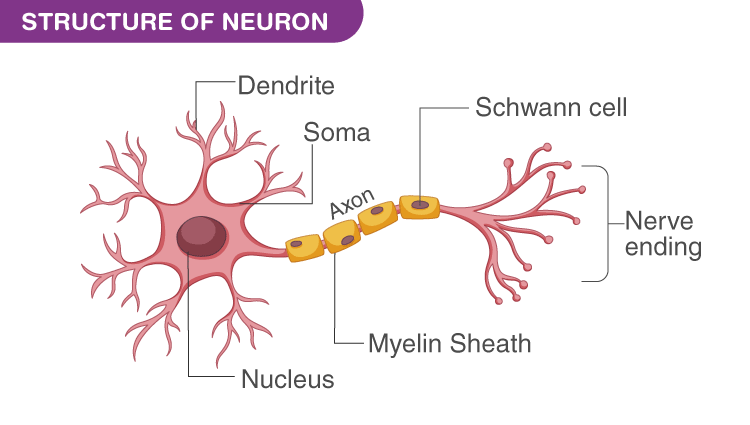
\includegraphics[width=.8\textwidth]{figures/01_neuron.png} 
    \captionof{figure}{General structure of a neuron, including the soma, axon, dendrites, and synaptic terminals. \textit{Image source: \cite{Byjus_Neuron}}}
    \label{fig:neuron_structure}
\end{center}

The soma, or cell body, contains the nucleus and most of the cell’s metabolic machinery. It integrates incoming electrical signals and initiates responses. Extending from the soma is the axon, a long, cable-like projection that transmits electrical impulses away from the neuron. In many cases, axons are insulated by a myelin sheath, which increases the speed and efficiency of signal transmission. The axon terminates in a series of fine branches known as nerve endings, where neurotransmitters are released to communicate with other neurons, muscles, or glands.

Branching in the opposite direction from the soma are the dendrites highly branched extensions that receive incoming signals from other neurons. These inputs are primarily delivered through synapses located on the dendritic surface. The geometry of the dendritic arbor plays a crucial role in determining how information is collected and integrated.

Although these core structures form the basis of neuronal communication, much of the complexity of neural signaling emerges at finer scales. Subtle variations in dendritic branching and microscopic protrusions known as dendritic spines add another layer of computational and biological richness. These features are not only essential for synaptic transmission but are also key to understanding how the brain adapts, learns, and changes with experience.

\subsection{Dendrites}
Dendrites are branched extensions that emerge from the neuronal soma and serve as the primary sites for receiving synaptic input. Their tree-like structure enables neurons to connect with thousands of other cells, forming a base for complex signal integration across neural circuits. The shape and spatial arrangement of the dendritic branching play a central role in how inputs are filtered and relayed towards the soma \cite{Peng_2015}.

Dendritic geometry varies significantly across neuron types. Some neurons exhibit compact, highly branched trees optimized for local connectivity, while others, like pyramidal neurons, extend long apical dendrites that span multiple cortical layers. These morphological variations shape the electrical and computational properties of each neuron \cite{Yuste_2001}. A simplified schematic of dendritic structure is shown in \autoref{fig:dendrite_structure}, highlighting how dendrites emerge from the soma and serve as platforms for synaptic input.

\begin{center}
    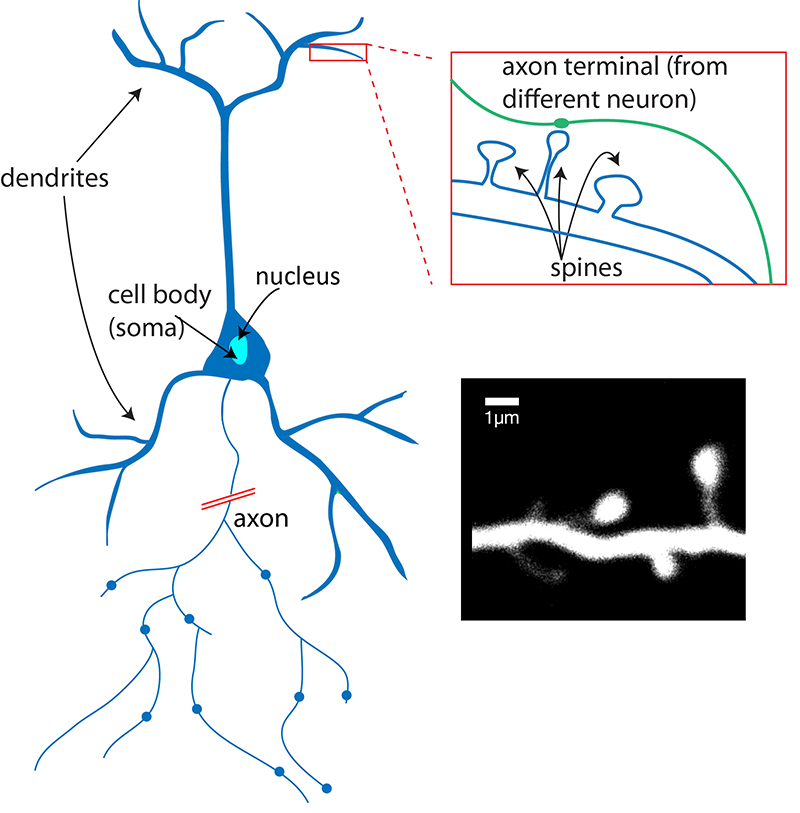
\includegraphics[width=.6\textwidth]{figures/02_dendrite_structure.jpg} 
    \captionof{figure}{A neuron with labeled dendrites, a zoomed-in view of dendritic spines receiving input from an axon terminal and a microscopic image of a dendrite and dendritic spine. \textit{Image source: \cite{dendrite_structure}}}
    \label{fig:dendrite_structure}
\end{center}

In addition to their passive role in collecting signals, dendrites also exhibit active electrical properties. Voltage-gated ion channels along the dendritic membrane can locally amplify or modulate synaptic inputs, allowing for complex forms of signal integration. This transforms dendrites from passive conduits into active computational elements capable of processing input non-linearly before it reaches the soma.

Dendritic structure is also sensitive to developmental cues and environmental changes. Alterations in dendritic length, branching complexity, or arbor orientation have been observed in conditions such as Alzheimer's disease, schizophrenia, and autism spectrum disorders \cite{Frank_2018}. These morphological signatures make dendrites important markers for both healthy function and neuropathology.

The biological complexity of dendrites is clearly visible under high-resolution microscopy. As shown in \autoref{fig:flourocence_image_dendrite}, fluorescence imaging reveals the intricate branching and fine-scale organization of dendritic trees, along with densely distributed spine-like structures emerging along their length.

\begin{center}
    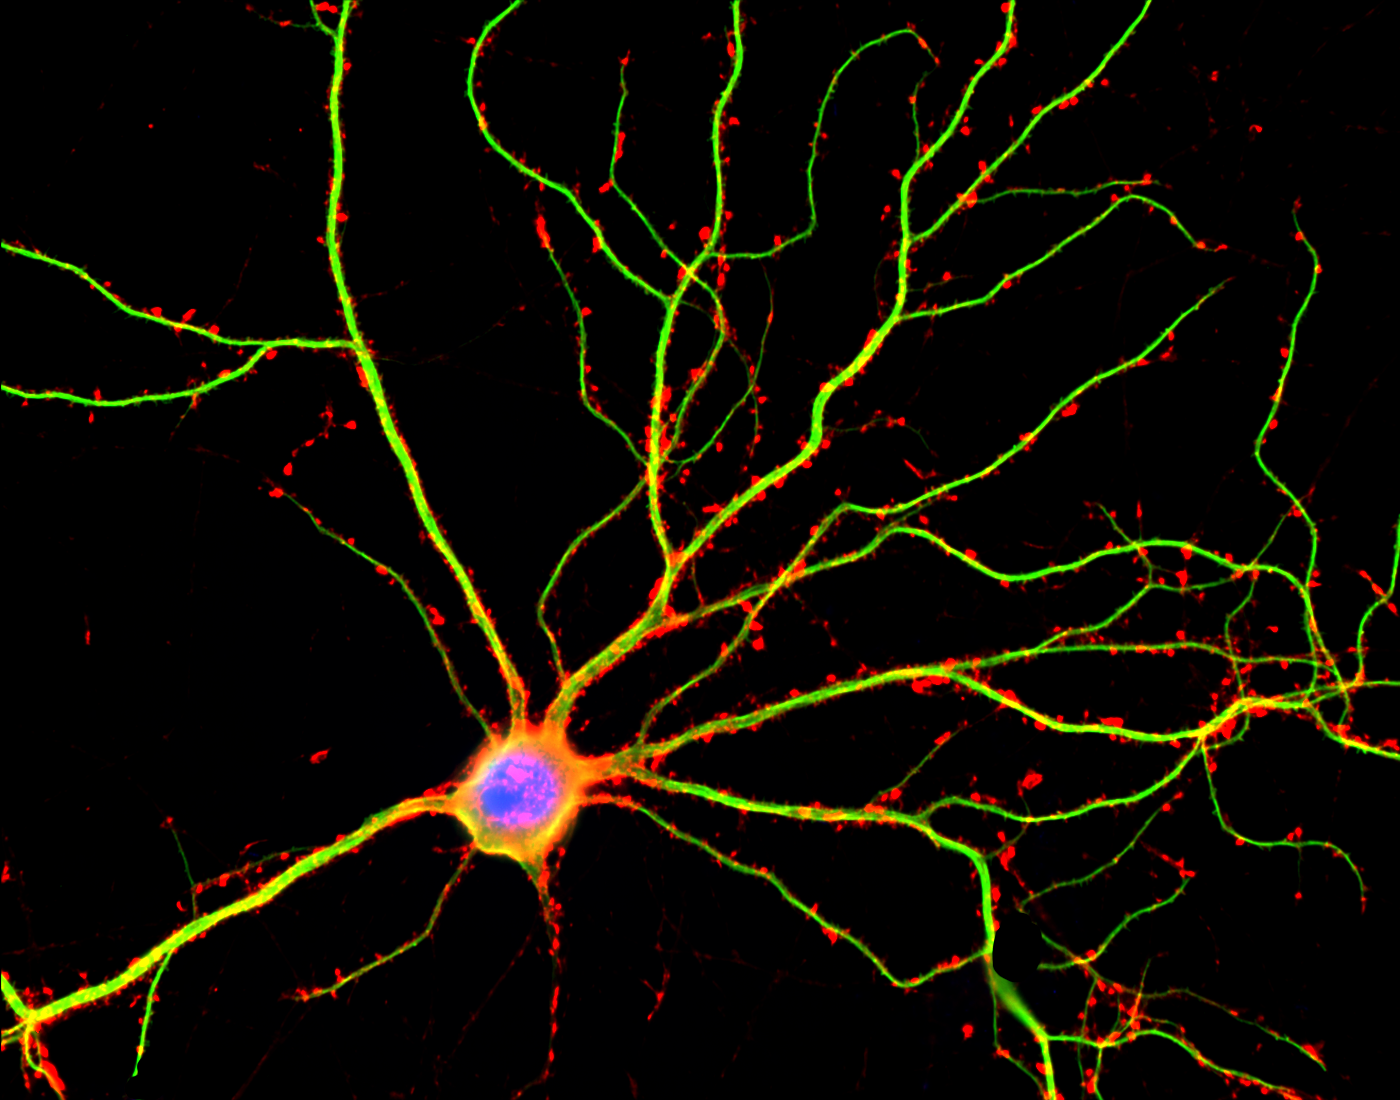
\includegraphics[width=.6\textwidth]{figures/03_flourocence_image_dendrite.png} 
    \captionof{figure}{Fluorescence microscopy image of a neuron showing extensive dendritic branching (green) and spine structures (red) emerging from the dendritic shafts. The soma is labeled in blue. \textit{Image source: \cite{flourocence_image_dendrite}}}
    \label{fig:flourocence_image_dendrite}
\end{center}


These spines, small protrusions that host the postsynaptic structures form the majority of excitatory synapses in the brain and add an additional layer of structural complexity to dendritic processing. 

\subsection{Dendritic Spines}
Dendritic spines are small, membrane-bound protrusions that emerge from dendritic shafts and form the postsynaptic site of most excitatory synapses in the mammalian brain \cite{Yuste_1995}. Each spine typically connects to a single presynaptic axon terminal and functions as a signaling unit. This structural isolation allows spines to regulate calcium dynamics, receptor trafficking, and synaptic strength independently from the parent dendrite \cite{Yuste_2001}.

Although small, often less than one micrometer in diameter; spines exhibit rich morphological detail. They consist of a bulbous spine head connected to the dendritic shaft by a narrow spine neck. The head houses neurotransmitter receptors and postsynaptic scaffolding proteins, while the neck restricts signal diffusion, effectively isolating synaptic activity \cite{Pfeiffer_2018}. This architecture is depicted in \autoref{fig:spine_3d}, which illustrates the spatial relationship between the presynaptic bouton, postsynaptic spine, and dendrite.

\begin{center}
    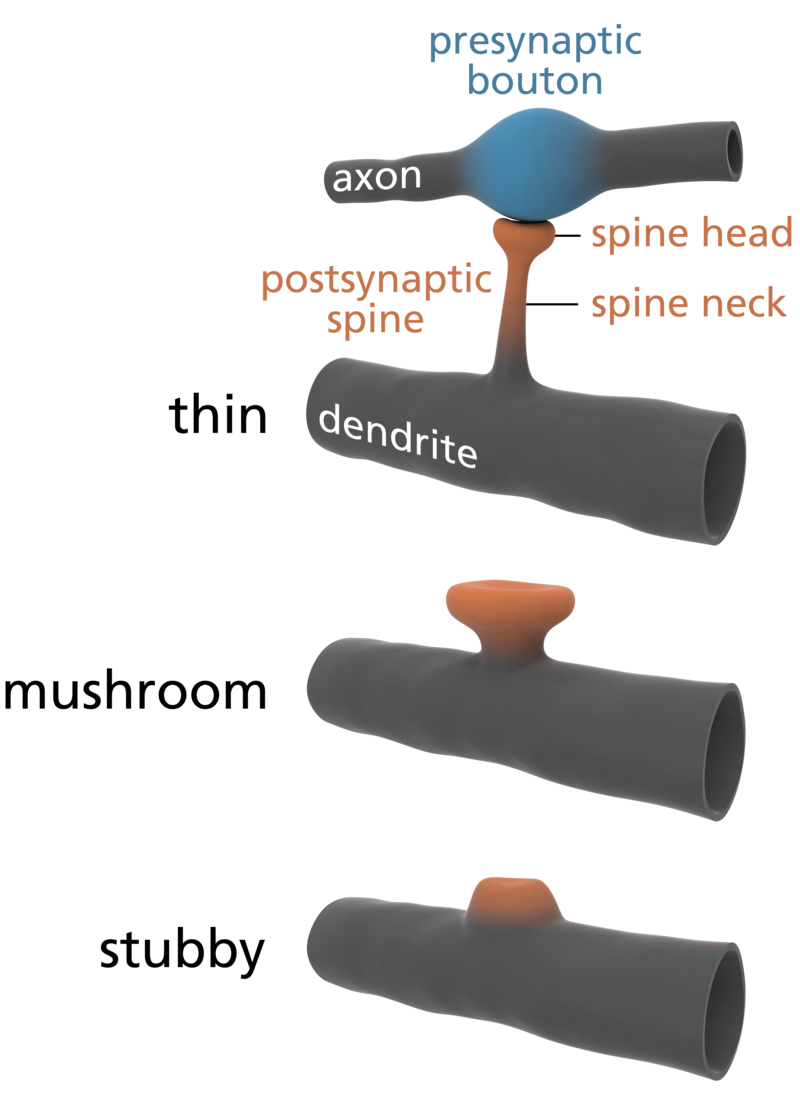
\includegraphics[width=.6\textwidth]{figures/04_spine_3d.png} 
    \captionof{figure}{3D schematic of dendritic spine structure and different spine morphologies including a presynaptic bouton, thin, mushroom and stubby spines. \textit{Image source: \cite{spine_3d}}}
    \label{fig:spine_3d}
\end{center}

Spine morphology is diverse and often reflects functional status. Spines can be long and thin, short and stubby, mushroom-shaped with prominent heads, or in transitional forms. These shape categories are commonly used as indicators of synaptic maturity and stability. Mushroom-shaped spines are considered mature and more stable, while thin or filopodial spines are more dynamic and associated with new or weakly potentiated synapses \cite{Vidaurre_2022}. While this classification is useful, it is inherently qualitative and dependent on imaging resolution and sampling angle.

High-resolution fluorescence microscopy (\autoref{fig:spine_closeup}) reveals that spines are densely distributed along dendritic arbors and vary in spacing and orientation. In practice, their small size and proximity make them difficult to segment and quantify accurately, especially in three-dimensional datasets. The spine neck often falls below the resolution limits of optical systems, and nearby spines can merge or occlude one another. It certainly causes problems for the experts to understand the morphology of the spines.

\begin{center}
    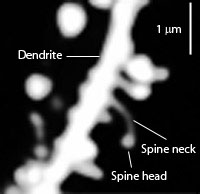
\includegraphics[width=.6\textwidth]{figures/05_spine_closeup.jpg} 
    \captionof{figure}{Image showing the anatomical components of dendritic spines: spine head, neck, and dendritic shaft. \textit{Image source: \cite{spine_3d}}}
    \label{fig:spine_closeup}
\end{center}

Dendritic spines are not only structurally important but also clinically relevant. Similar to the dendrites, abnormalities in spine number, size, or morphology are linked to a variety of neurodevelopmental and neurodegenerative disorders \cite{Rodriguez_2008, Dickstein_2016}. Spines are widely studied as biomarkers of synaptic health and plasticity. Their biological complexity and imaging challenges make dendritic spines a prime target for computational segmentation tools. 

\section{Microscopy for Dendritic Imaging}
Advances in optical microscopy have played a central role in enabling the visualization of dendrites and dendritic spines at submicron resolution, which is essential for understanding synaptic connectivity and plasticity in the brain. Among these, \textit{two-photon laser-scanning microscopy} has become a foundational method in neuroscience for imaging fluorescently labeled neurons deep within scattering tissue.  Its use of near-infrared excitation allows for reduced photodamage and deeper penetration compared to conventional single-photon systems, making it particularly effective for in vivo imaging of dendritic spine dynamics during development, learning, and synaptic remodeling \cite{Pan_2008, Rose_1999}. \textit{Confocal microscopy}, though more limited in imaging depth, remains widely used in fixed tissue and offers high-resolution optical sectioning through pinhole-based light rejection. It is particularly effective when combined with lipophilic dyes or immunostaining protocols for visualizing dendritic cells in both animal and human brain samples \cite{Sun_2024}. More recently, \textit{\gls{STED} microscopy} has enabled super-resolution imaging of live neurons by breaking the diffraction limit through precise spatial depletion of fluorescence. This allows fine structural features such as spine necks, head curvature, and micron-scale protrusions to be resolved at scales below 70 nm, revealing aspects of synaptic architecture that were previously inaccessible with conventional techniques \cite{Nagerl_2008}. These imaging tools not only facilitate visualization, but also support the quantification of spine density, shape, and volume critical for correlating morphological features with synaptic function. Subtypes such as mushroom, stubby, thin, and branched spines can be classified and tracked across time-lapse datasets. Furthermore, combining these modalities with fluorescent labeling strategies, such as Dil stain ballistic tracing or genetically encoded markers, enables large-volume imaging with cellular specificity and structural fidelity \cite{Sun_2024}. Together, these methods provide the biological and anatomical precision required for quantitative modeling and segmentation tasks, forming a crucial foundation for segmentation tasks.

\section{From Microscopy to Morphology: Image Segmentation in Biomedical Imaging}
Microscopy provides high-resolution images of neuronal structures, capturing the complex morphology of dendrites and the fine architecture of dendritic spines. However, these raw images alone are not directly usable for computational analysis. In order to model or quantify neuronal structures, their spatial boundaries must first be extracted from the image domain. This process, known as \textit{segmentation}, involves delineating the foreground structures from the background, producing machine-readable masks that serve as the foundation for automated analysis.

Segmentation refers to the process of assigning a label to each pixel in an image, allowing specific structures to be isolated from their surroundings. In biomedical imaging, this typically involves producing binary or multi-label masks that indicate where particular anatomical or cellular features are located. In contrast to tasks like classification or object detection, segmentation provides precise, pixel-level boundaries, which is essential when working with fine structures such as dendritic shafts or individual spines. These masks can then be used to compute morphometric features, enable automated quantification, or serve as training data for learning-based methods.

Segmentation is a critical step in transforming image data into structured representations that can be analyzed, measured, or modeled computationally. For neuroscience applications, it enables the quantification of dendritic length, branching complexity, and spine density across large datasets \cite{Weaver_2004}. Segmentation also facilitates the construction of ground truth labels for training and evaluating models, making it central to any pipeline that aims to automate morphological analysis \cite{Basu_2018}. Manual annotation, while often considered the gold standard, is time-consuming, subject to annotator bias, and infeasible at scale \cite{Mancuso_2013}.  As datasets have grown in size and complexity, the demand for reliable and reproducible automated segmentation has become increasingly important.

Despite its importance, segmentation in biomedical imaging particularly in neuroscience microscopy remains a challenging task. Dendritic structures can vary greatly in size, shape, and orientation, often appearing as overlapping or densely packed regions in noisy backgrounds. Variability in labeling protocols, microscope settings, and biological tissue further complicates consistent segmentation \cite{Okabe_2020}. Spine structures, in particular, may be faint or partially occluded, requiring highly sensitive algorithms to detect and isolate them accurately \cite{Wang_2015}. 

Before deep learning became prevalent, segmentation in microscopy relied on classical computer vision techniques. These approaches were often effective on carefully controlled datasets but lacked the robustness to handle broader variability without significant manual tuning. Still, these techniques marked the first wave of automation in neuronal image analysis, demonstrating that segmentation could be achieved computationally and forming the methodological foundation for the learning-based techniques that followed. This progression ultimately enables more adaptable Deep Learning based approaches like \gls{DeepD3} or foundation model based approaches like Neuro-\gls{SAM}, to address the demands of modern neuroscience imaging.

\section{Classical Computer Vision for Dendrite and Dendritic Spine Segmentation}
Before the emergence of deep learning based models, the task of segmenting dendrites and dendritic spines was approached using classical computer vision techniques. These methods relied on rule-based algorithms designed to enhance, separate, and refine structural features in microscopy images without the need for large training datasets. In an era when annotated data were scarce and computational resources were limited, classical approaches provided a practical pathway for automating morphology extraction. Though often sensitive to image quality and parameter settings, these techniques formed the first generation of automated pipelines for neuronal structure segmentation, and continue to serve as important components in preprocessing and baseline workflows. Numerous studies have applied variations of these methods to isolate dendritic structures, trace their paths, and detect spines with varying degrees of accuracy \cite{Weaver_2004, Okabe_2020, Erdil_2013}.

\subsection{Emergence of Classical Computer Vision}

Microscopy images often suffer from noise, uneven illumination, and low contrast factors that can obscure fine neuronal structures and degrade segmentation performance. To address these issues, classical computer vision pipelines typically began with preprocessing steps aimed at enhancing image quality. Gaussian filtering was commonly used to reduce high-frequency noise while preserving structural boundaries, and median filtering proved effective at removing salt-and-pepper noise without significantly blurring edges \cite{Marr_1980, Tukey_1977}. Global histogram equalization techniques, as well as more advanced methods like \gls{CLAHE}, were applied to improve contrast and reveal features in images with uneven intensity profiles \cite{Gonzalez_2002, Zuiderveld_1994}. These enhancements were essential for highlighting faint spine structures and thin dendritic shafts. For instance, Weaver et al. \cite{Weaver_2004} employed multiscale smoothing filters to aid morphometric analysis of dendritic arbors, while Roszkowska et al. \cite{Roszkowska_2016} emphasized the role of adaptive contrast enhancement in improving dendritic spine visibility in fluorescence microscopy. These preprocessing techniques were not merely aesthetic improvements; they were necessary to ensure that subsequent segmentation algorithms could operate reliably on noisy or artifact-prone microscopy data. \autoref{fig:preprocessing} shows an example of how preprocessing techniques effectively removes the noise from the microscopic image.

\begin{center}
    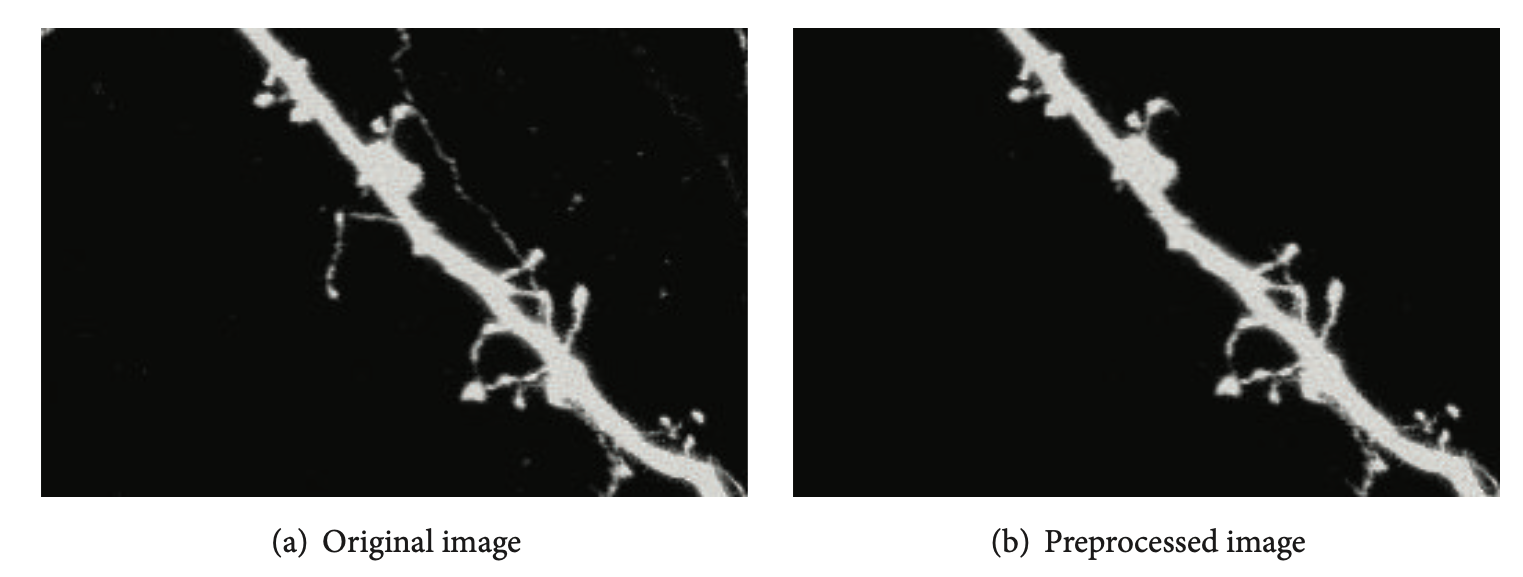
\includegraphics[width=.9\textwidth]{figures/06_preprocessing.png} 
    \captionof{figure}{An example of preprocessing. 2D median filtering was used followed by \gls{PDE} proposed by Wang et el \cite{Wang_2008}. \textit{Image source: \cite{Wang_2015}}}
    \label{fig:preprocessing}
\end{center}


After preprocessing, segmentation pipelines often relied on thresholding to isolate dendritic structures based on intensity. Otsu’s method, which determines a global threshold by minimizing intra-class variance, became one of the most commonly used algorithms for binarizing microscopy images with clear contrast between labeled neurons and background \cite{Otsu_1979}. However, many neural datasets exhibit uneven illumination or local intensity fluctuations, particularly in two-photon or confocal stacks making global thresholds unreliable \cite{Wang_2015}. To address this, researchers turned to adaptive thresholding methods, which compute local thresholds over image patches and offer more resilience to intensity inhomogeneity.

Several studies integrated thresholding with region-based techniques to improve segmentation sensitivity. Weaver et al. \cite{Weaver_2004} used adaptive thresholding followed by structural refinement to extract complex dendritic trees. Roszkowska et al. \cite{Roszkowska_2016} also discussed the utility of adaptive thresholding when applied to high-resolution optical images, noting improved detection of spines in densely labeled samples. Meanwhile, earlier methods such as connected component labeling can also be used as part of a broader segmentation and 3D quantification pipeline \cite{Basu_2018}.

Despite their accessibility and speed, these methods often struggled with ambiguous or overlapping structures and were highly sensitive to parameter tuning. Their performance was closely tied to imaging quality and uniformity, conditions rarely guaranteed across diverse datasets.

\subsection{Morphological Operations and Skeletonization}
Once an initial binary segmentation mask was produced, classical image analysis workflows often relied on \textit{mathematical morphology} to refine neuronal structures prior to measurement. Morphological operations act on the shape of binary objects rather than their intensity, making them especially suited for removing small specks of noise, bridging gaps in dendritic shafts, and ensuring connectivity between spine necks and their parent dendrites. Fundamental operators such as \textit{dilation} and \textit{erosion} were applied to expand or shrink the foreground regions, while compound operations like \textit{opening} (erosion followed by dilation) removed isolated noise, and \textit{closing} (dilation followed by erosion) filled small gaps within processes. \autoref{fig:morphology} shows the working of morphological operations such as Dilation, Erosion, Closing and Opening on an image. In dendritic spine segmentation, these steps were crucial for preserving the fine morphological continuity necessary for accurate quantification \cite{Weaver_2004, Okabe_2020}.

\begin{center}
    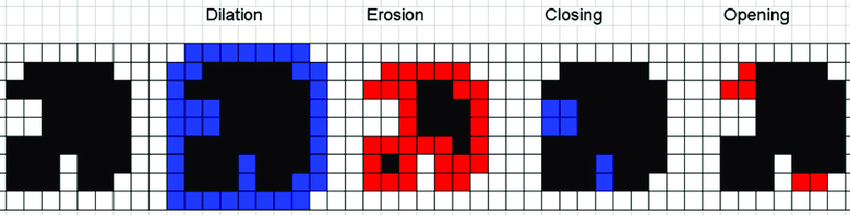
\includegraphics[width=.9\textwidth]{figures/08_morphology.png} 
    \captionof{figure}{Morphological Operations. Black regions represent the original shape, blue regions indicate pixels added during dilation or closing, and red regions indicate pixels removed during erosion or opening. \textit{Image source: \cite{Rutzinger_2011}}}
    \label{fig:morphology}
\end{center}

Several studies in the literature adapted these operations to the anisotropic geometry of neuronal structures. Su et al. \cite{Su_2014} developed a \textit{directional morphological filter} tailored to highlight elongated dendritic shafts while suppressing background interference, which they combined with Hessian-based centerline extraction and shortest path algorithms to trace dendrites and locate spines in 2D projections. In another study, morphological filtering was integrated into a watershed and active contour framework to refine spine boundaries in two-photon images, improving segmentation in cases where spines were closely packed or partially overlapping \cite{Erdil_2013}. Basu et al. \cite{Basu_2018} employed morphological closing in their 3D morphometric analysis to repair fragmented spine necks, ensuring volumetric continuity in reconstructions.

Beyond surface refinement, some pipelines incorporated \textit{skeletonization} to reduce a segmented neuron to its medial axis while preserving connectivity and branch topology. This representation enabled automated measurement of arbor length, branch order, and spatial arrangement of spines. Weaver et al. used skeletonization in combination with graph-based analysis to extract topological features of dendritic trees from 3D reconstructions \cite{Weaver_2004}. In a related approach, researchers enhanced dendritic centerlines using morphological filtering prior to skeletonization, resulting in more stable topology extraction from noisy fluorescence images \cite{Zhang_2016}. Skeleton-based analysis was particularly advantageous when studying branching patterns or reconstructing dendritic paths from large-volume datasets, though it remained sensitive to segmentation noise, small binary artifacts could introduce false branches or disrupt continuity.

While morphological operations and skeletonization formed the backbone of many classical segmentation workflows, their limitations were well recognized. Vigorous morphological filtering could distort delicate anatomical features, altering spine shape or shaft thickness \cite{Roszkowska_2016}. Skeletonization, in turn, often required manual cleaning to remove artifacts, and its parameters such as pruning thresholds were highly dataset dependent. Nevertheless, these methods provided the first scalable, automated tools for structural refinement and topological analysis in dendrite and dendritic spine studies, laying the groundwork for the more adaptive, learning-based segmentation frameworks that followed.

\subsection{Contour and Gradient-Based Methods}
Another important family of segmentation techniques in classical computer vision relies on the detection of object boundaries from changes in image intensity. These \textit{gradient-based methods} locate edges by identifying regions where intensity gradients are high, producing a contour map that can be used to delineate neuronal structures. In microscopy images of dendrites and dendritic spines, such methods were valuable for isolating fine boundaries that thresholding alone could not reliably capture.

Common approaches included the Canny edge detector, which combines Gaussian smoothing to suppress noise with multi-stage gradient analysis to locate thin, well-connected edges, and the Sobel and Laplacian operators, which approximate spatial derivatives of the image \cite{Canny_1986, Sobel_2014, Paris_2011}. While these methods could reveal dendritic shafts and spine perimeters with subpixel precision, their effectiveness depended heavily on preprocessing, as noise or uneven illumination could produce fragmented or false edges \cite{Okabe_2020, Roszkowska_2016}.

To extract complete object boundaries from initial edge maps, \textit{active contour models} (also known as snakes) were widely employed \cite{Kass_1988}. These methods evolve a curve under the influence of internal smoothness constraints and external image forces, allowing the contour to lock onto object edges even when they are irregular or partially missing. Erdil et al. integrated active contours into a hybrid segmentation pipeline for two-photon microscopy images, using them to refine the outlines of dendritic spines after an initial watershed-based separation \cite{Erdil_2013}. The watershed transform, which treats the image as a topographic surface and “floods” it from minima until basins meet at watershed lines, was particularly effective at separating overlapping spines or disentangling dense dendritic regions. Zhang et al. combined directional morphological filtering with watershed segmentation to achieve cleaner separation of closely apposed structures in fluorescence datasets \cite{Zhang_2016}. \autoref{fig:watershed} shows an example of use of watershed algorithm for segmenting a single dendritic spine.

\begin{center}
    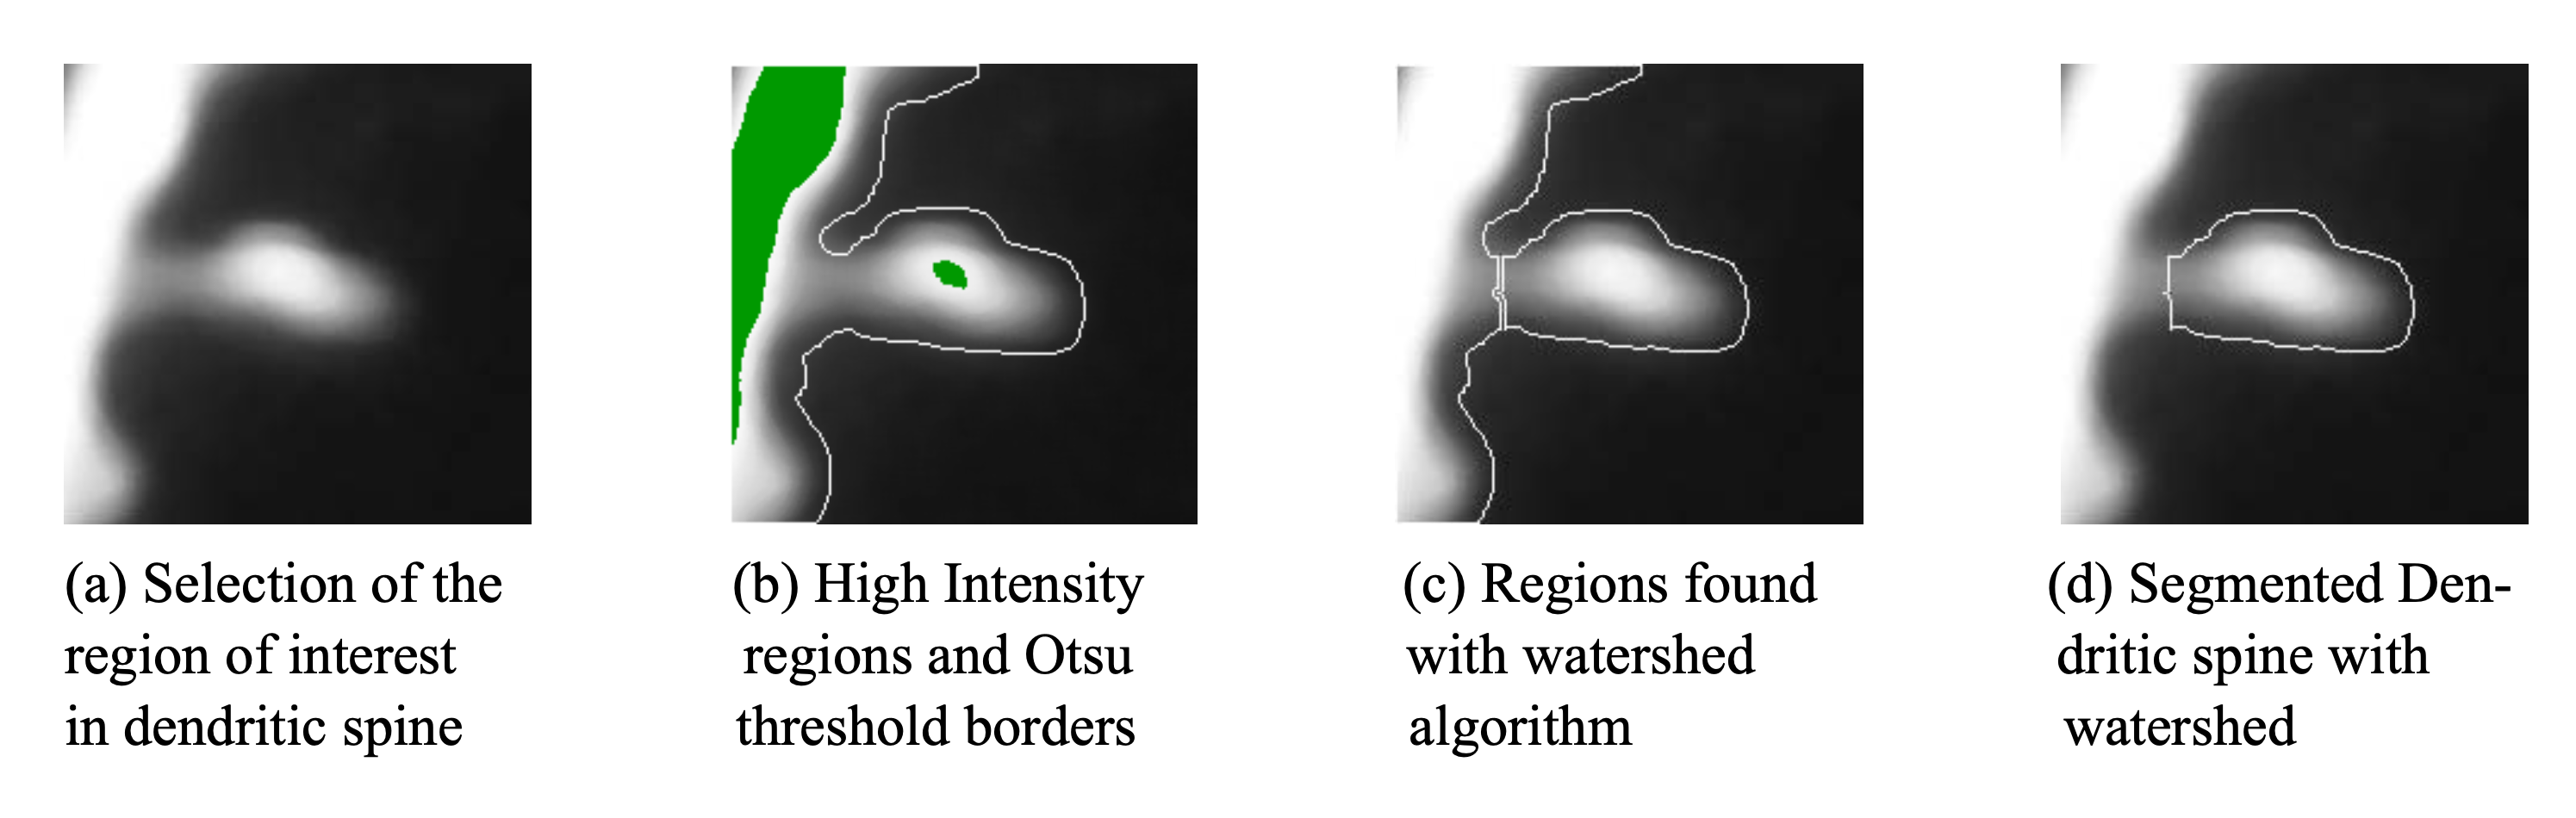
\includegraphics[width=.8\textwidth]{figures/07_watershed.png} 
    \captionof{figure}{Segmentation of a Dendritic Spine with Watershed Algorithm. \textit{Image adapted from: \cite{Erdil_2013}}}
    \label{fig:watershed}
\end{center}

Despite their precision, contour and gradient-based methods are sensitive to weak boundaries, a common occurrence in deep tissue imaging where scattering reduces contrast. They are also prone to over segmentation in the presence of noise, making preprocessing steps such as denoising and contrast enhancement essential. Nonetheless, these methods provided the first automated tools for tracing and refining dendritic boundaries in challenging microscopy datasets, and many concepts from these early algorithms remain embedded in modern learning-based segmentation frameworks.

\subsection{Limitations of Classical Computer Vision}
Classical segmentation methods, while foundational, were highly sensitive to imaging conditions. Thresholding and gradient-based approaches assumed consistent illumination and contrast, yet fluorescence and two-photon microscopy often exhibit depth-dependent attenuation, photobleaching, and uneven staining \cite{Okabe_2020, Roszkowska_2016}. These variations frequently caused fragmented segmentations or missed structures unless parameters were manually adjusted for each dataset.

Parameter dependency was a persistent challenge. Structuring element sizes for morphological filtering, thresholds for edge detection, and active contour parameters typically required dataset-specific tuning \cite{Weaver_2004}. Even minor changes in staining protocols, optical resolution, or imaging depth could necessitate re-optimizing the workflow, limiting reproducibility across laboratories.

Noise and background artifacts further constrained performance. Gradient-based methods often mistook random fluctuations for real boundaries, while excessive denoising risked erasing fine spine structures. Morphological operators and skeletonization could distort delicate features if applied too aggressively, and skeleton-based analyses were especially vulnerable to noise-induced artifacts \cite{Basu_2018, Zhang_2016}.

Ultimately, these methods lacked the adaptability needed to handle the variability of biological data at scale, often requiring extensive human oversight. This inflexibility, coupled with the emergence of large annotated datasets and increased computational power, motivated the shift toward learning-based segmentation approaches capable of capturing complex morphological patterns directly from data.

\section{Deep Learning for Dendritic Segmentation}
The advent of deep learning has transformed the landscape of biomedical image segmentation, offering powerful alternatives to the handcrafted, rule-based methods that previously dominated the field. Unlike classical approaches, which rely on manually engineered filters and carefully tuned parameters, deep learning models learn hierarchical feature representations directly from annotated image data. This ability to capture complex, non-linear relationships between pixel intensities and underlying biological structures has proven especially valuable in neuronal imaging, where dendrites and dendritic spines exhibit high morphological variability, overlap with dense background structures, and often appear under uneven illumination conditions \cite{Weaver_2004, Okabe_2020, Roszkowska_2016}. In particular, \gls{CNN} have enabled pixel-level predictions that are both more accurate and more robust to noise than classical computer vision pipelines \cite{Shea_2015}. Architectures such as U-Net and its derivatives have become the de facto standard for segmentation in microscopy, demonstrating strong performance on diverse datasets, from confocal and two-photon imaging to super-resolution modalities. These advances have made it feasible to automatically extract fine-scale dendritic morphology at scale, accelerating studies of neuronal structure, function, and plasticity \cite{Basu_2018, Fernholz_2024}.

\subsection{Convolutional Neural Networks}
\gls{DNN} are a class of machine learning models composed of multiple layers of interconnected processing units, or neurons, that transform input data into progressively more abstract representations. While fully connected networks, also known as \gls{MLP}, can model complex non-linear relationships, they are inefficient for image data because they treat every pixel as independent and require an impractical number of parameters for high-resolution inputs \cite{Goodfellow_2016}.

\begin{center}
    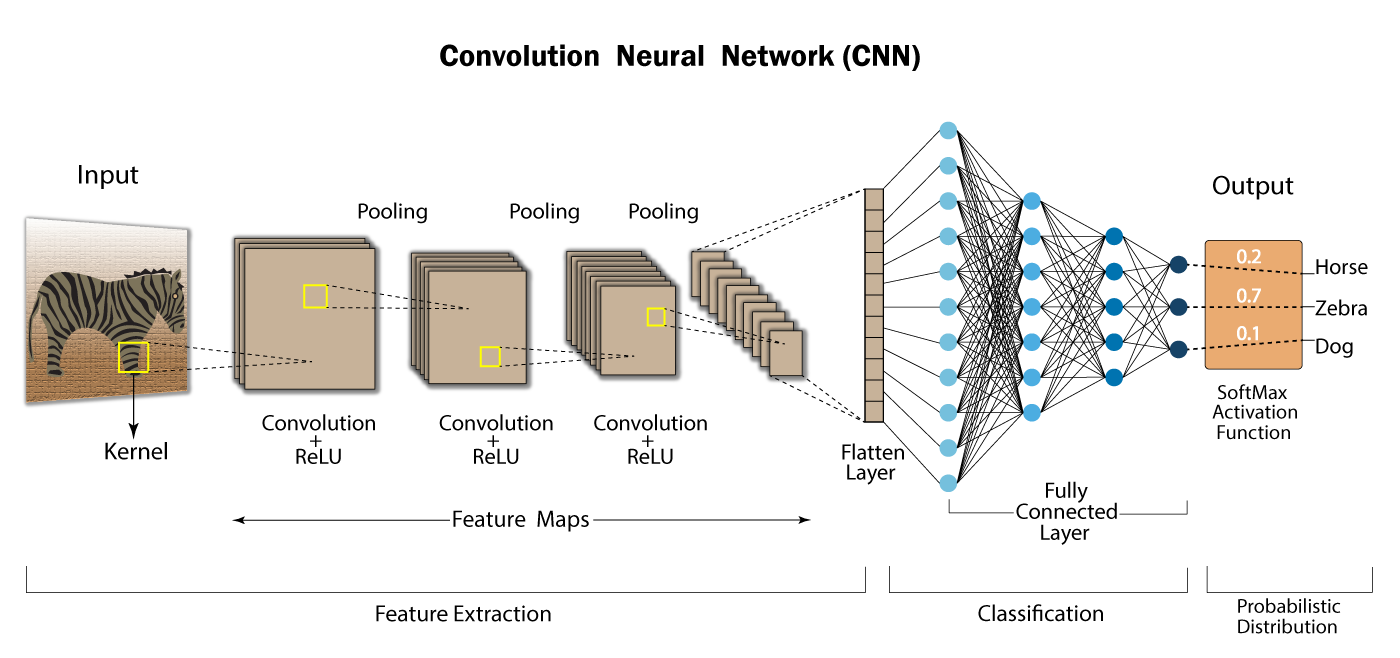
\includegraphics[width=.9\textwidth]{figures/09_cnn.png} 
    \captionof{figure}{Convolutional Neural networks \textit{Image source: \cite{cnn}}}
    \label{fig:cnn}
\end{center}

The \gls{CNN}s address these limitations by introducing convolutional layers, which apply learnable filters across local regions of the input image \cite{LeCun_1989}. An example architecture is illustrated in \autoref{fig:cnn}, where convolutional kernels extract spatial features that are progressively combined to produce a probabilistic classification output. This operation exploits the spatial structure of images, allowing \gls{CNN}s to learn translation-equivariant features such as edges, textures, and shapes through parameter sharing. Pooling layers are often used to progressively reduce spatial resolution while increasing the receptive field, enabling the network to capture both fine details and larger contextual patterns. \gls{CNN}s are also well-suited to biomedical microscopy because their hierarchical feature extraction can detect subtle structural cues such as the elongated geometry of dendrites or the bulbous heads of dendritic spines even in the presence of noise or background clutter \cite{Ronneberger_2015, Falk_2019}.

While \gls{CNN}s were originally developed for image classification, their ability to learn spatial features makes them equally well-suited for dense prediction tasks. Since the widespread success of \gls{CNN}s in computer vision, particularly after the breakthrough performance of AlexNet on ImageNet \cite{Krizhevsky_2012}, these architectures have rapidly become the foundation of most classification and segmentation tasks.
In segmentation, the goal is to assign a class label to each pixel, producing a mask that outlines structures of interest in this case, dendrites and dendritic spines. Most modern segmentation architectures follow an encoder–decoder design: the encoder captures increasingly abstract features through convolution and pooling, while the decoder progressively upsamples and refines these features to recover spatial resolution. The introduction of U-Net in particular marked a turning point, providing a \gls{CNN} design tailored for dense prediction tasks in biomedical imaging and establishing the blueprint for many subsequent architectures in neuronal morphology analysis.

\subsection{Core Architectures}
In deep learning based medical segmentation, a small number of convolutional network designs have emerged as architectural standards, forming the backbone of most modern segmentation pipelines. The most influential among them is the U-Net architecture, introduced by Ronneberger et al. \cite{Ronneberger_2015}, which is a fully convolutional network designed specifically for biomedical image segmentation. As shown in \autoref{fig:unet} the defining feature is a symmetric encoder–decoder structure in which the encoder progressively downsamples the input image through convolution and pooling operations to capture increasingly abstract and context-rich representations, while the decoder upsamples these features to reconstruct a segmentation map at the original resolution. Skip connections link corresponding encoder and decoder stages, allowing high-resolution spatial details lost during downsampling to be directly merged with the upsampled feature maps. This combination of multi-scale context and precise localization makes U-Net particularly well-suited for delineating the fine, elongated shafts of dendrites and the small, bulbous heads of dendritic spines in microscopy images, where both global morphology and minute structural boundaries must be preserved.

\begin{center}
    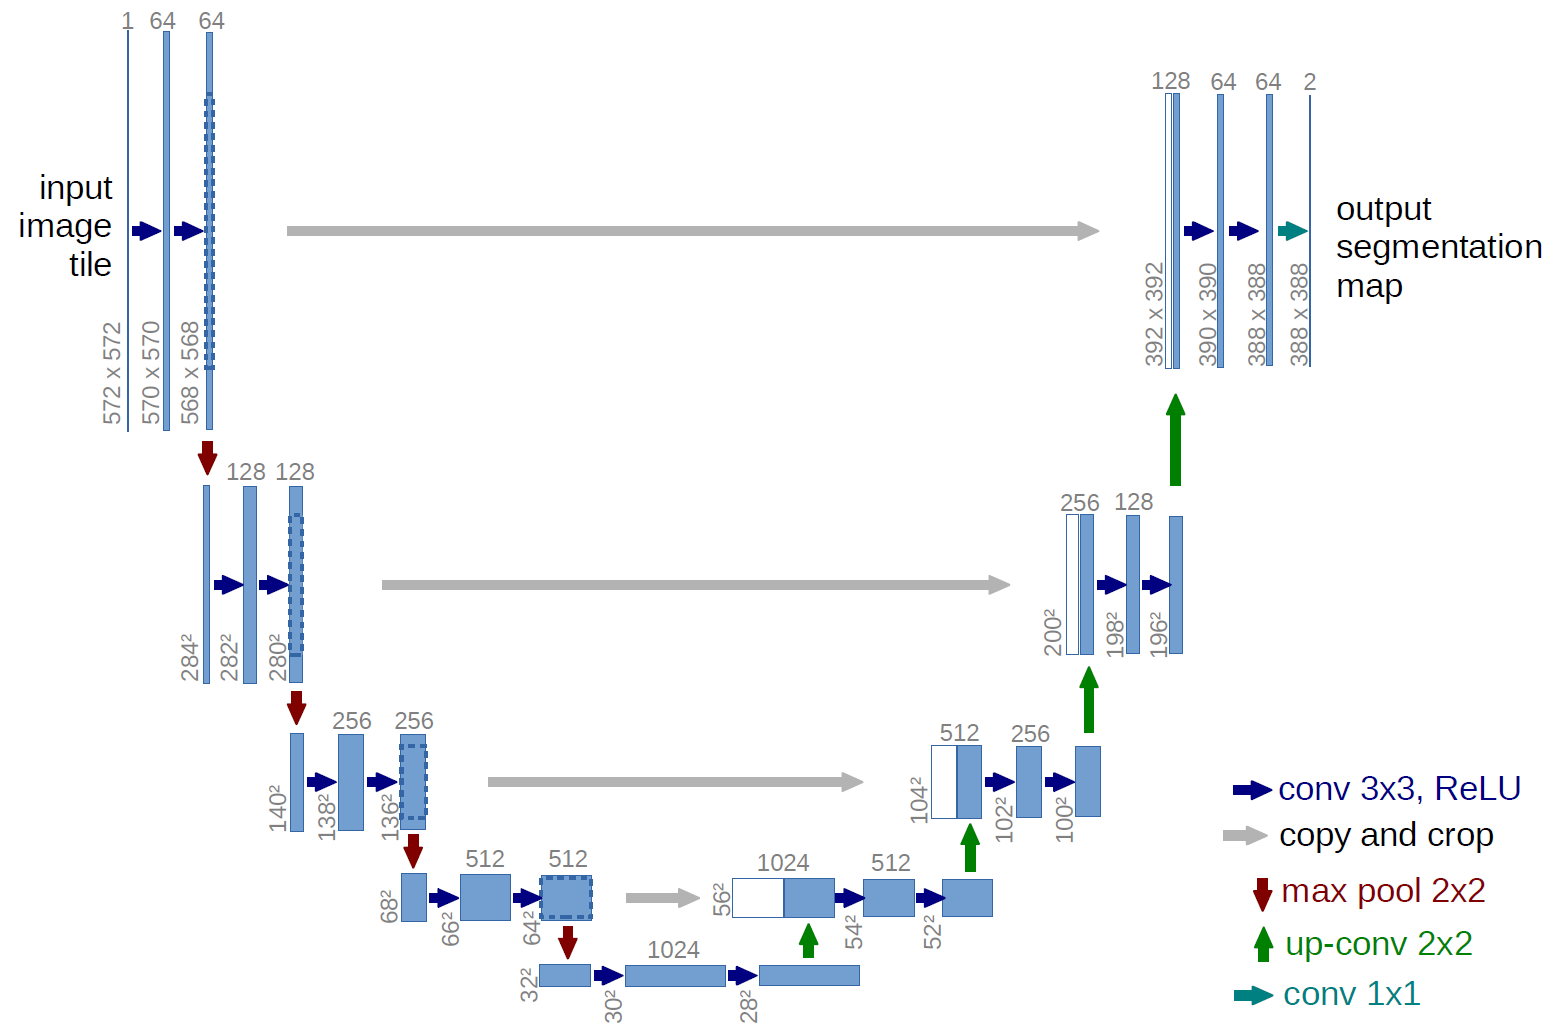
\includegraphics[width=.9\textwidth]{figures/10_unet.png} 
    \captionof{figure}{U-Net Architecture \textit{Image source: \cite{Ronneberger_2015}}}
    \label{fig:unet}
\end{center}

Numerous variants of U-Net have been developed to overcome limitations in biomedical image segmentation, particularly for complex structures such as dendrites and dendritic spines. These adaptations introduce architectural innovations aimed at improving spatial context awareness, gradient propagation, and structural attention. Table~\ref{tab:unet_variants} summarizes key variants relevant to neuronal imaging.


\begin{table}[caption={Summary of U-Net variants relevant to dendritic and spine segmentation}, label=tab:unet_variants]
    \centering
    \begin{tabular}{p{3.2cm} p{3.5cm} p{6.5cm}}
        \toprule
        \textbf{Study / Authors} & \textbf{U-Net Variant} & \textbf{Main Contribution / Novelty} \\
        \midrule
        Çiçek et al. (2016) \cite{Çiçek_2016} & 3D U-Net & Introduced 3D convolutions for volumetric segmentation across z-stacks. \\
        Zhou et al. (2018) \cite{Zhang_2018} & Residual U-Net & Integrated residual connections to support deeper training while preserving fine structure. \\
        Oktay et al. (2018) \cite{Oktay_2018} & Attention U-Net & Added attention gates to focus on spatially relevant features like thin spines. \\
        \bottomrule
    \end{tabular}
\end{table}



% Numerous variants of U-Net have been developed to address specific challenges in biomedical image segmentation, including those encountered in dendrite and dendritic spine analysis. \textit{Three-dimensional U-Net} architectures extend the original design to volumetric data, replacing 2D operations with 3D convolutions to capture spatial context across image stacks. This adaptation has proven effective for segmenting dendritic structures in confocal and two-photon microscopy volumes, where structures span multiple z-planes and continuity between slices is essential for accurate reconstruction \cite{Singh_2017, Vidaurre_2022}. \textit{Residual U-Net} variants integrate residual connections within the convolutional blocks, improving gradient flow during training and enabling the use of deeper models without degradation in performance \cite{Xiao_2018}. Such designs are particularly advantageous when working with high-resolution images where fine structural details must be retained across many processing layers. \textit{Attention U-Net} introduces attention gates that learn to weight spatial features according to their relevance for the segmentation task, helping the network focus on subtle morphological cues such as thin spine necks against cluttered backgrounds \cite{Oktay_2018}. These modifications maintain the core encoder–decoder structure and skip connections of U-Net while enhancing performance for specific data modalities and structural complexities common in neuronal imaging.

\subsection{Applications in Dendritic Segmentation}
U-Net and its derivatives have been widely adopted in frameworks targeting dendrite and dendritic spine segmentation, often serving as the backbone for specialized pipelines. Singh et al. employed a 3D U-Net to segment dendritic arbors from volumetric two-photon datasets, integrating customized loss functions to account for severe class imbalance between neuronal structures and background \cite{Singh_2017}. Vidaurre-Gallart et al. adapted U-Net for high-resolution confocal imaging, introducing patch-based training to handle large image sizes while preserving the context necessary for accurate spine detection \cite{Vidaurre_2022}. Xiao et al. incorporated residual U-Net blocks into a semi-supervised segmentation approach, enabling robust delineation of dendrites in noisy datasets with limited annotations \cite{Xiao_2018}. Several pipelines in the literature combine U-Net feature extraction with post-processing stages such as morphological filtering or skeletonization to refine predictions into biologically interpretable structures, ensuring continuity in dendritic shafts and accurate isolation of individual spines. These adaptations highlight the flexibility of the U-Net architecture, allowing researchers to tailor it to the diverse imaging modalities, resolutions, and labeling conditions encountered in neuroscience.

A prominent recent example of a U-Net inspired framework for dendritic segmentation is \textit{\gls{DeepD3}} \cite{Fernholz_2024}, which was specifically designed for automated detection and quantification of dendrites and dendritic spines across diverse microscopy modalities. \gls{DeepD3} employs a dual-decoder architecture branching from a shared encoder, enabling simultaneous prediction of dendritic shaft and spine masks from the same latent representation. The encoder is a residual \gls{CNN} that enhances gradient flow and supports deeper feature hierarchies, while skip connections preserve high-resolution spatial information. In contrast to the transposed convolutions used in the original U-Net, \gls{DeepD3} uses bilinear upsampling followed by convolution in the decoder stages, reducing checkerboard artifacts and improving the smoothness of predicted boundaries. Batch normalization and the \gls{SiLU} are applied throughout to stabilize training and enhance feature nonlinearity. By training on a large, heterogeneous dataset including confocal, two-photon, and super-resolution images from multiple laboratories \gls{DeepD3} demonstrated strong cross-domain generalization, outperforming single-modality models in both spine detection and dendritic shaft segmentation. This design illustrates how tailoring a U-Net backbone to the morphological characteristics of neuronal structures, combined with broad dataset diversity, can yield robust, scalable segmentation tools for neuroscience.


\subsection{Limitations of Deep Learning based models}
Despite their success, U-Net based architectures and their variants face limitations when applied to dendrite and dendritic spine segmentation. Their performance often depends heavily on the quality and quantity of annotated training data, which in neuroscience is labor-intensive to produce and prone to inter-annotator variability \cite{Okabe_2020}. Models trained on a single modality or dataset can exhibit reduced generalization when confronted with differences in imaging resolution, contrast, or labeling protocols \cite{Roszkowska_2016}. Even architectures designed for cross-domain performance, such as \gls{DeepD3}, may underperform on data with imaging artifacts or morphological patterns not represented in the training set. Additionally, while U-Net’s skip connections preserve fine details, they can also propagate noise or background clutter into the final segmentation, leading to false-positive detections, particularly problematic for small embedded spines. The memory footprint and computational cost of 3D variants further restrict their use in large volumetric datasets without access to high-performance hardware. These constraints highlight the need for models that can generalize beyond the distribution of their training data, adapt to novel imaging conditions, and operate effectively with limited or imperfect annotations.

These limitations have motivated a shift toward more generalizable and adaptable segmentation approaches, culminating in the recent exploration of \textit{foundation models} for biomedical imaging. Unlike task-specific \gls{CNN}s that must be trained from scratch for each dataset or imaging modality, foundation models are pretrained on large, diverse image collections and can be adapted to a wide range of segmentation tasks through fine-tuning or prompt-based interaction. In the context of dendrite and dendritic spine segmentation, such models hold the promise of robust performance across different microscopes, staining methods, and species without the need for extensive retraining. This paradigm shift offers a path toward overcoming the constraints of conventional architectures like U-Net and \gls{DeepD3}, paving the way for tools such as Neuro-\gls{SAM} that leverage the representational power of foundation models to deliver interactive, high-resolution, and biologically meaningful segmentation.

\section{Foundation Models for Dendritic Segmentation}
Deep learning has transformed dendritic segmentation over the past decade, yet even the most advanced \gls{CNN}-based architectures remain limited by their dependence on task-specific training and narrow domain generalization. Foundation models promise to break through these constraints. Trained on vast and diverse datasets, they learn general-purpose visual representations that can be adapted to new segmentation tasks with minimal additional data. For neuroscience, this opens the possibility of accurately segmenting dendrites and spines across imaging modalities, species, and experimental conditions without exhaustive retraining. The following subsections explore the principles behind foundation models, their architectures, and their potential to redefine automated neuronal image analysis.

\subsection{Foundation Models}
Foundation models are large-scale, pretrained neural networks designed to learn general-purpose representations from massive and diverse datasets \cite{Bommasani_2021}. Unlike task-specific models that are trained from scratch for a single objective, foundation models can be adapted to a wide variety of downstream tasks often with minimal fine-tuning or through prompt-based interaction. This versatility arises from their training paradigm: pretraining on billions of images or image-text pairs enables the model to learn robust, semantically rich feature representations that extend far beyond the scope of the original training data.

A key driver behind the rise of foundation models in computer vision is the transformer architecture, originally developed for natural language processing but later adapted to images in the \gls{ViT} \cite{Vaswani_2017, Dosovitskiy_2020}. The standard transformer architecture, consisting of stacked self-attention and feed-forward layers with residual connections is illustrated in \autoref{fig:transformer}. Transformers replace the fixed-size receptive fields of \gls{CNN}s with self-attention mechanisms, which allow every token (or image patch) to attend to every other. This global context modeling enables them to capture long-range dependencies an especially important property for dendritic segmentation, where local features such as spine necks must be interpreted in the context of the surrounding dendritic structure. Transformers also offer greater architectural flexibility, as they are not bound to the locality constraints and inductive biases of convolutions, which can limit generalization across domains.

\begin{center}
    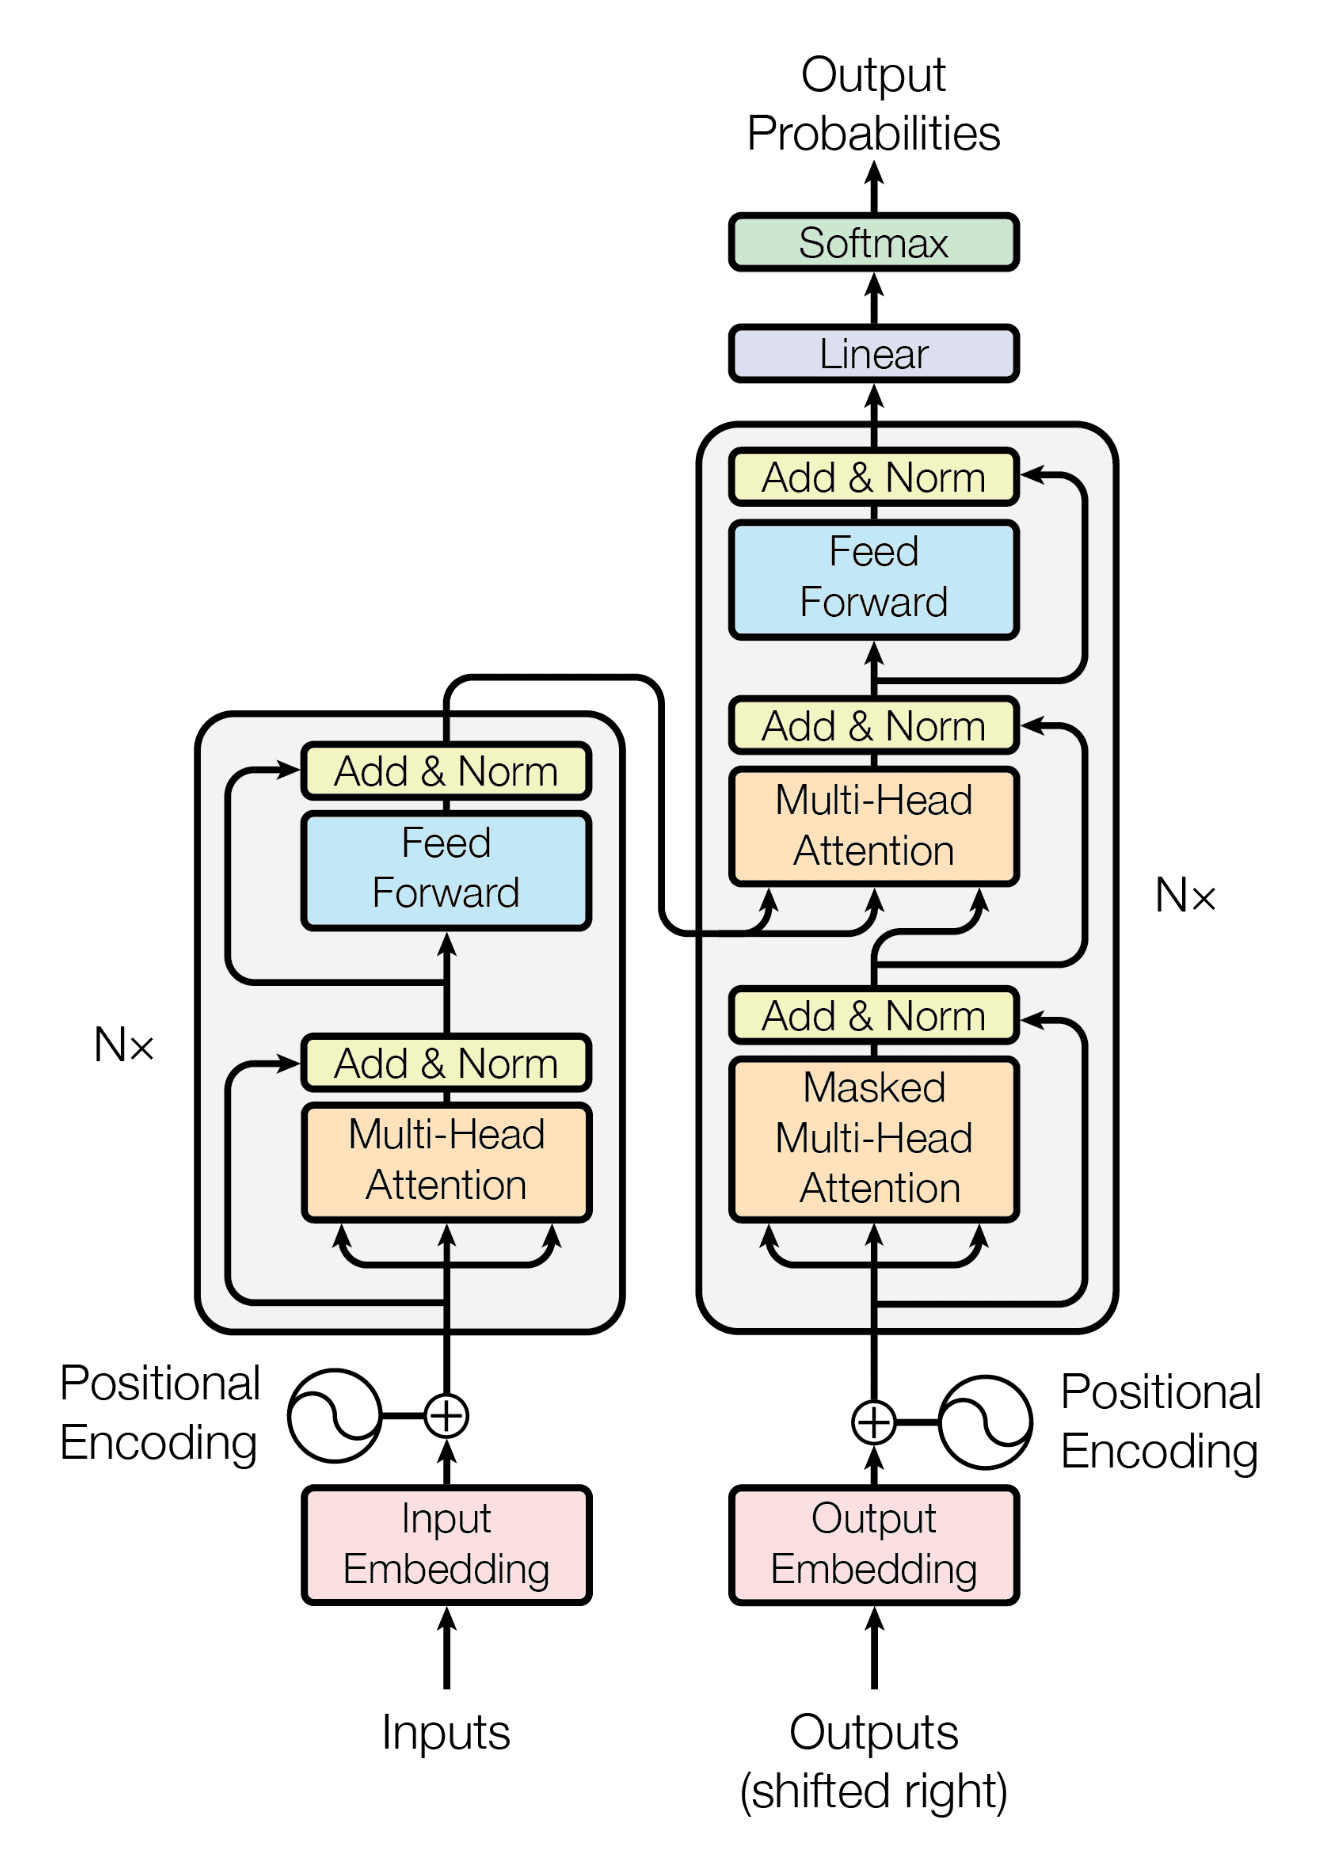
\includegraphics[width=.7\textwidth]{figures/11_transformer.png} 
    \captionof{figure}{Transformer Architecture \textit{Image source: \cite{Vaswani_2017}}}
    \label{fig:transformer}
\end{center}

Compared to traditional \gls{CNN}-based architectures like U-Net, foundation models offer several advantages for biomedical imaging. First, they require fewer domain-specific adjustments when transferring to a new modality or imaging protocol, reducing the time and computational cost of model adaptation. Second, their global attention mechanisms can help disambiguate faint, low-contrast structures in complex backgrounds, conditions common in neuronal microscopy. Third, pretraining on diverse datasets mitigates overfitting to the limited annotated data typically available in neuroscience \cite{Okabe_2020}. These properties make foundation models an attractive candidate for dendrite and dendritic spine segmentation, where robustness across scales, modalities, and labeling conditions is critical for reproducibility and scalability.


\subsection{Key Vision Foundation Models}
\gls{ViT} marked a major shift in computer vision by applying the transformer architecture originally developed for sequential data in natural language processing to images \cite{Dosovitskiy_2020}. \gls{ViT} divides an image into fixed-size patches, linearly embeds each patch, and processes the sequence of embeddings through multiple layers of multi-head self-attention and feed-forward networks. This design allows the model to capture long-range dependencies between image regions without the locality constraints of convolutional kernels. Despite requiring substantial training data to achieve competitive performance, ViT demonstrated that transformers could match or surpass convolutional networks on large-scale vision benchmarks, inspiring a new generation of vision backbones.

Subsequent models refined the \gls{ViT} architecture to improve efficiency and data requirements. The Swin Transformer introduced a hierarchical structure with shifted window attention, reducing computational complexity while enabling multi-scale feature extraction \cite{Liu_2021}. \gls{DeiT} employed knowledge distillation \cite{Hinton_2015} and optimized training strategies to make transformer training feasible on smaller datasets \cite{Touvron_2021}. These innovations paved the way for transformer-based models to be used as universal backbones across diverse vision tasks, including detection, classification, and segmentation.

In biomedical imaging, transformer-based backbones have shown promise for segmentation tasks requiring both local precision and global context. Their self-attention mechanisms can help disambiguate fine structures such as thin spine necks when surrounded by complex neuropil, and their global receptive fields make them well-suited to capturing the full morphology of dendritic trees. This convergence of capacity, flexibility, and contextual reasoning set the stage for foundation models like the \gls{SAM} model, which leverage large-scale pretraining and interactive segmentation capabilities to further expand the possibilities for neuronal image analysis \cite{Kirillov_2023}.

\subsection{Segment Anything Model}
\gls{SAM} represents a significant milestone in vision foundation models by introducing a promptable segmentation framework capable of generalizing to previously unseen domains without task-specific retraining \cite{Kirillov_2023}. \gls{SAM} is composed of three primary components: an image encoder, a prompt encoder, and a mask decoder. The image encoder is based on the \gls{ViT}-H) that transforms an input image into a dense embedding map. Here, an embedding refers to a high-dimensional representation that captures the semantic and structural information of the image in a compact numerical form \cite{Frome_2013}. The prompt encoder embeds user-provided prompts such as points, bounding boxes, or free-form text into the same feature space as the image embedding. These two streams are fused in the mask decoder, which outputs one or more candidate masks, each accompanied by a confidence score. The architecture of \gls{SAM} is illustrated in \autoref{fig:sam_architecture} \cite{Kirillov_2023}, which shows the flow from image encoding to mask generation.

\begin{center}
    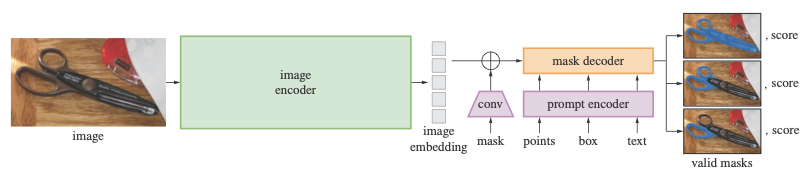
\includegraphics[width=0.95\textwidth]{figures/12_SAM.png} 
    \captionof{figure}{Architecture of the \gls{SAM} model. \textit{Image source: \cite{Kirillov_2023}}}
    \label{fig:sam_architecture}
\end{center}


The model’s pretraining on the SA-1B dataset \cite{SA1B_2023}, which contains over 11 million images of locations, objects, and scenes and 1.1 billion high-quality masks, is central to its ability to generalize across image distributions. This scale of data ensures exposure to a vast diversity of visual concepts, object shapes, and background conditions, enabling \gls{SAM} to handle segmentation tasks far beyond the scope of its training labels. In practice, \gls{SAM} can operate in a zero-shot mode, producing accurate masks for novel objects without fine-tuning. It also supports interactive segmentation: users can iteratively refine results by adding or removing prompts, making it well-suited to workflows where high precision is required with minimal annotation effort.

For biomedical imaging, and particularly dendritic segmentation, \gls{SAM}’s combination of large-scale pretraining and prompt-based flexibility is promising. Its global attention mechanisms can capture extended neuronal structures, while prompt guidance can help isolate fine structures such as spine necks from complex backgrounds. Moreover, its modular design, separating feature extraction from mask prediction makes it possible to adapt the model for domain-specific data without retraining the entire architecture, for example by fine-tuning the prompt encoder or incorporating specialized decoders. 

\subsection{SAM Variants}
Since its introduction, the \gls{SAM} model has inspired a series of adaptations aimed at improving efficiency, domain specialization, and performance in specific imaging contexts. In biomedical imaging, these variants modify either the training strategy or architectural components of \gls{SAM} to better capture small-scale structures, handle limited annotations, and adapt to modality-specific characteristics.

\textit{\gls{SAM} + \gls{LoRA}} \cite{Hu_2021} integrates trainable low-rank matrices into the attention layers of \gls{SAM}’s transformer blocks, enabling parameter-efficient fine-tuning without modifying the full set of pretrained weights. This approach greatly reduces \gls{GPU} memory requirements, making it feasible to adapt \gls{SAM} to high-resolution biomedical data on limited hardware. In microscopy-based segmentation, \gls{SAM} + \gls{LoRA} can leverage the model’s pretrained visual representations while selectively specializing to morphological patterns found in dendrites and dendritic spines.

\textit{Med\gls{SAM}} \cite{Ma_2024} adapts the \gls{SAM} model for medical and biomedical imaging by fine-tuning on a curated collection of domain-specific datasets covering modalities such as \gls{MRI}, \gls{CT}, ultrasound, histopathology, and fluorescence microscopy. This fine-tuning process modifies \gls{SAM}’s pretrained weights to better capture modality-specific textures, noise patterns, and contrast profiles that differ substantially from natural images. In contrast to full retraining, Med\gls{SAM} retains the generalizable feature representations learned during large-scale pretraining while selectively adapting to the statistical characteristics of medical images. Furthermore, Med\gls{SAM} has been shown to outperform vanilla \gls{SAM} in several cross-modality segmentation benchmarks, highlighting the importance of domain adaptation even for powerful foundation models.

\textit{MicroSAM} \cite{Archit_2025} is a microscopy-focused adaptation of the \gls{SAM} model designed to achieve high accuracy in segmenting small structures in dense biological images. It integrates \gls{SAM}’s transformer-based encoder-decoder backbone with multi-scale feature refinement and domain-specific augmentation strategies tailored for microscopy datasets. Unlike the generic \gls{SAM}, which is trained primarily on natural images, MicroSAM incorporates training data and augmentation schemes that better capture the visual characteristics of cellular and subcellular structures. This makes it particularly effective for identifying fine-scale neuronal features, such as dendritic spines, that may be only a few pixels wide in high-magnification images. The approach also includes instance segmentation capabilities optimized for small-object detection, ensuring precise separation of closely packed morphological elements. By combining SAM’s generalization ability with microscopy-specific enhancements, Micro\gls{SAM} bridges the gap between large-scale foundation model pretraining and the demands of high-resolution neuroanatomical segmentation.

The \textit{Segment Anything Model 2} extends the original \gls{SAM} framework with a memory-augmented architecture designed to handle sequential and multi-frame inputs \cite{Ravi_2024}. This is particularly advantageous for volumetric microscopy stacks and time-series imaging, where context from preceding and subsequent frames can disambiguate faint or occluded structures. \gls{SAMv2} retains the modular three-part design, image encoder, prompt encoder, and mask decoder, but introduces two major innovations:

\begin{enumerate}
    \item \textbf{Memory Attention Module}: Positioned between the image encoder and mask decoder, this module enables the model to attend to a temporal or volumetric ``memory bank'' of previously processed frames or slices. This allows \gls{SAMv2} to incorporate contextual cues from neighboring planes in a z-stack or earlier frames in a time-lapse sequence, improving continuity in thin structures like dendritic shafts.

    \item \textbf{Memory Encoder and Bank}:  \gls{SAMv2} maintains a compressed representation of prior frame embeddings in a dedicated memory bank. The memory encoder updates this bank as new frames are processed, creating a persistent context that helps the model maintain segmentation consistency across frames.
\end{enumerate}

These changes address one of the major limitations of the original \gls{SAM}: its inability to exploit temporal or cross-slice correlations. For dendritic segmentation, where fine branches may disappear or fade in individual frames due to imaging noise or depth attenuation, the memory mechanism helps preserve structural coherence. The refined mask decoder in \gls{SAMv2} further improves prompt integration, ensuring that point- or box-based guidance aligns consistently with the target morphology across multiple frames. The architecture of \gls{SAMv2} is illustrated in \autoref{fig:samv2_architecture}, highlighting the addition of the memory attention pathway and the memory bank for contextual information retention.

\begin{center}
    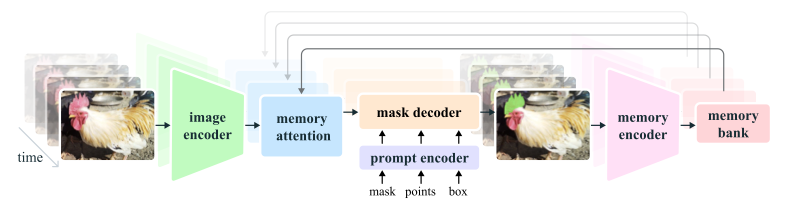
\includegraphics[width=.9\textwidth]{figures/13_SAM2.png} 
    \captionof{figure}{Architecture of the \gls{SAMv2} model \textit{Image source: \cite{Ravi_2024}}}
    \label{fig:samv2_architecture}
\end{center}

\subsection{Relevance to Dendritic Segmentation}
The challenges of dendrite and dendritic spine segmentation such as extreme morphological variability, small structure size, low contrast, and heterogeneous imaging conditions make the problem an ideal candidate for foundation model-based approaches. Unlike traditional \gls{CNN} architectures, which must be trained from scratch or extensively fine-tuned for each dataset, foundation models like \gls{SAM} and its variants offer strong zero-shot performance, rapid adaptability to new domains, and the flexibility to incorporate user guidance through prompts.

In particular, MedSAM brings the benefits of domain adaptation, refining \gls{SAM}’s representations to better handle the textures, contrast profiles, and noise patterns of biomedical imaging. MicroSAM focuses on fine-grained detail recovery in microscopy, making it well-suited for detecting spines that occupy only a few pixels. \gls{SAMv2} extends these capabilities with temporal and volumetric context via its memory attention mechanism, directly addressing the problem of fragmented dendritic reconstructions in 3D stacks or time-lapse sequences. Parameter-efficient tuning strategies such as \gls{SAM} + \gls{LoRA} make it feasible to adapt large foundation models to specialized neuroscience datasets without requiring the computational resources needed for full-model retraining.

Together, these developments offer a compelling path forward for automated neuronal morphology analysis. By merging large-scale pretrained representations with domain-specific enhancements and efficient adaptation strategies, foundation models have shown the ability to deliver high-resolution, biologically faithful segmentations even under challenging imaging conditions. The capacity to generalize across modalities while preserving the ability to detect the finest morphological details signals a major shift in how computational neuroscience approaches dendrite and dendritic spine segmentation.

This convergence of generalization, adaptability, and fine-structure sensitivity forms the conceptual and technical foundation for Neuro-\gls{SAM}. In the following chapter, we build on this background to introduce an interactive, \gls{SAMv2}-based framework designed specifically for dendrite path tracing, dendritic shaft segmentation, spine detection and spine segmentation. By combining the architectural strengths of modern foundation models with domain-tailored refinements, Neuro-\gls{SAM} aims to bridge the gap between state-of-the-art computer vision and the practical demands of high-resolution neuroanatomical analysis.

        \chapter{Methodologies}

The accurate segmentation of dendrites and dendritic spines remains a central challenge in computational neuroanatomy. While recent advances in deep learning have yielded promising automated solutions, these methods often lack the flexibility and interactive control required to address the variability in imaging modalities, experimental conditions, and morphological complexity encountered in real-world neuroscience research. In this chapter, we present a systematic exploration of multiple \gls{SAM}-based architectures beginning with the original \gls{SAM} model, extending to parameter-efficient fine-tuning via \gls{LoRA}, and advancing to the temporally consistent \gls{SAMv2} before introducing our own Neuro-\gls{SAM} framework. Unlike prior fully automated approaches, Neuro-\gls{SAM} is an interactive, modular pipeline that unifies dendrite path tracing, dendrite segmentation, spine detection, and spine segmentation, enabling researchers to move seamlessly from raw volumetric imaging data to high-fidelity morphological reconstructions. Through this progression, we investigate how each methodological step contributes to accuracy, generalization, and annotation efficiency, culminating in a framework designed to answer our central research question.

\section{Data and Preprocessing}
The datasets used in this work were derived from the \gls{DeepD3} dataset \cite{Fernholz_2024}, an in-house curated collection of expert-annotated 3D microscopy image stacks capturing dendritic shafts and dendritic spines under varied imaging conditions. Each stack was manually annotated by three independent experts at single-pixel precision to mitigate annotator bias and promote generalization. Annotations encompassed both dendrites and dendritic spines, providing paired binary masks suitable for supervised segmentation. 

The datasets were designed to address one of the central challenges in neuronal morphology analysis: the extreme variability in imaging modalities, acquisition parameters, and biological structures. By incorporating data from multiple sources and experimental paradigms, this dataset enables the development of segmentation models that generalize beyond a single laboratory or imaging setup. The Table \ref{fig:dataset_description} shows the heterogeneity of imaging conditions for the training, validation and the benchmark dataset. This diversity was intentionally curated to force models to handle variations in spatial resolution, signal-to-noise ratio, and labeling characteristics.

\begin{center}
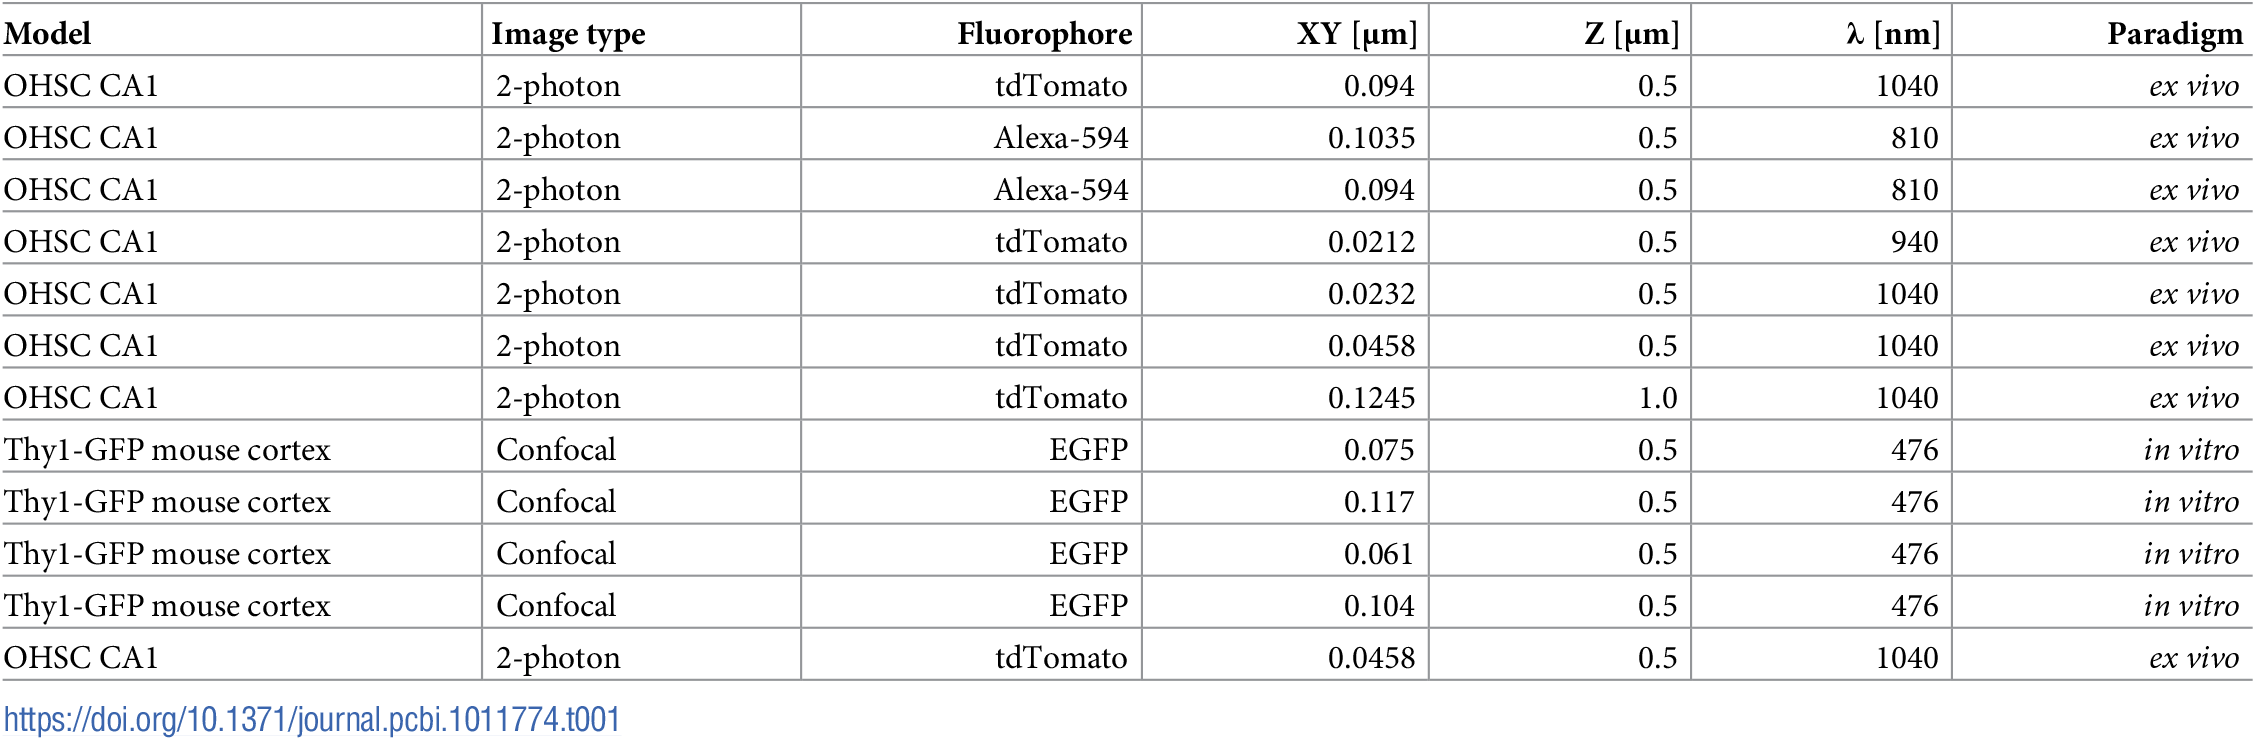
\includegraphics[width=0.95\textwidth]{figures/56_dataset_description.png}
\captionof{figure}{Overview of data (acquired from \cite{Fernholz_2024}), including model organism, brain region, microscopy type, resolution, and imaging wavelength ($\lambda$). Image source: \cite{Fernholz_2024}}
\label{fig:dataset_description}
\end{center}

% \subsubsection{\textbf{Heterogeneity of imaging conditions}}
% The dataset contains 3D image stacks from:
% \begin{itemize}
% \item \textbf{Microscopy types:} confocal, ex vivo two-photon, and in vivo two-photon imaging.
% \item \textbf{Species:} both mouse and rat preparations.
% \item \textbf{Brain regions:} hippocampal CA1 and mouse cortex.
% \item \textbf{Fluorophores:} tdTomato, Alexa-594, EGFP.
% \item \textbf{Voxel sizes (XY):} from 0.0212~$\mu$m to 0.1245~$\mu$m; \textbf{Z-step sizes:} 0.5–1.0~$\mu$m.
% \item \textbf{Excitation wavelengths:} 476–1040~nm.
% \item \textbf{Cell type:} exclusively pyramidal neurons.
% \end{itemize}


\subsubsection{\textbf{Data Annotations}}
To ensure the highest possible annotation fidelity, three expert raters reconstructed the dendritic shafts in three dimensions using NeuTube \cite{Feng_2015}, generating SWC format \cite{Cannon_1998} skeletons that encoded both topology and diameter. The SWC format represents neuronal morphology as a directed tree model, where each node specifies spatial coordinates, radius, and connectivity. A custom Python toolbox interpolated spheres along these traces to produce volumetric dendrite masks aligned with the image data. Dendritic spines, often approaching the resolution limits of light microscopy, were manually segmented using \gls{PiPrA} \cite{Anki_Pipra}, producing precise binary masks. This dual-annotation process ensured that both coarse and fine structural elements were captured.

\subsubsection{\textbf{Training and validation split}}
The dataset was divided into training and validation subsets at the stack level, guaranteeing that no image stack appeared in both sets. The training subset spanned the full range of modalities, species, and resolutions. During training, stacks were dynamically tiled into 128$\times$128~px patches, each paired with binary masks for dendrites and spines. The validation subset preserved the heterogeneity of the training data while remaining completely independent, providing an unbiased measure of model generalization.

Because the \gls{DeepD3} dataset encompasses multi-modal, multi-species, and multi-resolution data, it served as a robust foundation for all experiments in this chapter. Every model \gls{SAM}, \gls{SAM}+\gls{LoRA}, \gls{SAMv2}, and Neuro-\gls{SAM} was trained and validated exclusively on this dataset, enabling fair comparison across architectures and ensuring that observed performance differences arise from methodological changes rather than data variability.

\subsection{Benchmark Dataset}
The \gls{DeepD3} benchmark dataset \cite{Fernholz_2024} was used as the exclusive evaluation set, fully independent of the training and validation data. It was deliberately designed to capture diverse imaging conditions, species, and anatomical regions, providing a stringent test of model generalization. All annotations were produced by multiple experts, with consensus labeling applied to minimize variability and ensure reliability. This combination of heterogeneity and expert fidelity made the benchmark the most rigorous evaluation standard in this study, and all quantitative results are reported on this dataset.

\subsection{Preprocessing}
All microscopy stacks followed a consistent preprocessing pipeline before training. Image stacks were resampled, when necessary, to match the target spatial resolution specified in the metadata, ensuring uniformity across modalities and acquisition systems. Cropping and tiling were performed dynamically during training, where $128 \times 128$~px patches were extracted from random locations within each stack. This online streaming strategy provided a continuous supply of varied samples without requiring large preprocessed datasets to be stored on disk. Each patch was normalized to a fixed intensity range to reduce variability in brightness and contrast across imaging sessions. For stacks acquired at different voxel resolutions, spatial dimensions were proportionally scaled to preserve the physical dimensions of neuronal structures in microns. Binary masks for dendrites and spines were generated from volumetric annotations and resized using the same interpolation settings as the corresponding images, maintaining pixel-perfect alignment.

\subsection{Data Augmentation}
To enhance robustness and mitigate overfitting, data augmentations were applied on-the-fly during training. Geometric transformations included small-angle rotations, random $90^\circ$ rotations, and horizontal or vertical flips. Photometric augmentations consisted of brightness and contrast adjustments, Gaussian blur, and Gaussian noise addition. All augmentations were applied consistently to both the microscopy images and their corresponding binary masks, preserving annotation fidelity. This strategy ensured that training and validation data shared a uniform format while maintaining variability, enabling fair and reliable performance comparisons across model architectures.

The same preprocessing pipeline and augmentation strategy were applied to all models fine-tuned in this thesis. This ensured that differences in performance reflect methodological variations between models rather than inconsistencies in data preparation.

\section{Model Architectures and Experimental Setup}
Building on the datasets and preprocessing described earlier, we now investigate how different foundation models configurations perform in dendritic structure segmentation. Beyond accuracy, the aim is to understand how architectural choices and fine-tuning strategies affect a model’s ability to capture thin dendrites and small, low-contrast spines. Our experiments progress from the \gls{SAM} model to parameter-efficient fine-tuning with \gls{LoRA}, then to the temporally consistent \gls{SAMv2}, before introducing Neuro-\gls{SAM}, our interactive, modular pipeline for dendrite and spine analysis.

All models were trained and validated on the same heterogeneous dataset and tested on the benchmark set, ensuring fair, direct comparison. We begin with \gls{SAM} in its original form, exploring both zero-shot and fine-tuned performance as a baseline for the more specialized approaches that follow.

\subsection{Segment Anything Model}
Our first set of experiments with \gls{SAM} focused on evaluating its ability to segment dendrites in both a zero-shot setting and after fine-tuning on our dataset. The goal was to establish a clear performance baseline of the foundation models and to measure the gains achievable through domain-specific adaptation.

\subsubsection{\textbf{Zero-shot Evaluation}}
In the zero-shot stage, \gls{SAM} was applied directly to the \gls{DeepD3} benchmark dataset using an automated grid-based prompting strategy. Positive prompts were placed at evenly spaced intervals across the field of view, ensuring uniform coverage of the image. This method provided an unbiased probe into \gls{SAM}’s pretrained capabilities without any influence from our dataset. The resulting segmentations highlighted both the strengths and limitations of the model when confronted with fine-scale neuronal morphology for which it was not explicitly trained.

\subsubsection{\textbf{Fine-tuning}}
For fine-tuning, we implemented a custom PyTorch dataloader tailored to our training data format. Multi-page \gls{TIFF} files containing paired grayscale images and binary dendrite masks were streamed dynamically during training, avoiding the need to pre-tile and store patches on disk. Each image slice was normalized to the range $[0,1]$ and resized when necessary to match the target resolution. Ground truth masks were processed in parallel to generate training prompts. We trained the model for 80 epochs with a batch size of 8 and the learning rate was set to $2 \times 10^{-5}$. The training and validation curves are provided in Appendix \ref{sec:sam_plots} for reference.

\subsubsection{\textbf{Prompt Generation}}
Prompt generation was handled by sampling \textit{positive} points from connected components in the dendrite masks and \textit{negative} points were obtained from surrounding background regions through morphological dilation. This ensured that the model was exposed to both inclusion and exclusion cues in every training iteration. When no valid points could be identified, default coordinates were provided to maintain training stability.

% \subsubsection{\textbf{Data Augmentation}}
% On-the-fly data augmentation was performed using the Albumentations library, including small-angle rotations, random 90° rotations, horizontal and vertical flips, brightness and contrast adjustments, Gaussian blur, and Gaussian noise injection. Augmentations were applied consistently to both images and masks to preserve spatial alignment between inputs and labels. This augmentation strategy was essential for improving model robustness to the diverse imaging conditions present in our dataset.

% \subsubsection{\textbf{Evaluation}}
% The fine-tuned \gls{SAM} was trained on the training set, validated on its dedicated validation split, and finally evaluated on the benchmark dataset. The evaluation used the same grid-based prompting strategy as the zero-shot experiment to ensure direct comparability. No post-processing was applied to the outputs, meaning that the reported results reflect the model’s raw segmentation performance.

\subsection{Segment Anything Model + Low Rank Adaptation}
To further adapt \gls{SAM} to the morphological and contrast characteristics of dendritic imaging while maintaining a manageable training footprint, we integrated \gls{LoRA} layers into the \gls{SAM} image encoder. This approach allowed selective fine-tuning of a small set of parameters, preserving the majority of the pretrained weights while steering the model towards domain-specific features present in the dataset. All experiments were implemented within our custom training framework, which was developed to streamline model configuration, dataset handling, and evaluation across different \gls{SAM} variants.

\subsubsection{\textbf{Architecture}}
This approach builds upon the original \gls{SAM} framework by selectively fine-tuning the image encoder through \gls{LoRA}, while keeping the prompt encoder and mask decoder completely frozen. The model architecture (\autoref{fig:sam_lora_arch}) originally designed for retinal capillaries was fine-tuned for our purpose \cite{Wang_2023}. The model receives an input microscopy slice along with automatically extracted prompt points in the form of 2D coordinates. Positive and negative prompts are encoded into a learned spatial representation using a Gaussian positional encoding scheme and passed through the frozen prompt encoder.

The input image is processed by a \gls{ViT}-based image encoder where \gls{LoRA} modules are injected into each self-attention block. These modules introduce a pair of trainable low-rank matrices within the \gls{MLP} projections, allowing efficient adaptation of the encoder without modifying the pretrained backbone weights. Only these \gls{LoRA} parameters are updated during training, significantly reducing the total trainable parameter count while maintaining the benefits of the original \gls{SAM} pretraining.

The image and prompt features are merged and forwarded to the frozen mask decoder, which consists of a transformer followed by two prediction heads: one for estimating mask quality and one for generating the binary segmentation mask. The prediction is compared to the ground truth dendrite mask using a segmentation loss, without any need for decoder fine-tuning. This modular setup allows isolated adaptation of the image encoder to domain-specific signals while preserving the integrity of the rest of the foundation model.

\begin{center}
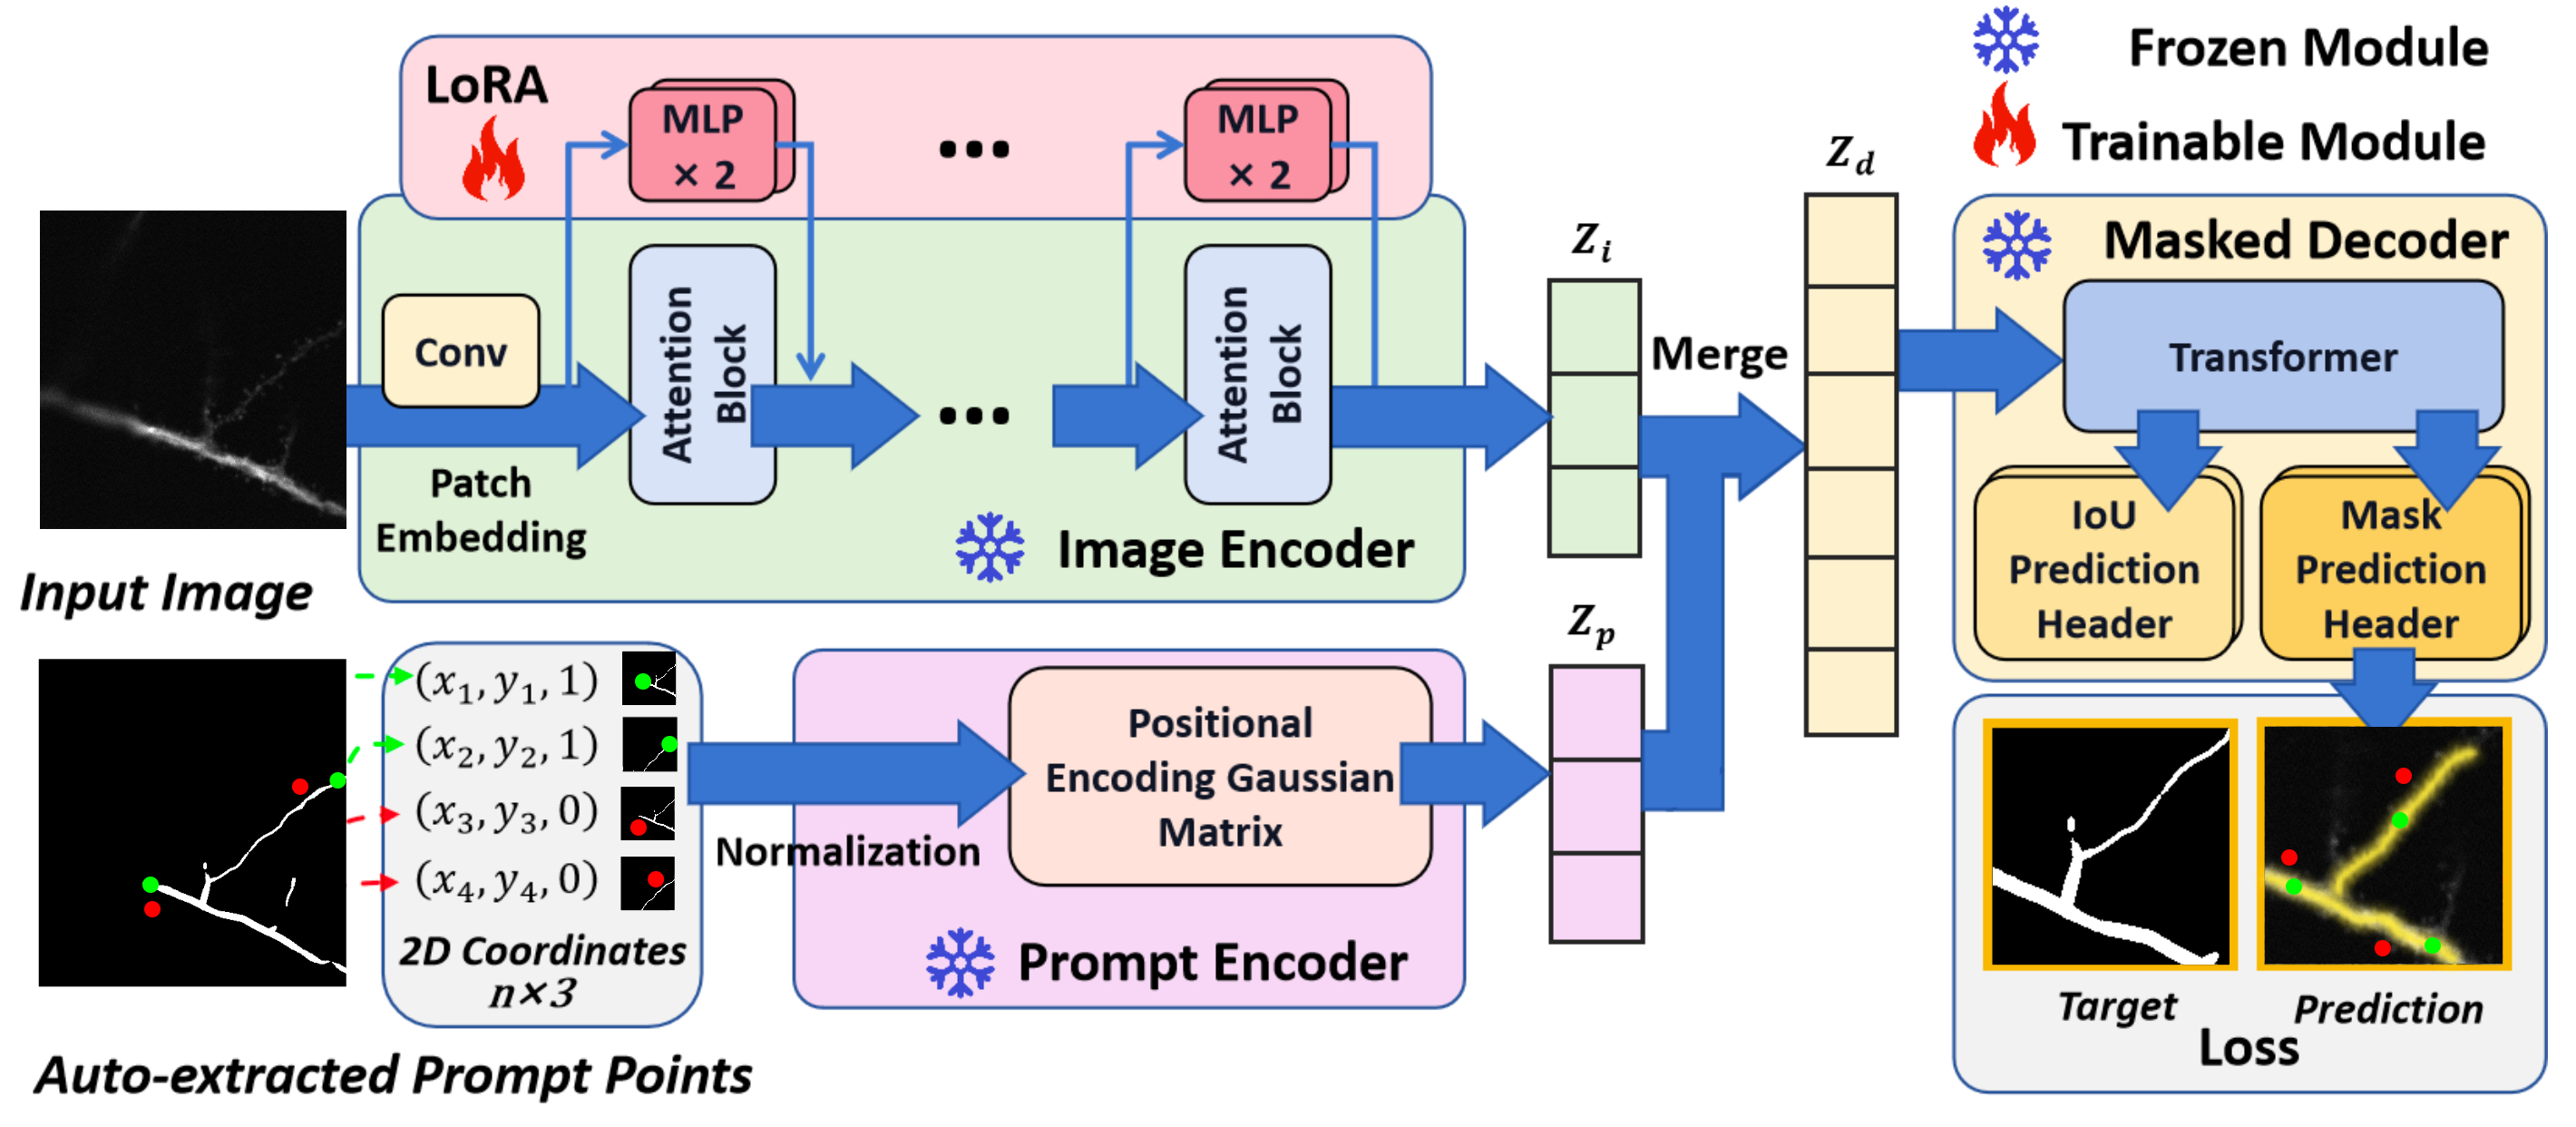
\includegraphics[width=0.95\textwidth]{figures/14_sam_lora_arch.jpg}
\captionof{figure}{Training architecture for \gls{SAM}+\gls{LoRA}. Only the \gls{LoRA} adapters in the image encoder are trainable (marked in red); the prompt encoder and decoder remain frozen. Automatically extracted positive (green) and negative (red) points are encoded and fused with image features to predict the dendrite mask. Image adapted from: \cite{Wang_2023}}
\label{fig:sam_lora_arch}
\end{center}

\subsubsection{\textbf{Fine-tuning Setup}}
For \gls{SAM}+\gls{LoRA}, fine-tuning was implemented by injecting \gls{LoRA} modules into the attention blocks of \gls{SAM}’s image encoder. Each attention block was modified by adding two trainable low-rank matrices ($A \in \mathbb{R}^{d \times r}$ and $B \in \mathbb{R}^{r \times d}$, where $r = 4$ and $d$ is the hidden dimension of the projection), which were inserted into the \gls{MLP} projections. This allowed us to adapt the model to the dendritic segmentation task while keeping the majority of \gls{SAM}’s parameters frozen. The prompt encoder and mask decoder were entirely fixed during training, ensuring that the core behavior of \gls{SAM} remained stable. The only learnable weights were the \gls{LoRA} parameters, resulting in a lightweight training setup with approximately 0.2\% of the full model being updated.

The entire training pipeline was implemented in PyTorch within a custom framework developed. The entry points for training and evaluation were handled through training and testing scripts, while model configuration including \gls{LoRA} rank, learning rate, \gls{GPU} usage, logging behavior, and checkpoint naming was controlled through a config file. This modularity allowed rapid experimentation across different architectural variants. The training was performed on a NVIDIA A100 \gls{GPU} (40 GB memory), using mixed-precision (FP16) acceleration for efficiency.

Training was carried out over 50 epochs with a batch size of 8. The optimizer used was AdamW with a learning rate of $2 \times 10^{-5}$ and weight decay of $10^{-4}$. A cosine annealing scheduler was used to gradually decrease the learning rate over the course of training. Checkpoints were saved every 5 epochs for evaluation. Logs and metrics were stored both locally and optionally through Weights \& Biases for experiment tracking.

Input data consisted of 2D image slices and their corresponding binary dendrite masks, streamed from multi-page \gls{TIFF} stacks. A custom PyTorch \texttt{DatasetLoader} class handled data streaming and augmentation. Each slice was normalized to the range $[0,1]$ using min–max scaling and resized to $1024 \times 1024$ to match the expected model input size. For each image-mask pair, prompt points generated online (positive/negative) were passed to the frozen prompt encoder, and the resulting embeddings were merged with the image features in the transformer encoder–decoder pipeline.

The output segmentation mask was supervised using a composite loss function consisting of binary cross-entropy and soft Dice loss, equally weighted \cite{Galdran_2022}. This combination helped balance pixel-level precision and region-level overlap. Importantly, only the \gls{LoRA} parameters received gradient updates, neither the backbone, nor the prompt encoder, nor the decoder were modified. This ensured that all architectural and performance improvements came strictly from \gls{LoRA} adaptation.

This strict isolation of \gls{LoRA}-based fine-tuning, combined with consistent preprocessing, prompting, and loss across experiments, allows direct comparisons to both the original \gls{SAM} and later variants. The final trained models were stored under structured experiment directories and evaluated using the same benchmark protocol as all other models in this work.

% \subsubsection{\textbf{Data Augmentation}}
% To improve robustness and prevent overfitting, a set of on-the-fly augmentations was applied to each input image–mask pair during training. Augmentations were implemented using the Albumentations library and included both geometric and photometric transformations. Geometric operations involved small-angle random rotations (up to $\pm10^\circ$), random 90° rotations, and horizontal and vertical flips. These transformations simulated the natural orientation variance found in microscopy stacks. Photometric augmentations included brightness/contrast adjustments, Gaussian blur, and additive Gaussian noise, helping the model remain resilient to changes in illumination conditions and imaging noise commonly observed across different acquisition sessions.

% All augmentations were applied synchronously to both the grayscale input image and the corresponding dendrite mask, preserving pixel-wise alignment throughout the pipeline. Since prompt points were extracted from the binary mask, it was critical that augmentations were applied \textit{before} prompt generation to ensure spatial consistency. The augmentation operations were applied stochastically for each training patch, resulting in a diverse and unpredictable sampling of augmented views across training epochs. This augmentation policy was kept consistent across all experiments to ensure that any performance differences could be attributed to the model architecture or training strategy rather than changes in input distribution.

\subsubsection{\textbf{Prompt Generation}}
During training, prompt points were generated on-the-fly from the ground truth dendrite masks. For each connected component in the binary mask, one or more positive points were randomly sampled from within the foreground region. Negative prompts were selected from a morphologically dilated boundary surrounding the structure. This contrastive prompting ensured the model received both inclusion and exclusion signals, helping it learn spatial boundaries even in noisy or low-contrast microscopy contexts. All prompts were encoded as $(x, y)$ coordinates with associated binary labels, and passed to the frozen \gls{SAM} prompt encoder.

At test time, prompts were generated directly from the input image using OpenCV’s \texttt{goodFeaturesToTrack} corner detection algorithm \cite{Shi_1994}. The \autoref{fig:sam_lora_prompt_points} shows that a fixed number of \textit{positive points} were extracted from regions of high spatial contrast, ensuring coverage of salient features. To provide negative supervision, the algorithm also sampled an equal number of low-intensity pixels below the mean of the image, treating them as background cues. This method required no access to ground truth annotations during inference and allowed fully automated segmentation at test time. The prompt points were encoded, fused with image features, and forwarded through the frozen decoder to produce segmentation masks. 

\begin{center}
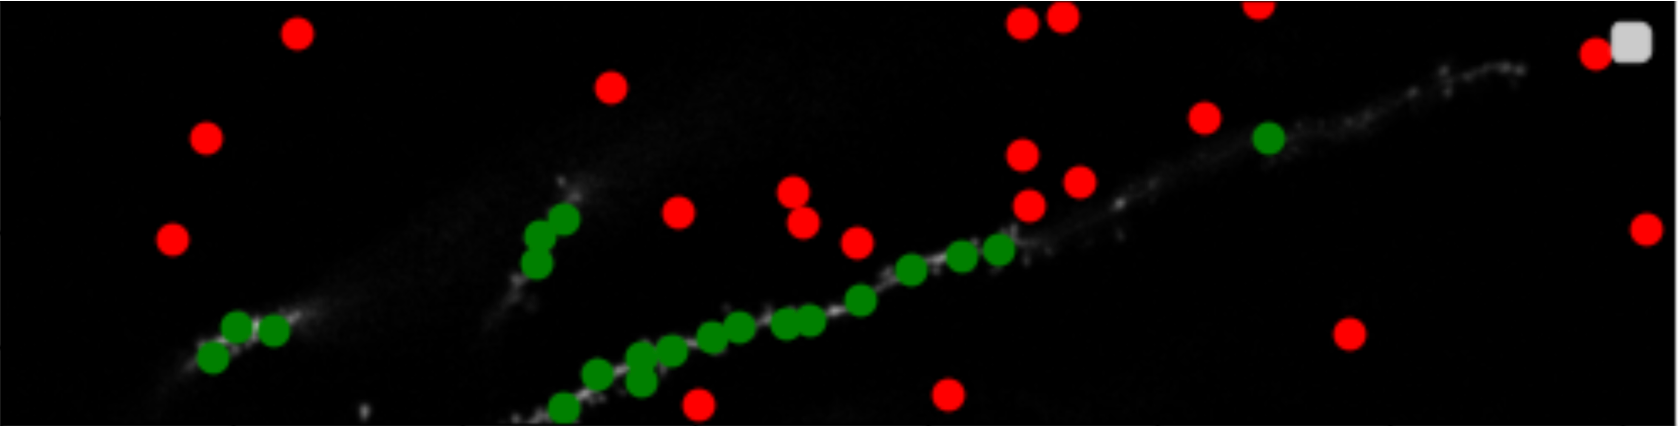
\includegraphics[width=0.95\textwidth]{figures/57_bimap_prompt_points.png}
\captionof{figure}{Prompt Points for \gls{SAM}+\gls{LoRA}. Automatically extracted positive (green) and negative (red) points serves as the prompts for our model. Scale: $0.94\,\mu\text{m}/\text{px}$}
\label{fig:sam_lora_prompt_points}
\end{center}

% \subsubsection{\textbf{Evaluation}}
% \gls{SAM}+\gls{LoRA} was evaluated on the benchmark dataset, entirely separate from the training and validation sets. Each 2D slice was normalized and passed through the model along with prompt points automatically generated from the input image. Positive prompts were extracted using OpenCV’s \texttt{goodFeaturesToTrack} method \cite{Shi_1994}, which identified corners in regions of high local contrast. Negative prompts were sampled randomly from low-intensity background pixels. The model’s outputs were thresholded at 0.5 and saved as binary masks. When ground truth was available, Dice and IoU scores were computed per slice and averaged across the stack. The entire evaluation pipeline was fully automated and logged under timestamped directories for reproducibility

\subsection{Segment Anything Model 2}
All interactive segmentation within the Neuro-\gls{SAM} framework was built upon Segment Anything Model 2, a recent extension of the original \gls{SAM} that introduces temporal and spatial consistency through a memory attention mechanism. While earlier experiments in this work explored standard \gls{SAM} and its low-rank adaptation (\gls{LoRA}) for dendrite segmentation, \gls{SAMv2} was chosen as the backbone model for the final interactive pipeline due to its ability to operate across volumetric data and maintain consistency across slices. Unlike \gls{SAM} and \gls{SAM}+\gls{LoRA}, \gls{SAMv2} was not benchmarked in isolation; instead, it was directly fine-tuned and integrated into our dendrite and spine segmentation modules, which together constitute the core of Neuro-\gls{SAM}.

\subsubsection{\textbf{Architecture}}
While the original \gls{SAM} and its \gls{LoRA}-based adaptation provided strong capabilities, they lacked a mechanism for handling volumetric continuity, something critical for dendritic analysis in 3D microscopy stacks. \gls{SAMv2} addresses this limitation by introducing a memory attention mechanism that allows the model to incorporate contextual information from neighboring slices. This is particularly useful when segmenting dendritic shafts that may span multiple frames but appear intermittently due to signal dropout or imaging noise. In Neuro-\gls{SAM}, this architecture proved instrumental in preserving topological consistency and reducing frame-wise segmentation drift. By integrating both short-range and long-range dependencies across z-slices, \gls{SAMv2} served as the structural backbone for the entire interactive pipeline, supporting both dendrite and spine segmentation in 3D.

\subsubsection{\textbf{Role in Neuro-\gls{SAM}}}
\gls{SAMv2} served as the core segmentation model within the Neuro-\gls{SAM} pipeline. Two instances of the \gls{SAMv2} architecture were separately fine-tuned: one for dendrite segmentation and another for spine segmentation. This modular reuse allowed the model to be tailored to the structural and visual characteristics of each task while maintaining architectural consistency across the pipeline. Both fine-tuned variants leveraged \gls{SAMv2}’s memory-based architecture to improve continuity across volumetric stacks. All training details, data handling procedures, prompt strategies, and post-processing steps involving \gls{SAMv2} are discussed in detail in the Neuro-\gls{SAM} section that follows.

\section{Neuro-SAM}
Building on the insights from previous experiments, Neuro-\gls{SAM} was developed as an interactive segmentation framework tailored specifically for dendritic structures and dendritic spines in volumetric microscopy data. Unlike static segmentation pipelines, Neuro-\gls{SAM} enables users to interactively trace individual dendrites, perform high-fidelity segmentation, detect spines in 3D, and segment them all within a unified interface. The framework is modular by design and leverages two independently fine-tuned instances of \gls{SAMv2}: one specialized for dendrite segmentation and the other for spine segmentation. Combined with a memory-aware architecture, automated prompt generation strategies, and a 3D visualization environment in Napari, Neuro-\gls{SAM} provides precise and adaptable segmentation capabilities that reflect the workflow of real neuroscience annotation tasks.

\subsection{System Overview}
Neuro-\gls{SAM} is designed as a modular, interactive framework for segmenting dendrites and dendritic spines from volumetric microscopy stacks. The system follows a linear yet flexible workflow that mirrors expert annotation practices: beginning with path selection, followed by dendrite segmentation, spine detection, and finally spine segmentation. Each of these steps is organized as a dedicated module within the Napari interface, allowing users to operate on individual dendritic paths with full visual and structural control.

\autoref{fig:neuro_sam} shows the pipeline with a raw 3D stack, where the user interactively traces one or more dendritic paths using an optimized A* algorithm guided by manually placed waypoints. These traced paths are then passed to a fine-tuned \gls{SAMv2} model for targeted dendrite segmentation. After post-processing, the system generates a localized tubular representation along the segmented dendrite to detect spines along its surface. Detected spines, along with any manually added corrections, are used as prompt points for a second fine-tuned \gls{SAMv2} model specialized for spine segmentation. At each step, users can visualize results in both 2D and 3D, iterate on inputs, and export masks for downstream use. The modular nature of the system allows for precise control over each stage of the segmentation process, aligning the model’s output with biological expectations.

\begin{center}
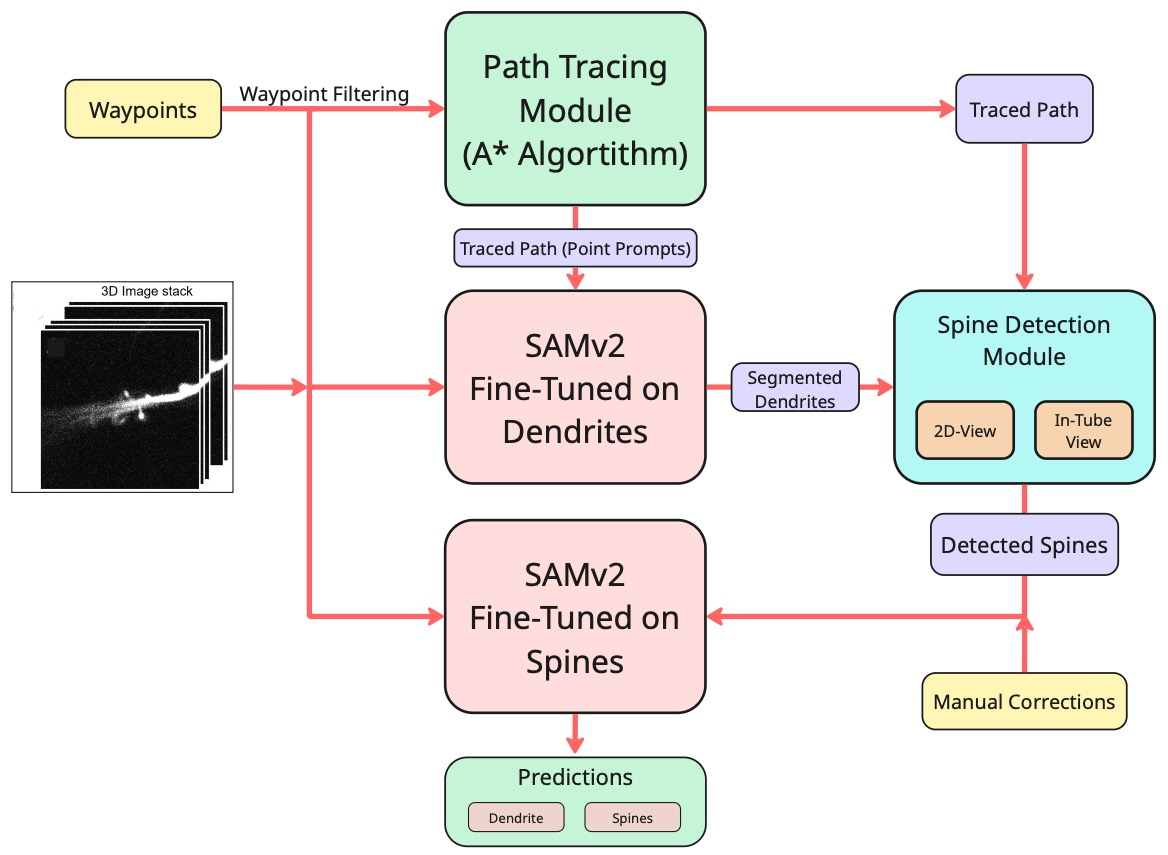
\includegraphics[width=0.95\textwidth]{figures/15_neuro_sam.jpg}
\captionof{figure}{Neuro-\gls{SAM} Pipeline. It takes the 3D stack and the waypoints as an input and produces segmentation masks for dendrites and dendritic spine.}
\label{fig:neuro_sam}
\end{center}

\subsection{Interactive Visualization and User Control}
The user interface of Neuro-\gls{SAM} is implemented entirely within the Napari framework, enabling real-time 2D and 3D visualization of volumetric image stacks alongside interactive annotation and segmentation modules. Upon launching the tool, users are presented with a configurable 3D viewer where raw microscopy stacks can be loaded and visualized as orthogonal slices. To accommodate heterogeneous voxel resolutions across datasets, the interface includes controls for adjusting \textit{X, Y,} and \textit{Z} scaling, ensuring that anisotropic stacks can be rendered and navigated proportionally. These rescaling operations affect both display and downstream processing, and are essential for maintaining spatial accuracy in path tracing and segmentation.

The modular nature of the framework is realized through a multi-tab panel on the right-hand side of the Napari interface. Each tab corresponds to a specific stage in the segmentation workflow including path tracing, dendrite segmentation, spine detection, and spine segmentation. This design enables users to work incrementally, focusing on one dendritic structure at a time without overloading the interface. Within each module, user actions are performed via buttons and mouse-based selections directly on the stack view. The state of the interface including traced paths, intermediate segmentations, and spine prompts is preserved across tabs, allowing users to iteratively refine results without losing context.

Crucially, Neuro-\gls{SAM} is designed around the principle of “guided interactivity”: the system does not require full-volume annotation or batch processing. Instead, it empowers the user to selectively trace and segment individual dendritic branches. This targeted approach reflects real-world annotation workflows in neuroscience, where users typically operate on a per-branch basis due to the complexity and variability of neuronal morphology. Manual inputs such as path waypoints or spine correction clicks are tightly coupled with the model’s prompt-based segmentation mechanism, maintaining a seamless integration between human guidance and model inference. Combined with Napari’s built-in layer management and rendering capabilities, this structure allows for high-resolution inspection, correction, and export of segmented dendrites and spines.

\subsection{Path Tracing Module}
Accurate dendritic segmentation in 3D microscopy data presents unique challenges due to signal dropout, image anisotropy, and faint or discontinuous structures. Direct segmentation of entire volumes often fails to preserve thin, tortuous dendrites, especially when background noise obscures morphology or when branches appear faint in specific slices. To overcome this, Neuro-\gls{SAM} introduces an explicit path tracing step that allows users to interactively define the centerline of dendritic structures before segmentation. This decouples the localization of dendritic trajectories from the segmentation task, enabling precise control over the regions of interest and ensuring that segmentation is performed only along biologically meaningful pathways. By requiring users to click only a few key anchor points, Neuro-\gls{SAM} leverages a guided, structure-aware approach to dendrite identification that proves especially effective in complex or low-contrast regions.

\subsubsection*{\textbf{Brightest Path Tracing Algorithm}}
The original \textbf{brightest-path-lib} \cite{Jha_2023} forms the foundational backbone of our path tracing module. It implements an intensity-aware A* search algorithm specifically designed for tracing neuronal structures in volumetric microscopy images. Unlike traditional A* search that minimizes geometric distance between a source and a target, this approach instead maximizes traversal through bright regions in the image. It takes voxel intensity into consideration and the structures belonging to the dendrites are assigned lower traversal costs.

In this framework, a voxel’s intensity is transformed via a reciprocal cost function, such that brighter voxels are cheaper to traverse. The heuristic component of the A* algorithm remains based on the Euclidean distance, ensuring efficient convergence. The method operates in both 2D and 3D, supporting isotropic and anisotropic data, and includes options for forward-only or bidirectional search to accelerate computation. Importantly, it also allows interactive usage within Napari, wherein users specify start and stop points and immediately visualize the computed trace.

This formulation is particularly powerful for microscopy images where dendritic paths exhibit local intensity maxima but may not always be continuous due to noise, bleaching, or slicing artifacts. The brightness-based cost function compensates for such irregularities by probabilistically favoring plausible structural continuations, even when they temporarily dip in contrast.

\subsubsection{\textbf{Improvements and Optimizations}}
While the original Brightest Path algorithm provides a robust and user-friendly tool, it has several notable limitations when applied to dendrite tracing in high-resolution, anisotropic datasets. Specifically:

\begin{itemize}

     \item{\textbf{Lack of waypoint support}: The algorithm expects a start and end point, with no native support for intermediate guidance points (waypoints), which is limiting when tracing highly twisted dendrites.}


    \item{\textbf{Uniform Z assumption}: The Z points are uniformly distributed across the start and end z range irrespective of checking neighboring z frames for their occurrence.}
    
    \item{\textbf{Limited speed on large volumes}: The original implementation performs a full A* search between points, which becomes computationally expensive as volume size and complexity grow.}
    
    \item{\textbf{No parallelization}: Each path is traced sequentially, limiting real-time usage in interactive environments.}
    
    \item{\textbf{No voxel spacing awareness}: Anisotropic voxel dimensions are not considered during smoothing or cost calculations, which can distort the reconstructed path.}

\end{itemize}

To address these issues, our version introduces several targeted optimizations and design improvements aimed at improving usability, accuracy, and runtime performance:

\begin{itemize}
    

\item{\textbf{Waypoint-Driven Tracing}: Instead of a single path between two points, we allow users to click multiple waypoints. The algorithm automatically identifies the furthest-apart points as start and end, and uses the rest as intermediate guidance.}

\item{\textbf{Z-Aware Waypoint Optimization}: For each 2D waypoint, we perform a local search across Z to find the optimal intensity-consistent Z-layer. This utilizes intensity transition detection (appearance/disappearance) and distributes waypoints intelligently across the dendrite’s 3D span.}

\item{\textbf{Anisotropic B-Spline Smoothing}: After tracing, paths are smoothed using B-spline interpolation that accounts for voxel spacing in X, Y, and Z. This ensures that spatial relationships remain physically meaningful despite voxel anisotropy.}

\item{\textbf{Numba Acceleration}: All performance-critical components including distance calculations, Z-search, and filtering are compiled using Numba \cite{Lam_2015}, reducing runtime significantly without sacrificing accuracy.}

\item{\textbf{Parallelized Segment Tracing}: The overall path is broken into segments between consecutive waypoints, and A* is executed independently on each segment. This enables efficient multi-threaded execution using Python’s ThreadPoolExecuter.}

\item{\textbf{Hierarchical Search with Refinement}: For very large volumes, the algorithm falls back to a coarse A* search on a downsampled image followed by full-resolution refinement in a narrow corridor, ensuring scalability.}

\item{\textbf{Automatic Filtering of Redundant Waypoints}: Waypoints closer than a certain Euclidean threshold are filtered out, reducing noise and improving both path fidelity and performance.}
\end{itemize}

Collectively, these improvements transform the original concept into a highly flexible, anisotropy-aware, and interactive path tracing module suitable for efficient dendrite analysis in neuroscience imaging. They also serve as a foundational step before segmentation, ensuring that the downstream segmentation operates on biologically accurate dendritic traces.

\subsubsection{\textbf{Waypoint-Aware Brightest Path Tracing (Pseudocode)}}

The following algorithm  \ref{alg:enhanced_path_tracing} outlines the core logic of our improved waypoint-driven, anisotropy-aware path tracing algorithm. This modular architecture enables flexible user interaction, intelligent Z-aware optimization, parallel execution, and hierarchical fallback for large datasets.

\begin{algorithm}[htb]
\footnotesize
\begin{algorithmic}[1]
    \State \textbf{Input:} 3D image volume $I$, list of user-clicked points $P$ (in $[z, y, x]$), voxel spacing $s_x$, $s_y$, $s_z$
    \State \textbf{Output:} Brightest path $\pi$ connecting the points in $P$
    \State 
    \State \textbf{Step 1: Preprocessing}
    \State Convert list $P$ to numpy array and extract start, end, and intermediate waypoints
    \State If Z-range optimization is enabled:
    \State \hspace{1em} Use intensity transition analysis to adjust Z-values of start and end
    \State \hspace{1em} Apply intensity-aware Z-optimization to distribute waypoints
    \State Apply minimum-distance filtering to remove close waypoint duplicates
    \State 
    \State \textbf{Step 2: Segment-wise Brightest Path Search}
    \For{each segment between consecutive points $(p_i, p_{i+1})$ in path}
        \State Compute 3D nanometer distance using voxel spacing
        \State Determine search strategy:
        \State \hspace{1em} Use full-resolution or hierarchical A* search based on segment length and image size
        \If{strategy is hierarchical}
            \State Downsample image conservatively using max pooling
            \State Perform coarse A* search in downsampled image
            \State Refine path at full resolution in a narrow corridor
        \Else
            \State Perform bidirectional A* search between $p_i$ and $p_{i+1}$
        \EndIf
        \State Append resulting segment path to output $\pi$
    \EndFor
    \State 
    \State \textbf{Step 3: Post-processing}
    \If{smoothing is enabled}
        \State Apply anisotropic B-spline smoothing with voxel spacing $s_x$, $s_y$, $s_z$
        \State Preserve start and end point coordinates
    \EndIf
    \State 
    \State \Return Full path $\pi$ as ordered array of $[z, y, x]$ coordinates
\end{algorithmic}
\caption{Waypoint-Aware Brightest Path Tracing}
\label{alg:enhanced_path_tracing}
\end{algorithm}

The proposed path tracing module forms a fundamental building block of Neuro-\gls{SAM}, enabling accurate and user-guided dendritic path extraction across volumetric microscopy data. By coupling intensity-aware bidirectional A* search with Z-optimization, waypoint refinement, and anisotropic B-spline smoothing, our system delivers both speed and precision. Crucially, it empowers researchers to interactively define complex dendritic routes in noisy or anisotropic environments, a task traditional methods struggle with.

Having traced the structural backbone, the next step lies in understanding how this path integrates with downstream components of Neuro-\gls{SAM}, especially in facilitating targeted segmentation and spine detection. We now turn our attention to the dendrite segmentation module.

\subsection{Dendrite Segmentation Module}
To perform localized dendrite segmentation in Neuro-\gls{SAM}, we fine-tuned a dedicated instance of \texttt{\gls{SAMv2}} specifically for this task. This model was not used in its original form but instead underwent targeted domain adaptation using custom prompt strategies, a volumetric patch-based inference setup, and structured loss supervision on our dataset. Unlike global segmentation pipelines, our approach required high-fidelity masks aligned with manually traced dendritic paths. This necessitated both architectural compatibility with localized inference and the flexibility to train with overlapping patches and sparse supervision. Every component of the training and inference stack from dataloading to optimization was purpose-built to support high-precision segmentation in noisy, anisotropic microscopy volumes. 

% \subsubsection{\textbf{Dataloader}}
% For training, a custom streaming dataloader (\texttt{DataGeneratorStream}) was implemented on top of the \gls{DeepD3} dataset. The loader dynamically sampled 2D slices from randomly chosen 3D image stacks and rescaled them to a fixed target resolution of 94 nm/pixel. To ensure informative samples, only slices containing at least 100 dendrite foreground pixels were retained. Prompt points were generated on-the-fly using a foreground–background contrast strategy that sampled connected components within dendrite masks and their neighboring regions. Preprocessing and data augmentation were applied in the same manner as described earlier, ensuring consistency across all models.

\subsubsection{\textbf{Fine-tuning Setup}}
The fine-tuning process was conducted on the \texttt{\gls{SAMv2}} architecture, with a systematic evaluation of multiple model variants and image resolutions. Specifically, we experimented with the \texttt{tiny}, \texttt{small}, and \texttt{base-plus} backbones, each trained at different input resolutions: 128, 256, 512, and 1024 pixels. These experiments were performed to understand the trade-offs between segmentation accuracy, memory consumption, and inference speed. We ultimately selected \texttt{SAMv2-small} with an input resolution of 128$\times$128 for integration into Neuro-\gls{SAM}, as it provided a robust balance between performance and computational efficiency on high-throughput microscopy datasets. A custom dataloader was implemented ensuring smooth sampling and data augmentation of 2D slices from the 3D stacks. 

Fine-tuning was performed end-to-end, with all core components \texttt{image encoder}, \texttt{prompt encoder}, and \texttt{mask decoder} set to trainable mode. Optimization was carried out using \texttt{AdamW} \cite{Loshchilov_2019} with a learning rate of $1 \times 10^{-5}$ and a weight decay of $4 \times 10^{-5}$, chosen to ensure stable convergence in a low-data, high-noise regime. Training leveraged mixed-precision arithmetic using PyTorch's \texttt{torch.amp} with automatic casting and gradient scaling via \texttt{GradScaler}.

The input pipeline generated prompts during training using the \texttt{PromptGeneration} module. These prompts were encoded using the \gls{SAMv2} prompt encoder and fused with high-resolution image features within the hierarchical decoder to produce a set of segmentation masks and associated confidence scores.
The training objective was a combination of two loss components. The primary loss was a binary cross-entropy between the predicted mask logits (after sigmoid activation \cite{Zhai_2023}) and the corresponding dendrite mask. An auxiliary score prediction loss penalized the absolute difference between the model's confidence score and the true \gls{IoU} \cite{Cheng_2021}, scaled by a factor of 0.05. This dual-loss formulation helped improve both the structural accuracy of the segmentation and the reliability of the model’s internal confidence estimation.

Training ran for 100,000 steps with a batch size of 32 and the training performance was continuously monitored via Weights \& Biases \cite{WandB}. Every 500 steps, a full validation cycle was performed on the validation dataset, measuring Dice coefficient \cite{Shamir_2019}, \gls{IoU}, and overall loss. Augmentations were disabled during the validation to ensure consistency across epochs. All training and validation logs were automatically recorded and checkpoints were saved. Although we ran the full training cycle, the model started to converge after 8,000 iterations which is shown in \ref{sec:sam2_plots}. 

\subsubsection{\textbf{Prompt Strategy for Dendrites}}
Dendritic structures in 3D microscopy data present a unique challenge for segmentation due to their elongated geometry, variable brightness, and sparse annotations. In Neuro-\gls{SAM}, careful attention was given to designing distinct yet coherent prompt strategies for both training-time supervision and inference-time prediction, ensuring robust generalization and precise alignment with traced dendritic paths.


\paragraph{Training-Time Prompt Generation}

To train the \texttt{\gls{SAMv2}} model effectively on dendritic masks, we implemented a custom prompt generation strategy implemented via the \texttt{PromptGeneration} class. This module dynamically generated spatial prompts comprising both positive and negative points for every training sample during each iteration. Positive points were sampled from connected foreground components in the dendrite mask, where each component (filtered by a minimum area threshold) contributed at most one prompt. This ensured spatial diversity while avoiding redundancy. The number of positive and negative prompts was parameterized through command-line flags (\texttt{----ppn}, \texttt{----pnn}), enabling systematic exploration of prompt density.

Negative prompts required more careful construction. Rather than random background sampling, we adopted a boundary-aware strategy that first dilated each dendritic component by two radii: an inner and an outer boundary band (typically 3–9 and 3–20 pixels, respectively). Negative prompts were then sampled exclusively from within the ring formed by subtracting the inner dilation from the outer one. This approach encouraged the model to learn precise object boundaries, particularly in cluttered cellular environments. Additionally, a fallback mechanism ensured sampling stability by randomly drawing from background pixels if not enough structured negatives could be found. All sampling operations were seeded for reproducibility. \autoref{fig:training_prompts} shows an example of the training prompts generation, blue being the positve (foreground) points while red being the negative (background) points. 

\begin{center}
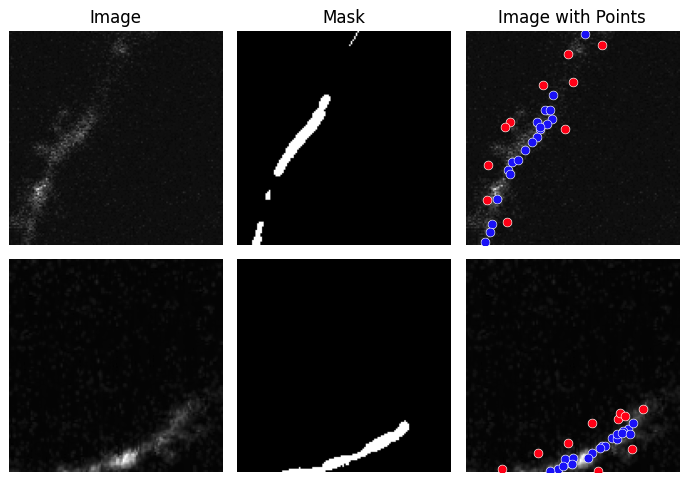
\includegraphics[width=0.9\textwidth]{figures/16_training_prompts.png}
\captionof{figure}{Prompt Points generated on the fly during training. The blue points show the positive (foreground) points and red points are the negative (background) points. Scale: $0.94\,\mu\text{m}/\text{px}$}
\label{fig:training_prompts}
\end{center}

\paragraph{Inference-Time Prompt Construction}

During inference in the Neuro-\gls{SAM} pipeline, the prompt strategy was fundamentally different: prompts were no longer randomly sampled, but rather derived directly from the manually traced dendritic path and its local context. The path, constructed interactively by the user, provided a spatial prior for where dendrites are expected to lie. For each 2D slice being segmented, the traced path was intersected with the corresponding image plane to extract candidate foreground (positive) points. These were projected into patch-local coordinates and, if needed, subsampled to ensure coverage while maintaining efficiency.

To complement these foreground prompts, background (negative) prompts were generated using a convex-hull-based envelope around the path. The algorithm constructed a narrow shell surrounding the positive region, defining an inner and outer boundary based on fixed radial distances. Negative points were then sampled from within this band, avoiding overlap with the dendrite core. This technique mimicked the negative prompt strategy used during training while adapting it to the path geometry produced by the user. If the convex hull could not be constructed (e.g., due to sparse waypoints), a fallback random sampling strategy was used instead. \autoref{fig:testing_prompts} shows the role of testing prompts. Positive prompts in the center of the dendrite (derived from the traced path) and a boundary region from where we sampled the negative prompts. It also shows how well the prompt points guide the model prediction on a patch from the benchmark dataset.

\begin{center}
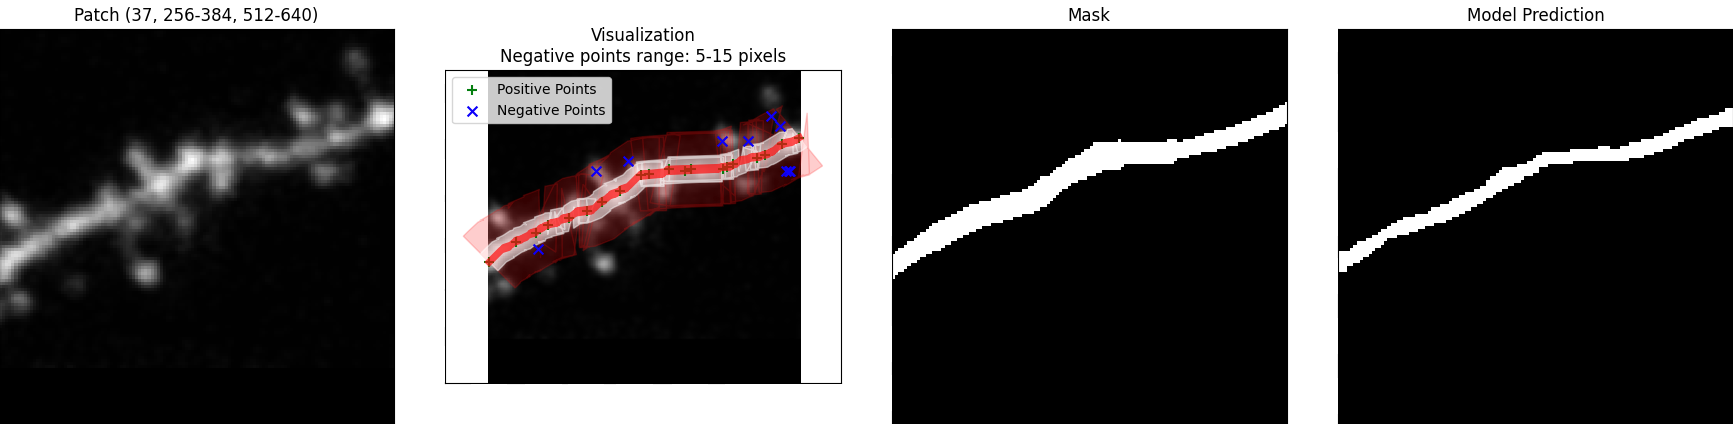
\includegraphics[width=1.0\textwidth]{figures/17_testing_prompts.png}
\captionof{figure}{Inference Prompt points along with model prediction. The first image shows the image patch, second shows the red region as foreground with a boundary region with negative points. The image third and fourth shows the ground truth and predicted mask. Scale: $0.94\,\mu\text{m}/\text{px}$}
\label{fig:testing_prompts}
\end{center}

Importantly, the prompts were not limited to a single slice. To improve robustness, particularly in anisotropic volumes, Neuro-\gls{SAM} allowed prompts to be collected from a small temporal window, typically $\pm 4$ slices around the current frame; thereby injecting limited 3D context into each segmentation operation without requiring full volumetric inference. This was particularly useful for guiding segmentation in frames with poor contrast or missing features.

In both training and inference, our prompt design emphasized \textit{locality}, \textit{structure-awareness}, and \textit{noise tolerance}, enabling \texttt{\gls{SAMv2}} to produce accurate segmentations that conform tightly to biological reality.

% \subsubsection{\textbf{Evaluation}}

% The fine-tuned \texttt{SAMv2} model for dendrite segmentation was evaluated on a dedicated validation split from our dataset, with benchmark stacks strictly excluded to preserve an unbiased test set for later pipeline-level assessment. Validation was performed every 500 training iterations and consisted of 20 randomly sampled batches, each processed without any form of augmentation to ensure metric consistency across epochs. The batch size for validation matched the training configuration to maintain comparable memory usage and computational load.

% Performance was quantified using a combination of pixel-level and object-level metrics. The primary segmentation accuracy measure was the Dice coefficient \cite{Shamir_2019}, chosen for its sensitivity to both precision and recall in binary mask prediction and its suitability for elongated structures such as dendrites. The Intersection-over-Union (IoU) \cite{Cheng_2021} was computed alongside Dice to provide a complementary perspective on mask overlap quality, particularly valuable for cases with small absolute foreground area. The total validation loss was also recorded, incorporating both the binary cross-entropy segmentation loss and the auxiliary score regression loss, enabling the tracking of not only spatial accuracy but also confidence calibration.

% For each validation batch, the predicted masks were binarized at a fixed threshold of 0.5 after sigmoid activation. The IoU was computed as:


% \[
% IoU = \frac{|P \cap G|}{|P \cup G|}
% \]

% where $P$ and $G$ denote the sets of predicted and ground truth foreground pixels, respectively. Meanwhile the Dice Score can be computed as:

% \[
% Dice = \frac{2 |P \cap G|}{|P| + |G|}
% \]

% These metrics were averaged at the end of 20 batches to yield mean validation scores for each evaluation step. In addition to numerical metrics, qualitative inspection was carried out by overlaying predicted masks on raw validation images, allowing rapid identification of common failure modes such as dendrite discontinuities or over-extension into background structures.

% The evaluation process played a critical role in model selection. Among the multiple variants trained during experimentation, the \texttt{SAMv2-small} model with 128$\times$128 input resolution was selected for integration into the Neuro-\gls{SAM} pipeline, as it consistently achieved a strong balance of high Dice/IoU scores, low validation loss, and rapid inference suitable for interactive annotation workflows.

\subsubsection{\textbf{Integration with Neuro-\gls{SAM} Pipeline}}

The fine-tuned \texttt{\gls{SAMv2}-small} model was fully embedded into the Neuro-\gls{SAM} interactive environment to enable seamless, localized dendrite segmentation directly within the existing dendrite tracing workflow. Once a user traces a dendritic path using the \textbf{Path Tracing Module}, the 3D coordinates of this path are used to define a spatially bounded \gls{ROI} within the anisotropic volume. This \gls{ROI} selection step is crucial, as it ensures that the segmentation model operates only on relevant sub-volumes, reducing inference time and minimizing false positives in unrelated regions.

Within this \gls{ROI}, the segmentation process follows the volumetric, overlapping patch-based inference strategy described earlier. The module divides each relevant frame into $128 \times 128$ pixel patches with a 50\% stride overlap, ensuring complete coverage of dendritic structures and robust handling of edge effects. Each patch is processed independently by the fine-tuned \texttt{\gls{SAMv2}} model using prompt points derived from the traced path, enabling localized predictions that align with the specific dendritic branch being segmented. The resulting patch-level masks are then merged via adaptive averaging, where pixel-level confidence thresholds are dynamically adjusted based on patch overlap counts to preserve structural continuity.

After merging, the raw binary masks undergo dendrite-specific post-processing. This includes hole filling to preserve the solid tubular morphology, morphological closing in both horizontal and vertical orientations to connect discontinuities, and removal of small isolated regions below a user-defined size threshold. Additionally, a path-proximity validation step discards any mask regions that deviate beyond a set spatial distance from the traced dendrite, effectively eliminating noise while retaining fine peripheral branches.

The segmented mask is immediately overlaid on the original 3D stack within the Napari-based Neuro-\gls{SAM} viewer, using a high-contrast color assigned to distinguish it from other dendrites and spines in the session. Users can interactively refine results by adjusting post-processing parameters, retracing path segments, or re-running segmentation with alternative patch sizes or prompt configurations. The final, validated masks can be exported as multi-frame TIFFs for downstream analysis or directly passed to subsequent modules in the pipeline.

By integrating the segmentation model in this tightly coupled manner, Neuro-\gls{SAM} ensures that dendrite segmentation is not a standalone step, but rather a fully interactive, path-aware process that naturally transitions into the spine detection module, where the segmented dendritic shafts form the structural basis for localized spine candidate generation.

\subsection{Spine Detection Module}

Detecting dendritic spines is an inherently challenging task due to their small size, morphological variability, and inconsistent contrast within noisy 3D microscopy volumes. To address this, the spine detection module in Neuro-\gls{SAM} employs a geometry-aware, intensity-guided pipeline that tightly couples with the previously traced dendritic paths. Rather than relying on conventional 3D blob detection or global segmentation strategies, this module performs localized dual-view analysis at discrete positions along the dendritic shaft. It extracts focused 2D views and orthogonal cross-sections collectively referred to as \textit{tube data} around each point along the traced path, enabling the system to identify spines with greater spatial and directional accuracy. Confirmed candidates are then refined through intensity consistency checks and spatial grouping, producing robust 3D coordinates for downstream segmentation. The resulting detections serve as direct input to the spine segmentation pipeline within Neuro-\gls{SAM}.

\subsubsection{\textbf{Tube Data Generation}}

To enable localized spine detection along the dendritic shaft, we construct a series of context-rich frames, termed \textit{tube data}, at equidistant points along the traced dendrite path. Each frame encodes local spatial information in both the axial (XY) and orthogonal cross-sectional directions referred to as \textit{tube data}. Given a discrete path \(\{\mathbf{p}_0, \mathbf{p}_1, \ldots, \mathbf{p}_{N-1}\}\) in 3D space, we compute tangent vectors via central differencing and derive a pair of orthonormal basis vectors \((\mathbf{up}_i, \mathbf{right}_i)\) at each location, defining a plane perpendicular to the local dendritic trajectory.

At every position \(\mathbf{p}_i\), three views are extracted:

\begin{itemize}
  \item A \textbf{zoomed patch} in the XY plane, centered at \(\mathbf{p}_i\), capturing local frontal features for 2D blob detection.
  \item A \textbf{tubular plane}, generated orthogonally to the dendrite axis using the basis vectors \(\mathbf{up}_i\) and \(\mathbf{right}_i\), for detecting off-axis structures.
  \item An optional \textbf{reference mask}, we got from the dendrite segmentations.
\end{itemize}

\begin{center}
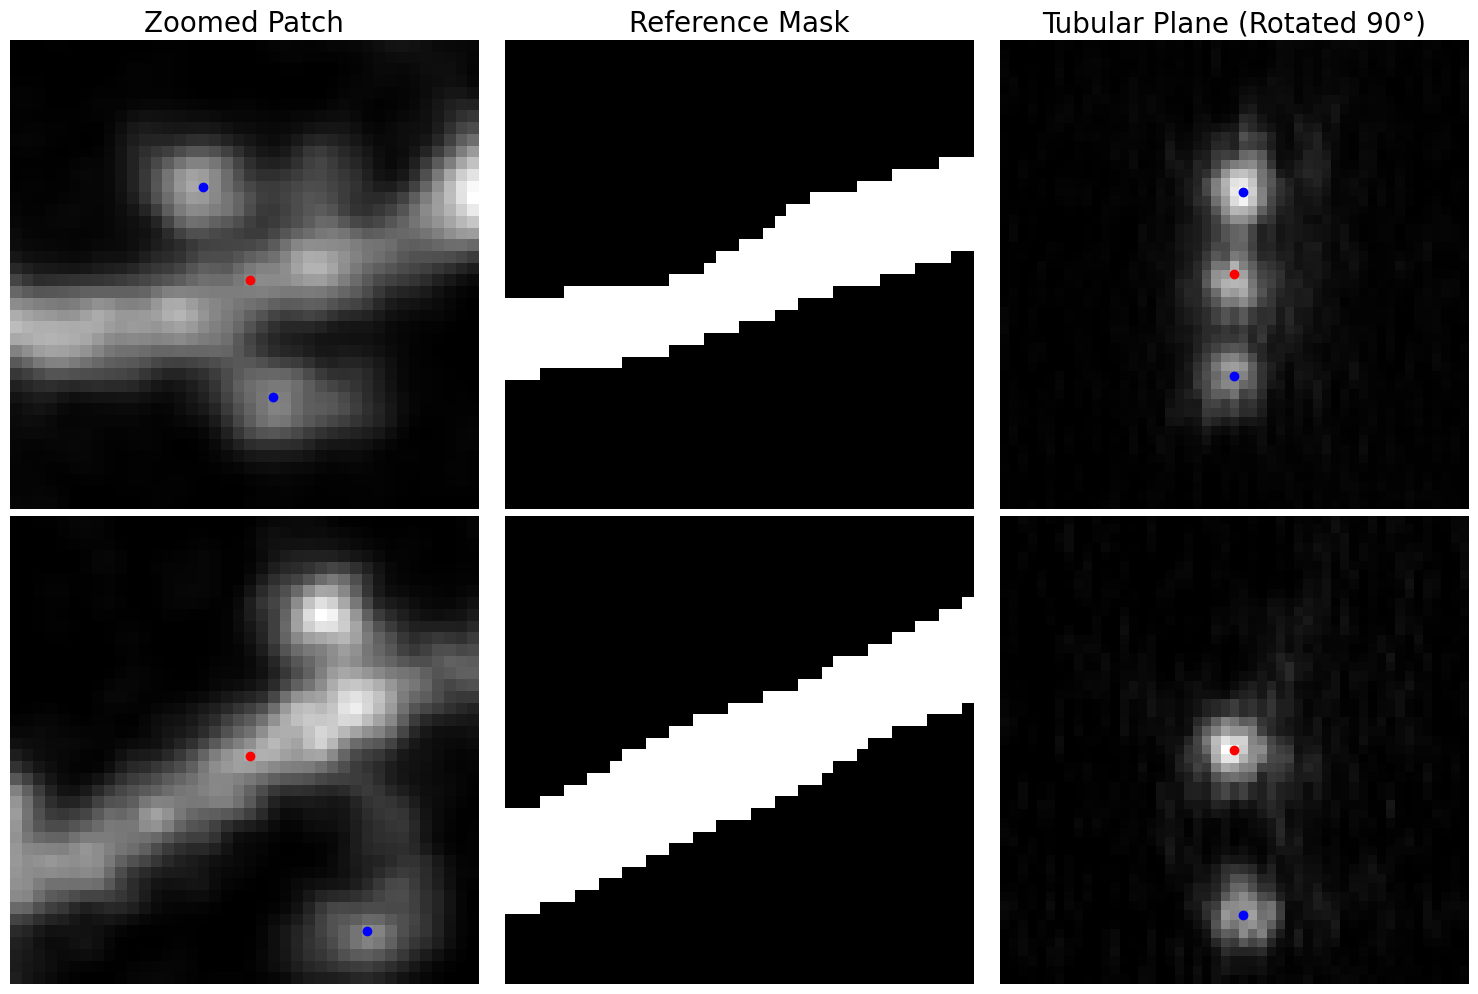
\includegraphics[width=0.8\textwidth]{figures/19_tube_data.png}
\captionof{figure}{The plot shows a 2D zoomed view of the dendrite, a reference mask and an in-tube view of the dendrite. The red point displays the center of the dendrite (obtained from path tracing), and the blue point displays the spines that are projecting outwards in the \gls{FOV}. Scale: $0.94\,\mu\text{m}/\text{px}$}
\label{fig:tube_data}
\end{center}

To compute the tubular plane, we define a 2D grid of size \((2w + 1) \times (2w + 1)\) centered on \(\mathbf{p}_i\), where \(w\) denotes the half-width in pixels. Each grid cell is mapped to a corresponding 3D coordinate in the original volume via:

\[
\mathbf{q}_{i,j,k} = \mathbf{p}_i + (j - w) \cdot \mathbf{up}_i + (k - w) \cdot \mathbf{right}_i,
\quad \text{where } j, k \in \{0, \ldots, 2w\}.
\]



These coordinates are rounded to the nearest voxel and sampled if within bounds. The resulting plane yields a cross-sectional slice orthogonal to the dendrite, faithfully aligned with its local direction of propagation.

This process is implemented using efficient, Numba-parallelized routines and supports reference blending for enhanced visualization. The full set of extracted frames constitutes the input to subsequent dual-view spine detection and geometric consistency filtering, detailed next.

\subsubsection{\textbf{Dual-View Spine Detection}}
Building on the localized \textit{tube data}, we now perform dual-view blob detection to identify dendritic spines. Global approaches often misinterpret fine structures near the shaft, so our method relies on spatially constrained, multi-view analysis for precise detection.

Each tube frame provides two complementary views to detect potential spine candidates. The first is the frontal 2D patch, a square XY slice centered on the dendritic path point. On this patch, we apply a \gls{LoG} \cite{Kong_2013} filter to highlight blob-like intensity structures. To avoid misidentifying the dendritic shaft itself, we subtract a reference mask before detection, effectively suppressing the central dendritic region. In parallel, we apply a similar \gls{LoG}-based detection on the \textit{tubular view}. This orthogonal detection step captures spines that may not be prominent in the frontal XY plane due to orientation or noise. The outputs of this step are candidate blob coordinates identified in the tubular view, relative to the orientation of the dendrite at each point.

To consolidate detections from both views, we perform pairwise matching between 2D frontal blobs and tubular blobs based on geometric consistency. For each frontal candidate, we compute its direction vector relative to the center of the patch and compare it with the local dendrite orientation at that frame. Similarly, each tubular blob is represented by a vector from the center of the tubular plane. These vectors are converted to angles, and angular consistency is computed via dot product and cross product formulations. Only pairs with angular differences below a defined threshold (typically \(20^\circ\text{–}25^\circ\) are considered.

The Euclidean distance of each blob from the patch center is compared across both views. The matching score for a pair is computed as a weighted combination of angular difference and distance mismatch, controlled by an angle-weighting hyperparameter (e.g., 0.7). The best-matching tubular blob for each 2D frontal blob is selected, and only those with scores below a strict threshold are retained as confirmed candidates. This cross-view verification ensures that final spine detections are not only morphologically plausible, but also directionally consistent with the underlying dendritic shaft.

Following the initial detection, spine candidates are grouped based on spatial proximity in the lateral plane to merge redundant detections across adjacent frames. Within each group, the most structurally distinct instance, typically the brightest or most contrasted is selected. This spine is then re-evaluated across neighboring slices to assess its visibility using localized intensity analysis. Only those candidates consistently distinguishable from the background are retained. The final set of tracked spines is both spatially unique and temporally validated, ensuring reliable input for the downstream segmentation module.

While the automated detection pipeline captures the majority of spine candidates, Neuro-\gls{SAM} also allows users to manually annotate spines via interactive point placement within the 3D interface. These manual inputs are treated identically to algorithmic detections, integrated into the tracking and refinement workflow without distinction. This ensures flexibility in handling edge cases or atypical morphologies that escape automated detection. With a finalized set of spatially verified spine coordinates, we next shift focus to the segmentation of these structures, where localized prompts are leveraged to extract fine-grained spine masks.

\subsubsection{\textbf{Spine Detection Algoritm (Pseudocode)}}

The entire spine detection workflow is summarized in Algorithm \ref{alg:spine_detection}, which outlines the key steps from dual-view blob extraction and angle-based matching to manual integration and final tracking with intensity-aware validation. This procedure ensures spatially consistent and morphologically relevant spine candidates, ready for downstream segmentation.

\begin{algorithm}[htb]
\footnotesize
\begin{algorithmic}[1]
    \State \textbf{Input:} 3D image volume $\mathcal{I}$, traced dendrite path $\mathcal{P}$, segmentation mask $\mathcal{M}$, optional manual points $\mathcal{U}$
    \State \textbf{Output:} 3D spine coordinates $\mathcal{S}$

    \State 
    \State \textbf{Step 1: Tube Data Construction}
    \For{each path point $\mathbf{p}_i \in \mathcal{P}$}
        \State Compute tangent vector using central difference
        \State Generate local orthonormal basis $(\mathbf{up}_i, \mathbf{right}_i)$
        \State Sample:
        \State \hspace{1em} (a) Frontal XY patch centered at $\mathbf{p}_i$
        \State \hspace{1em} (b) Orthogonal tubular plane via coordinate projection
        \State \hspace{1em} (c) Reference patch from $\mathcal{M}$ (optional)
        \State Store all three views in frame data $\mathcal{T}[i]$
    \EndFor

    \State 
    \State \textbf{Step 2: Spine Blob Detection}
    \For{each frame $t \in \mathcal{T}$}
        \State Apply LoG blob detection on frontal patch
        \State Apply LoG blob detection on tubular plane 
        \State Extract blob coordinates in both views
    \EndFor

    \State 
    \State \textbf{Step 3: Angle-Based Matching Across Views}
    \For{each frontal blob in frame $t$}
        \For{each tubular blob in the same frame}
            \State Compute relative angle with dendrite tangent
            \State Compute radial distance from view center
            \State If both angle and distance criteria are satisfied:
            \State \hspace{1em} Add to list of matched spine candidates
        \EndFor
    \EndFor

    \State 
    \State \textbf{Step 4: Manual Point Integration}
    \If{manual spine points $\mathcal{U}$ are provided}
        \State Merge $\mathcal{U}$ with matched spine candidates
    \EndIf

    \State 
    \State \textbf{Step 5: Spine Tracking}
    \State Group nearby spines across frames to avoid duplicates
    \For{each spine group}
        \State Select representative spine based on intensity
        \State Track visibility across neighboring Z-slices
        \If{visible in any frame}
            \State Add frame-local positions to final spine list $\mathcal{S}$
        \EndIf
    \EndFor

    \State 
    \State \Return Final spine coordinates $\mathcal{S}$
\end{algorithmic}
\caption{Spine Detection using Dual-View Matching and Intensity-Aware Tracking}
\label{alg:spine_detection}
\end{algorithm}

\subsection{Spine Segmentation Module}
While dendrite segmentation provides the structural backbone for Neuro-\gls{SAM}, accurate segmentation of individual dendritic spines requires a separate, specialized treatment. These micron-scale protrusions exhibit high shape variability, low contrast, and often cluster near dense dendritic regions posing a substantial challenge for segmentation algorithms. To address this, we fine-tuned a dedicated instance of \texttt{SAMv2} specifically for spine segmentation using candidate-aware prompts and overlapping patch-based inference. Unlike dendrites, spine masks tend to be sparse, disconnected, and morphologically heterogeneous, demanding both precise center localization and shape-aware post-processing. Our model operates on localized \gls{ROI}s defined by the previously detected spine candidates, optionally enriched with manual point corrections, and leverages the model's internal morphological priors to produce clean, circular spine masks suitable for downstream analysis and quantification.

% \subsubsection{\textbf{Dataloader}}
% For training the spine segmentation model, we developed a custom streaming dataloader, \texttt{SpineGeneratorStream}. This dataloader dynamically samples 2D patches from randomly selected 3D volumes and resizes each patch to 128$\times$128 pixels while preserving a fixed spatial resolution of 94~nm/pixel using voxel metadata. Only samples with at least 100 pixels of annotated dendritic or spine content were retained, ensuring that the model was consistently exposed to informative training regions.

% Each training sample comprises three aligned channels: the raw image patch, a binary dendrite mask, and a corresponding binary spine mask. These masks are used not only for supervision but also for generating training prompts on-the-fly. Data augmentation is performed in real-time using a composite of geometric (rotations, flips), photometric (brightness, contrast), and noise-based transformations via \texttt{Albumentations}. This dynamic pipeline enables highly diverse training while avoiding redundant disk-based patch storage.

% To facilitate point-based segmentation learning, the dataloader invokes a lightweight \texttt{PromptGeneration} module that identifies candidate spine centers. It uses distance-transform and watershed segmentation to identify spine center and separate connected spines. These detected centers are converted into positive prompts, while optional background points are sampled from non-spine regions to guide the model in suppressing false positives. This prompt generation is both patch-local and density-aware, enabling flexible supervision even in crowded spine environments.

\subsubsection{\textbf{Fine-Tuning Setup}}

The spine segmentation model was fine-tuned on the \texttt{\gls{SAMv2}} architecture, targeting localized instance segmentation of dendritic spines using patch-wise point prompts. Unlike the dendrite segmentation pipeline, which required broader path-aware regions, spine segmentation focused exclusively on sparse object centers, enabling us to train using a single-point prompt strategy without additional bounding boxes or masks. Data loading, pre-processing, data augmentation, and prompt feeding was carried out by a \texttt{SpineGeneratorStream} that loaded 2D slices from the dataset. 

Two \texttt{\gls{SAMv2}} model variants were evaluated during experimentation: \texttt{\gls{SAMv2}-small} and \texttt{\gls{SAMv2}-large}, each tested with input image resolutions of 128$\times$128, 512$\times$512, and 1024$\times$1024. This allowed us to study the effect of receptive field size and backbone capacity on small object segmentation in cluttered dendritic contexts. Although the large model offered marginal gains at higher resolutions, it incurred a significant memory overhead. Ultimately, the \texttt{\gls{SAMv2}-small} model at 128$\times$128 input resolution was selected, offering optimal trade-offs between segmentation quality and computational efficiency in high-throughput settings. Rest, all the parameter such as optimizer, learning rate, weight decya were kept the same as dendrite segmentation module. 

% Fine-tuning was conducted end-to-end using the full \gls{SAMv2} pipeline. The image encoder, prompt encoder, and mask decoder were all kept trainable. To support mixed-precision training, we employed PyTorch's \texttt{torch.amp} for automatic casting and gradient scaling. The optimizer used was \texttt{AdamW} \cite{Loshchilov_2019} with a learning rate of $1 \times 10^{-5}$ and weight decay of $4 \times 10^{-5}$, consistent with the dendrite training regime to maintain compatibility across modules.

During each training iteration, the model received a batch of single image patch, its binary spine mask, and a corresponding set of spine center prompts were generated. Each prompt was encoded as a positive point input to the \texttt{\gls{SAMv2}} prompt encoder and combined with the high-resolution image embeddings for mask prediction. Unlike the dendrite model, which leveraged both positive and negative prompts, the spine model was trained using only foreground (positive) points due to the isolated nature of spine centers and their weak boundary contrast.

The loss function consisted of two components: (i) a binary cross-entropy loss between predicted and ground truth spine masks, and (ii) a score regression loss that penalized the absolute deviation between the predicted confidence score and the ground truth \gls{IoU}, scaled by 0.05. These were aggregated into a composite loss, ensuring that both segmentation shape and model confidence were jointly optimized.
Fine-tuning was performed for 100,000 iterations with a batch size of 32. Checkpoints were saved periodically, and all performance metrics were logged using Weights \& Biases for real-time monitoring.

\subsubsection{\textbf{Prompt Strategy for Spines}}
We employed two tailored prompt strategies, one during training and another during inference, both based on single-point supervision, which proved optimal for localizing small, variable spines.

\textbf{Training-Time Prompt Generation }
For training, positive point prompts were generated by computing the distance transform of each spine mask and selecting the central peak as the foreground point. Watershed labels were used to separate two joined spines. No negative prompts were used, as they introduced ambiguity in crowded or poorly segmented regions. \autoref{fig:spine_training_prompts} shows an example of how the prompt points look like for the dendritic spines during training. This point-based supervision strategy was implemented directly within the \texttt{SpineGeneratorStream}, ensuring alignment with the model’s segmentation objectives. Patches varied in spine density, allowing the model to generalize across both sparse and clustered regions.

\begin{center}
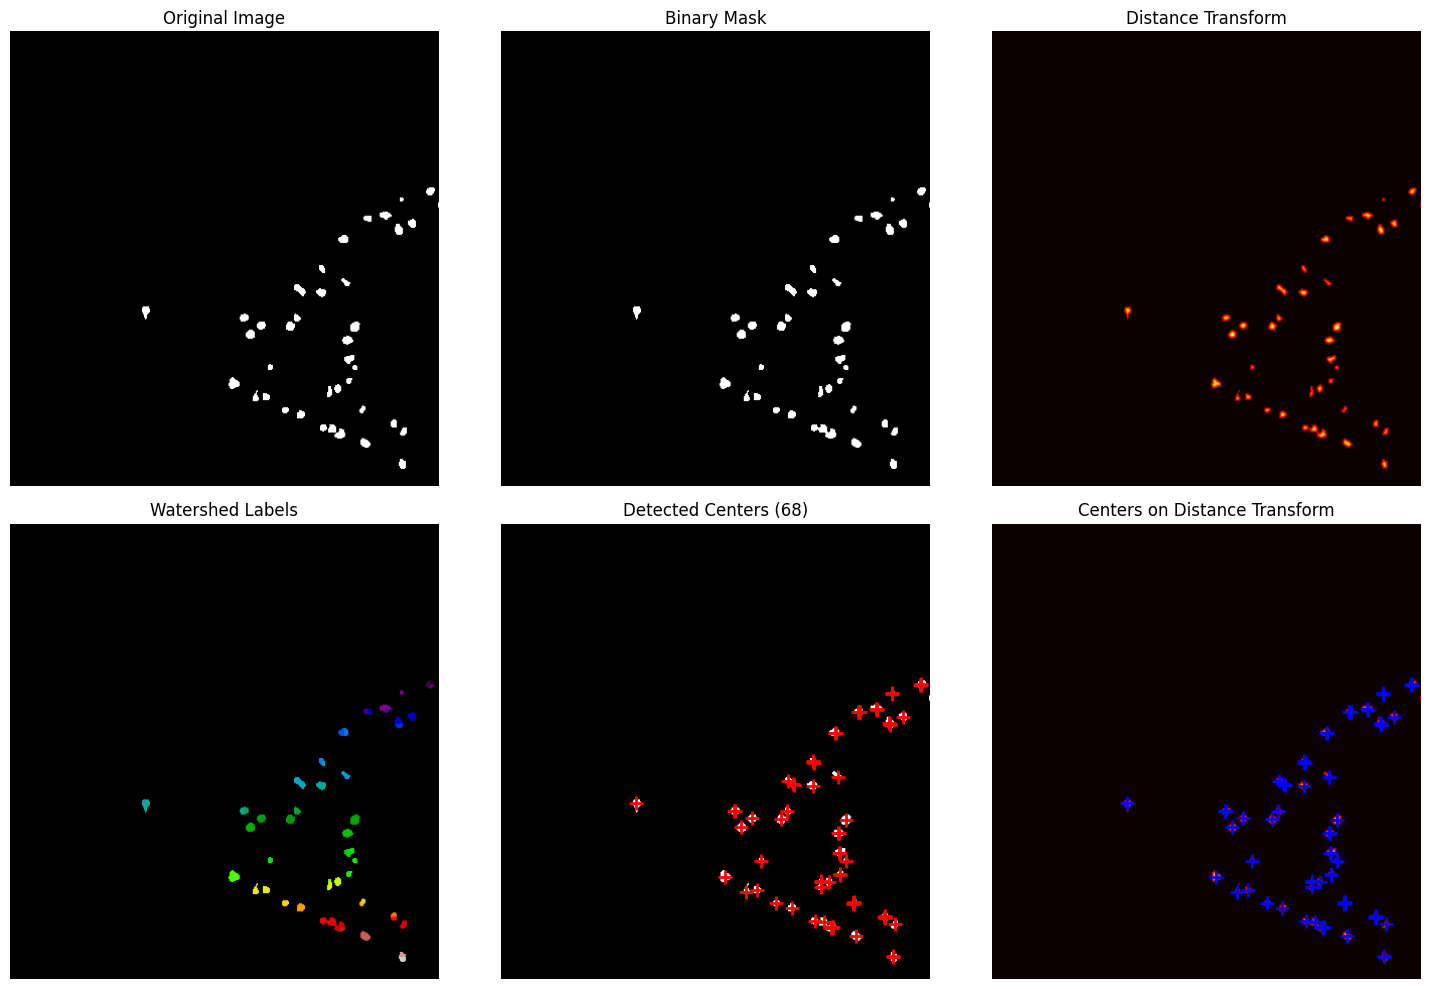
\includegraphics[width=0.95\textwidth]{figures/18_spine_prompt_training.png}
\captionof{figure}{Figure shows the process of finding positive prompts points from spines masks. Spine Centers are found using distance transform, connected spines are separated using watershed labels, combined together forms the positive prompts for the model. Scale: $0.94\,\mu\text{m}/\text{px}$}
\label{fig:spine_training_prompts}
\end{center}

\paragraph{Inference-Time Prompt Strategy}

During inference, spine locations are either detected automatically from \textit{Spine Detection Module} or added manually were used directly as positive prompts. \autoref{fig:tube_data} shows an example of detected spines across two patches. Each 3D coordinate was projected into 2D frames and fed into the \gls{SAMv2} prompt encoder without modification, maintaining consistency with the training distribution. For manual annotations, the \texttt{SpineTracker} extended prompts across adjacent frames to capture anisotropic spines. This unified, point-based strategy enabled the model to generate focused spine masks with high spatial precision.

\subsubsection{\textbf{Evaluation}}
Similar to the dendrite segmentation, the spine segmentation model was evaluated on a fixed validation split from the dataset, strictly excluding benchmark stacks. Every 500 iterations during training, validation was performed over 20 batches, each comprising 128$\times$128 patches without augmentation to ensure consistency. Predictions were thresholded at 0.5 after sigmoid activation and performance was quantified using the Dice coefficient and \gls{IoU} metrics.

Among all trained variants, the \texttt{\gls{SAMv2}-small} model at 128 resolution consistently achieved the best trade-off between speed and performance. Larger models and higher resolutions showed marginal improvements in Dice and \gls{IoU} but introduced considerable memory and runtime overhead without yielding biologically relevant benefits. The final selected model achieved stable performance with fast inference, making it suitable for integration into interactive annotation workflows.

\subsubsection{\textbf{Integration into Neuro-\gls{SAM} Pipeline}}
The spine segmentation model is tightly integrated into the Neuro-\gls{SAM} workflow. After spine candidates are confirmed, 128$\times$128 patches are extracted around each spine and processed using the fine-tuned \texttt{\gls{SAMv2}-small} model. Foreground prompts are derived from spine centers, with optional dendrite-based suppression.

The model handles segmentation and post-processing internally. Overlapping predictions are merged adaptively and visualized directly in the Napari viewer, with contrasting colors for clarity. Each segmented spine is rendered with a high-contrast color and users can interactively inspect, correct, or export the final results. This tightly coupled design ensures that spine segmentation is not a standalone operation, but rather a seamless continuation of the detection workflow anchored to biological structure and visual feedback.

The Neuro-\gls{SAM} pipeline brings together four tightly integrated modules: path tracing, dendrite segmentation, spine detection, and spine segmentation into a coherent and interactive system for annotating dendritic structures in 3D microscopy volumes. Each module operates independently but communicates contextual signals to maintain spatial and semantic consistency. By combining foundation models like \texttt{\gls{SAMv2}} with patch-wise inference, custom prompt logic, and real-time interaction, the system achieves fine-grained, high-fidelity predictions with minimal manual input.

With the technical foundations in place and the modular design firmly established, the discussion now shifts toward empirical evaluation. The next section focuses on how these methods perform in practice, analyzing their quantitative accuracy, robustness across datasets, and overall annotation efficiency.


        \chapter{Results}

This chapter presents a comprehensive evaluation of Neuro-\gls{SAM} and its constituent foundation model variants across the tasks of path tracing, dendrite segmentation, and dendritic spine segmentation. Building upon the modular architecture described in the Feature Work chapter, our goal is to empirically validate the performance improvements introduced by integrating foundation models into the segmentation pipeline. All models were benchmarked against \gls{DeepD3} \cite{Fernholz_2024}, which serves as the baseline due to its strong community adoption, open accessibility, and multi-rater validation framework. Through quantitative comparisons on the benchmark dataset and qualitative analysis across diverse imaging conditions, we demonstrate the strengths and limitations of each model configuration, culminating in a robust evaluation of the proposed Neuro-\gls{SAM} framework.

\section{Evaluation Protocol}
To rigorously evaluate the performance of Neuro-\gls{SAM}, we established a unified benchmarking pipeline incorporating diverse microscopy datasets, standardized metrics, and consistent evaluation logic across all models and tasks. This section outlines the datasets used, the metrics computed, and the procedures adopted for testing Neuro-\gls{SAM}.

\subsection{Datasets}
All experiments were conducted on high-resolution 3D microscopy volumes, primarily centered around the \textit{benchmark dataset} \cite{Fernholz_2024}, which offers multi-rater annotations for both dendrites and dendritic spines. Additional experiments included curated datasets with varied voxel resolutions, imaging modalities, and fluorescent indicators to test generalizability.

\subsection{Evaluation Metrics}
Segmentation quality was assessed using pixel-wise and object-level metrics, computed separately for dendrites and spines:
\begin{itemize}
\item \textbf{Intersection-over-Union}: Quantifies the overlap between predicted and ground truth masks. The \gls{IoU} can be formulated as :

\[
IoU = \frac{|P \cap G|}{|P \cup G|}
\]

where $P$ and $G$ denote the sets of predicted and ground truth foreground pixels, respectively.
\item \textbf{Dice Score}: Measures segmentation similarity, balancing precision and recall. Meanwhile the Dice Score can be computed as:

\[
Dice = \frac{2 |P \cap G|}{|P| + |G|}
\]

\item \textbf{Recall}: Fraction of ground truth instances detected by the model.
\item \textbf{Precision}: Fraction of predicted instances that correspond to true positives.
\end{itemize}

All metrics were computed on the maximum intensity projection of the dataset. In the following section, we first revisit the baseline performance of \gls{DeepD3} to contextualize the comparative evaluation.

\section{Baseline: DeepD3 Performance Overview}
To establish a consistent baseline for evaluating the segmentation performance of Neuro-\gls{SAM}, we re-ran the official \texttt{\gls{DeepD3}\_32F} model on the benchmark dataset \cite{Fernholz_2024}. \autoref{fig:deepd3_max_proj} shows a maximum intensity projection of the 3D input stack (top), along with \gls{DeepD3}'s predicted dendrite (middle) and spine (bottom) masks. As visualized, the dendrites are largely continuous and well-defined, while the spine predictions densely follow dendritic shafts, capturing a wide variety of spine shapes and sizes. However, occasional over-segmentation and background noise are also evident, particularly in regions with weak signal or closely packed structures.



\begin{center}
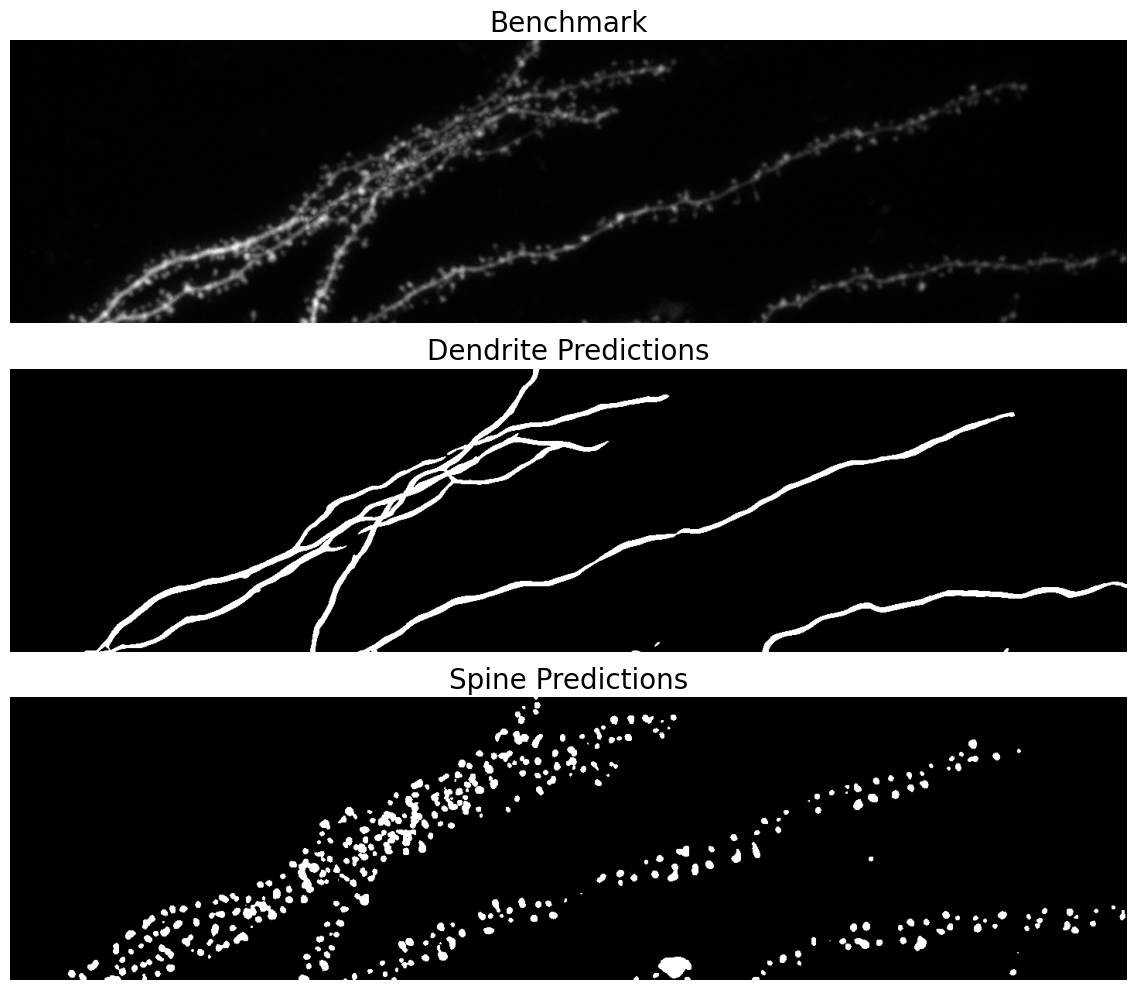
\includegraphics[width=0.7\textwidth]{figures/20_deepd3_max.png}
\captionof{figure}{\gls{DeepD3} prediction masks on the benchmark dataset. Top: Maximum intensity projection of the raw 3D microscopy stack. Middle: Dendrite prediction mask generated by the \gls{DeepD3}\_32F model. Bottom: Spine prediction mask from the same model. Scale: $0.94\,\mu\text{m}/\text{px}$}
\label{fig:deepd3_max_proj}
\end{center}

To quantify \gls{DeepD3}’s performance, predictions were compared against three expert raters (U, V, W), as well as their intersection and union masks. The full evaluation metrics Dice, \gls{IoU}, Precision, and Recall are summarized in \autoref{tab:deepd3_metrics}, with corresponding visualizations shown in \autoref{fig:deepd3_dice_iou} and \autoref{fig:deepd3_prec_recall}. For dendrites, the Dice scores range from 0.741 to 0.824 across individual raters, and 0.723 and 0.820 for the intersection and union masks, respectively. The corresponding \gls{IoU} values range from 0.416 to 0.609. In spine segmentation, \gls{DeepD3} achieves Dice scores as high as 0.775 (intersection) and 0.757 (rater W), but performance degrades when evaluated against union masks, where the \gls{IoU} drops to 0.545. This reflects the model's high specificity but occasional miss of borderline spines. 


\begin{table}[caption={Dice, \gls{IoU}, Precision, and Recall scores for dendrites and spines across raters, intersection, and union of \gls{DeepD3}.}, label=tab:deepd3_metrics]
\centering
\scriptsize
    \begin{tabular}{c c c c c c c}
        \toprule
        {\bf Rater / Consensus} & {\bf Dice Dendrites} & {\bf \gls{IoU} Dendrites} & {\bf Dice Spines} & {\bf \gls{IoU} Spines} & {\bf Precision Spines} & {\bf Recall Spines} \\ \midrule
            U & 0.815 & 0.688 & 0.587 & 0.416 & 0.632 & 0.899 \\
            V & 0.824 & 0.701 & 0.594 & 0.423 & 0.573 & 0.916 \\
            W & 0.741 & 0.589 & 0.757 & 0.609 & 0.738 & 0.850 \\
            Intersection & 0.723 & 0.775 & 0.633 & 0.519 & 0.735 & 0.850 \\
            Union & 0.820 & 0.472 & 0.545 & 0.375 & 0.455 & 0.869 \\
        \midrule
    \end{tabular}
\end{table}

\begin{center}
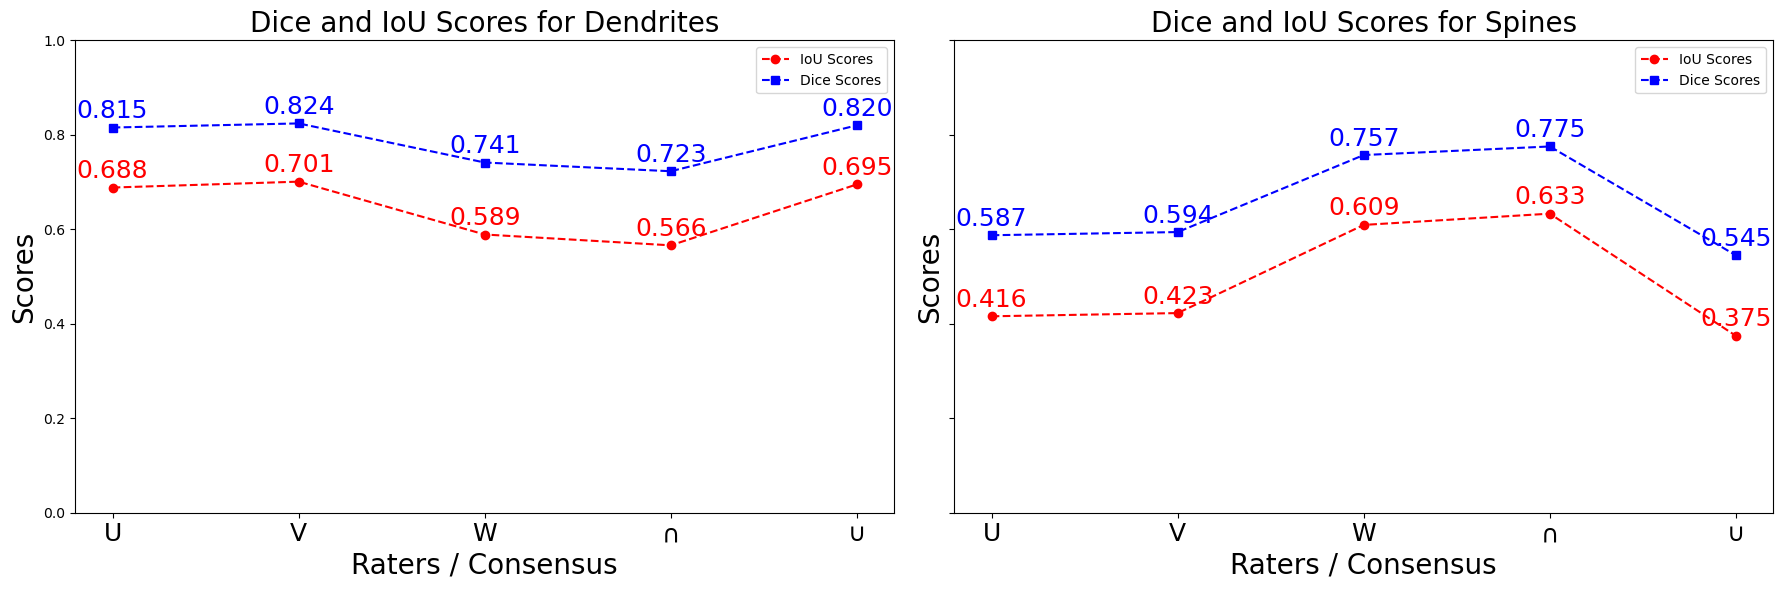
\includegraphics[width=0.95\textwidth]{figures/21_deepd3_dice_iou.png}
\captionof{figure}{Quantitative performance of \gls{DeepD3} against individual raters and consensus masks. Left: Dice and \gls{IoU} scores for dendrite segmentation across raters U, V, W, as well as intersection and union masks. Right: Dice and \gls{IoU} scores for spine segmentation using the same evaluation setup. Scale: $0.94\,\mu\text{m}/\text{px}$}
\label{fig:deepd3_dice_iou}
\end{center}

Precision and recall values further highlight the model’s detection tendencies. As shown in \autoref{fig:deepd3_prec_recall}, recall remains consistently high across all raters, peaking at 0.916 (rater V) and staying above 0.85 in all cases. Precision, however, varies more substantially, dropping to 0.455 against the union mask indicating that while the model successfully captures the majority of annotated spines, it also predicts additional structures not present in the ground truth.

\begin{center}
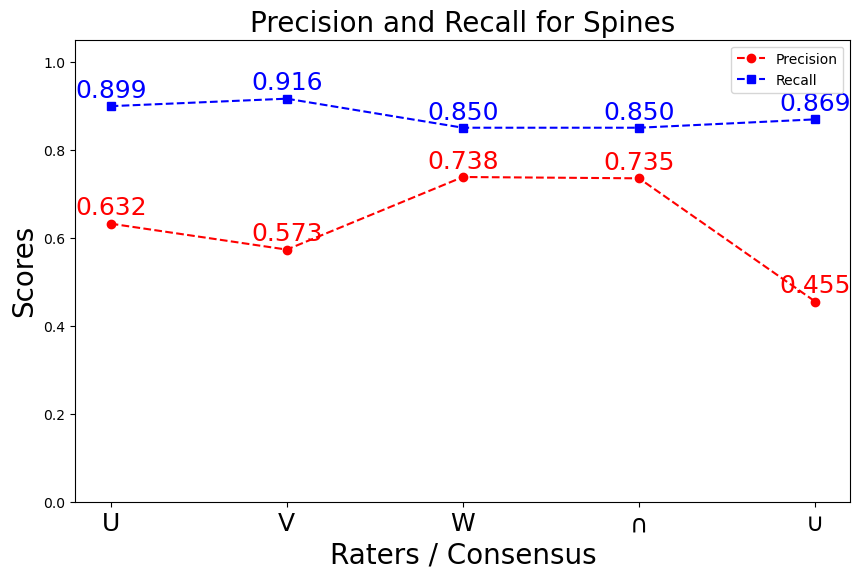
\includegraphics[width=0.7\textwidth]{figures/22_deepd3_prec_recall.png}
\captionof{figure}{Precision and recall of \gls{DeepD3} spine predictions. Recall remains consistently high across all raters and consensus masks, while precision varies more substantially, especially when evaluated against the union mask.}
\label{fig:deepd3_prec_recall}
\end{center}

A qualitative comparison between \gls{DeepD3}'s predictions and the expert annotations is shown in \autoref{fig:deepd3_qualitative}. While the dendrite predictions appear morphologically consistent across most raters, the spine segmentations reveal subtle differences in density and placement. Rater W, for example, tends to annotate fewer spines compared to raters U and V. The intersection mask highlights only a conservative core set of spines, whereas the union mask introduces substantial variability, including ambiguities at dendrite intersections or low-contrast areas. These visualizations provide a concrete reference for understanding both the strengths and limitations of \gls{DeepD3} as a baseline for comparative evaluation.

\begin{center}
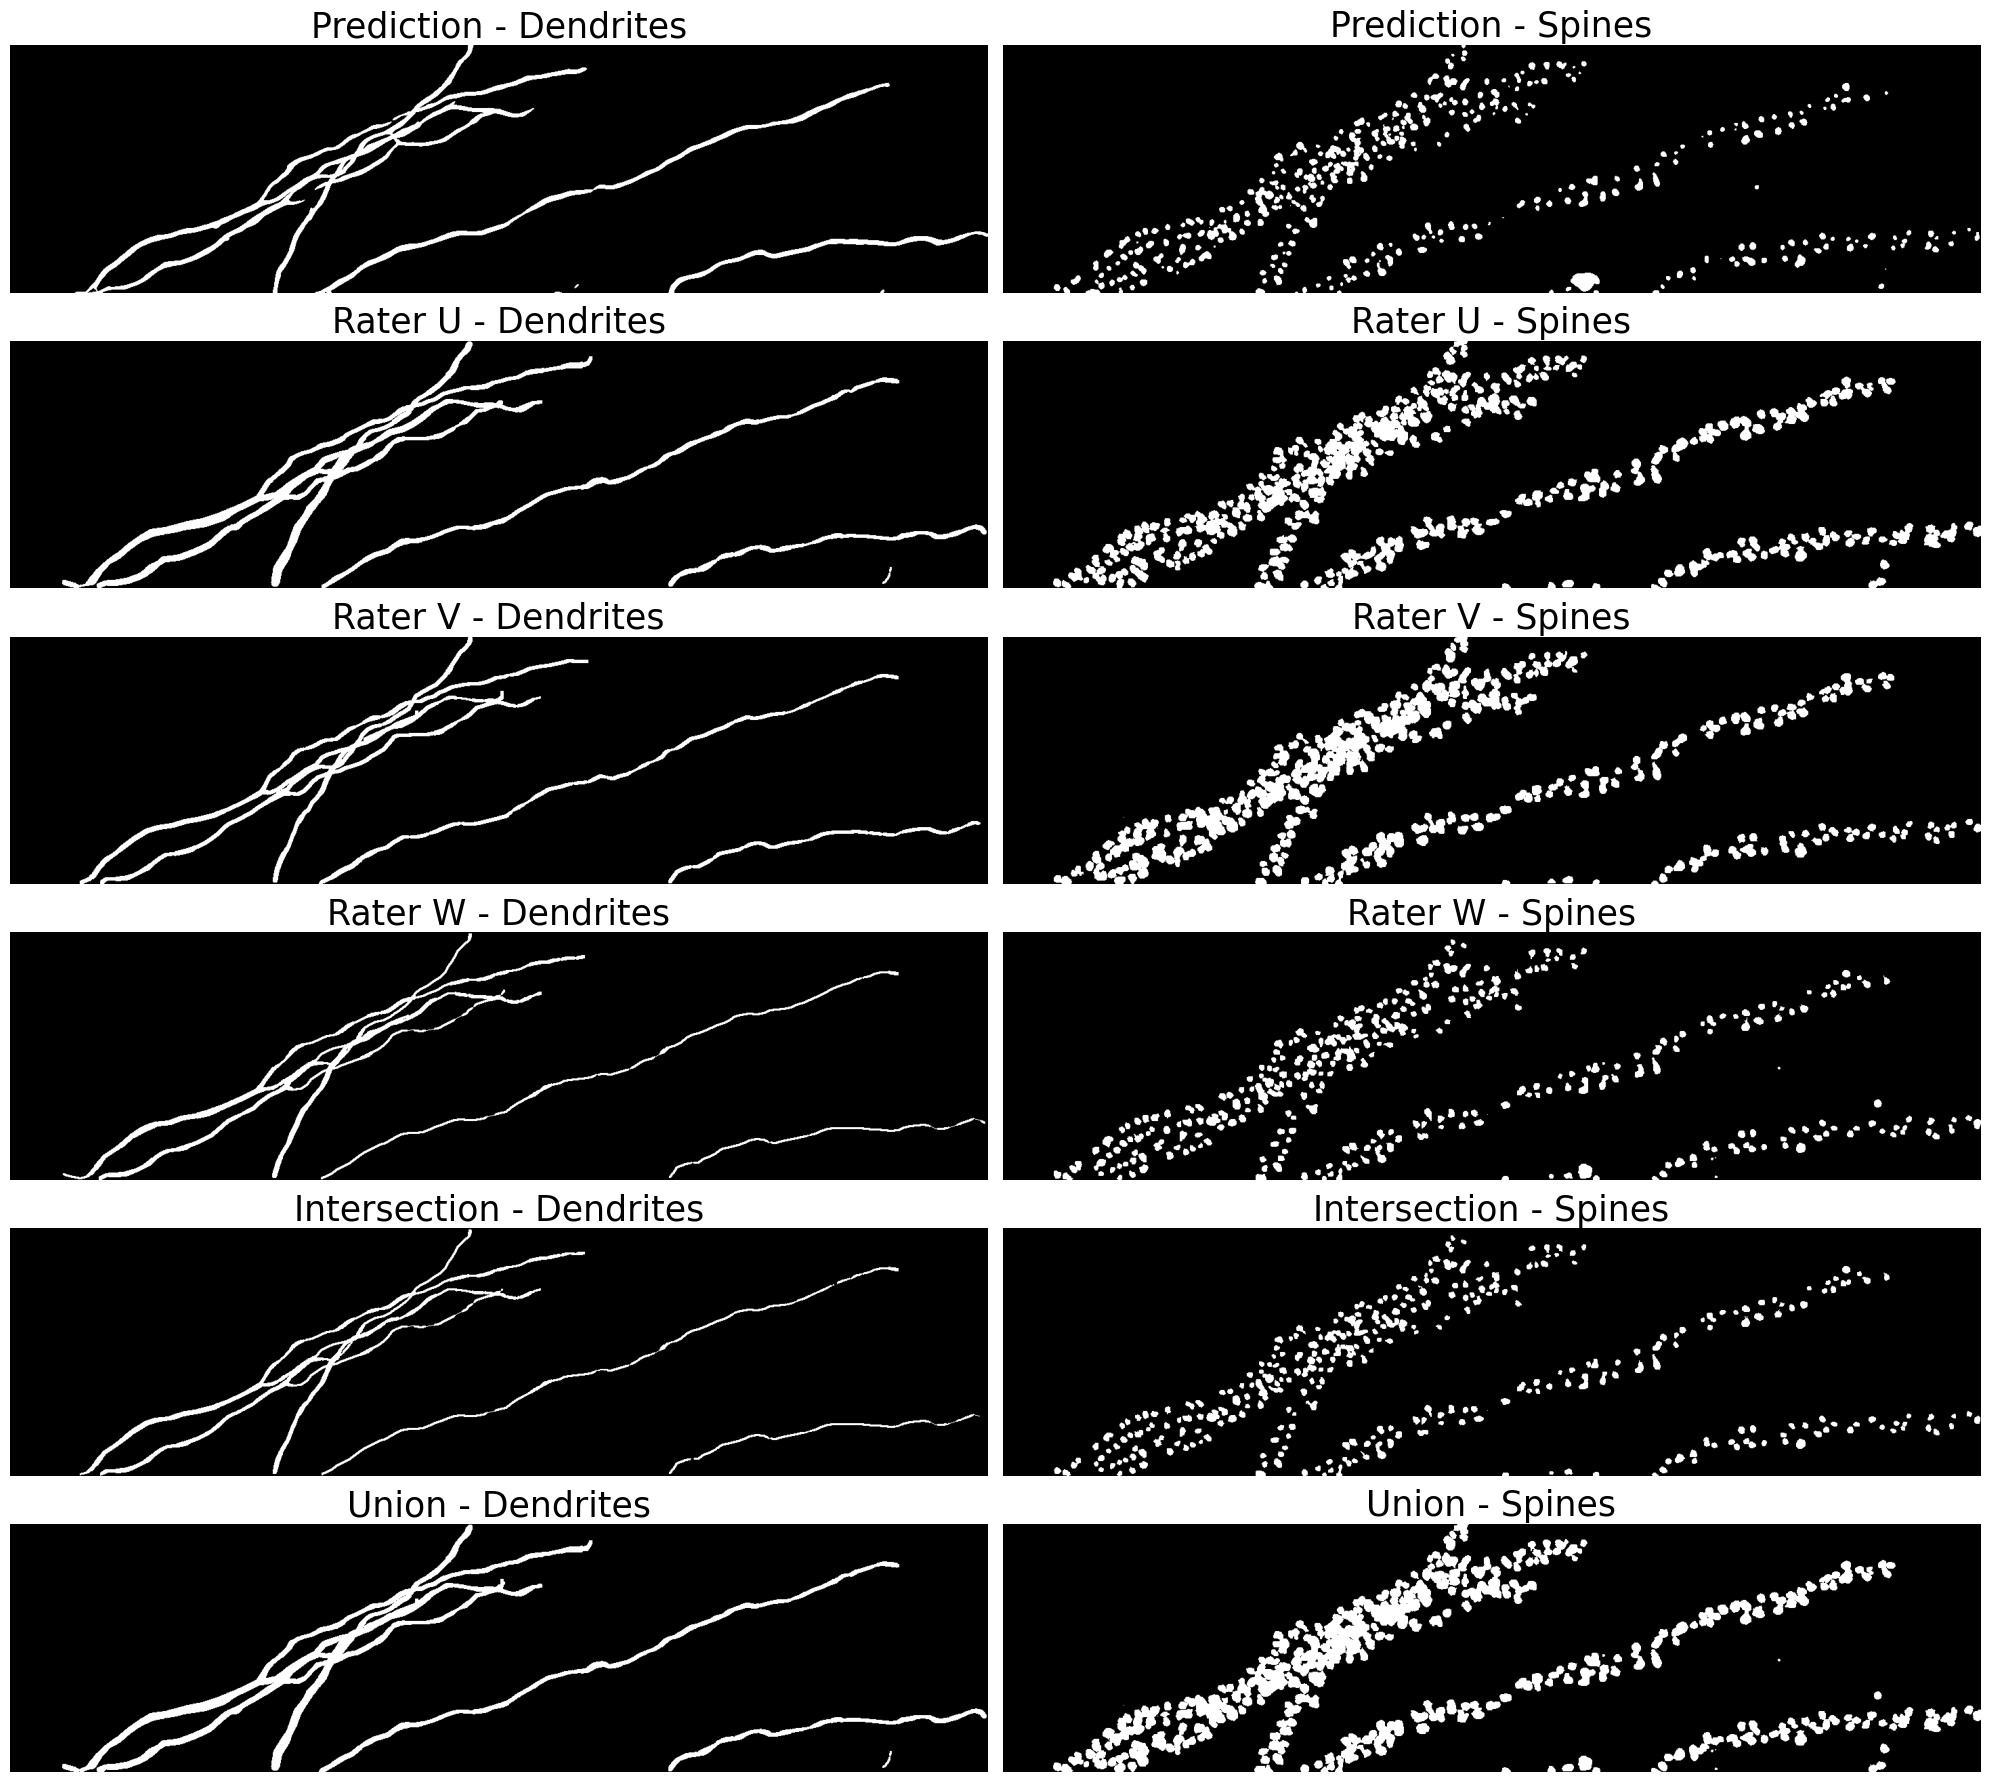
\includegraphics[width=0.95\textwidth]{figures/23_deepd3_qualitative.png}
\captionof{figure}{Qualitative comparison of \gls{DeepD3} predictions with individual rater annotations. Rows show the predicted masks, rater U, V, and W annotations, as well as intersection and union consensus masks. While dendrite predictions closely align across all references, spine annotations show notable differences in density and coverage. Scale: $0.94\,\mu\text{m}/\text{px}$}
\label{fig:deepd3_qualitative}
\end{center}

These results establish a strong empirical baseline for both dendrite and spine segmentation. In the following section, we evaluate the performance of \gls{SAM}-based approaches introduced in the Feature Work chapter.

\section{Segment Anything Model}
The \gls{SAM} model was evaluated on the benchmark dataset in both zero-shot and fine-tuned settings. Given its general-purpose design, \gls{SAM} was applied only to the task of \textit{dendrite segmentation}. For zero-shot inference, we used a grid-based prompting strategy, placing point prompts at regular intervals across the image plane. For fine-tuning, \gls{SAM} was tested using point prompts derived from \texttt{goodFeaturesToTrack} along the dendritic shaft, with overlapping patches extracted from the training volumes. All results presented in this section were obtained using the \texttt{\gls{ViT}-H} variant of \gls{SAM}.

A qualitative comparison of the raw benchmark stack, zero-shot predictions (grid size 16), and fine-tuned predictions is shown in \autoref{fig:sam_qualitative}. The zero-shot predictions exhibit sparse, patchy coverage and substantial noise. While some dendritic structures are partially identified, the segmentation lacks continuity and misses finer branches entirely. In contrast, the fine-tuned model produces denser masks with greater coverage of dendrite segments, though it still suffers from over-segmentation and grid-like artifacts related to patch-based inference.

\begin{center}
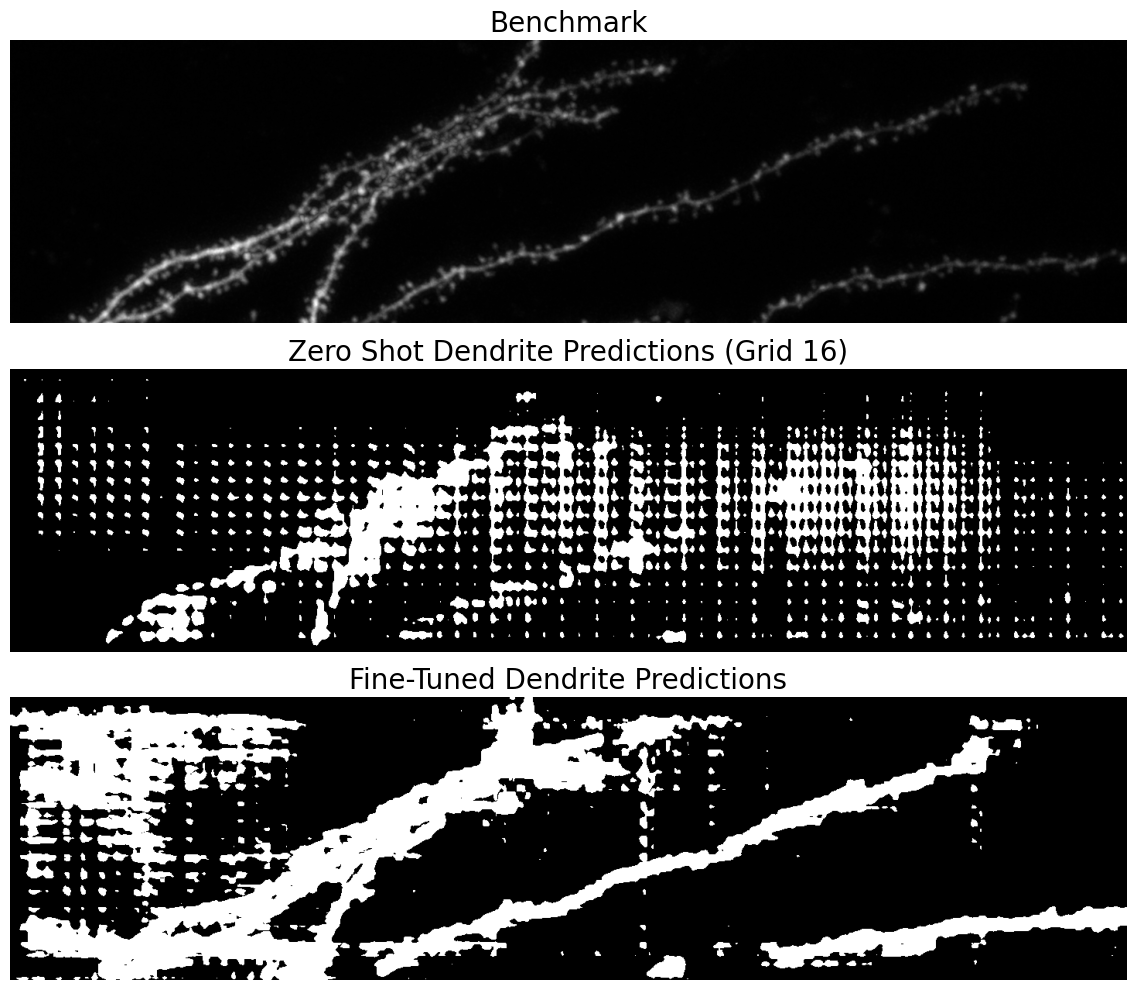
\includegraphics[width=0.8\textwidth]{figures/24_sam_qualitative.png}
\captionof{figure}{Qualitative comparison of \gls{SAM} predictions. Top: Raw benchmark image. Middle: Zero-shot prediction using grid size 16. Bottom: Prediction from fine-tuned \gls{SAM}. Zero-shot output is sparse and noisy, while fine-tuned results improve coverage but remain over-segmented. Scale: $0.94\,\mu\text{m}/\text{px}$}
\label{fig:sam_qualitative}
\end{center}

Quantitative results for the zero-shot \gls{SAM} setup are shown in \autoref{fig:sam_zeroshot_metrics}. Using grid-based point prompts, the best performance was observed at a grid size of 16, with a Dice score of 0.248 and an \gls{IoU} of 0.141 against rater U. At coarser grid sizes (32 and above), the model failed to produce any coherent segmentation, yielding near-zero scores. This poor performance can be attributed to the fact that grid prompts are spatially uniform and semantically uninformed. Since \gls{SAM} relies heavily on prompt relevance to generate accurate masks, indiscriminate prompting across the image leads to fragmented and noisy outputs, especially in dense and ambiguous biomedical scenes like dendrites.

\begin{center}
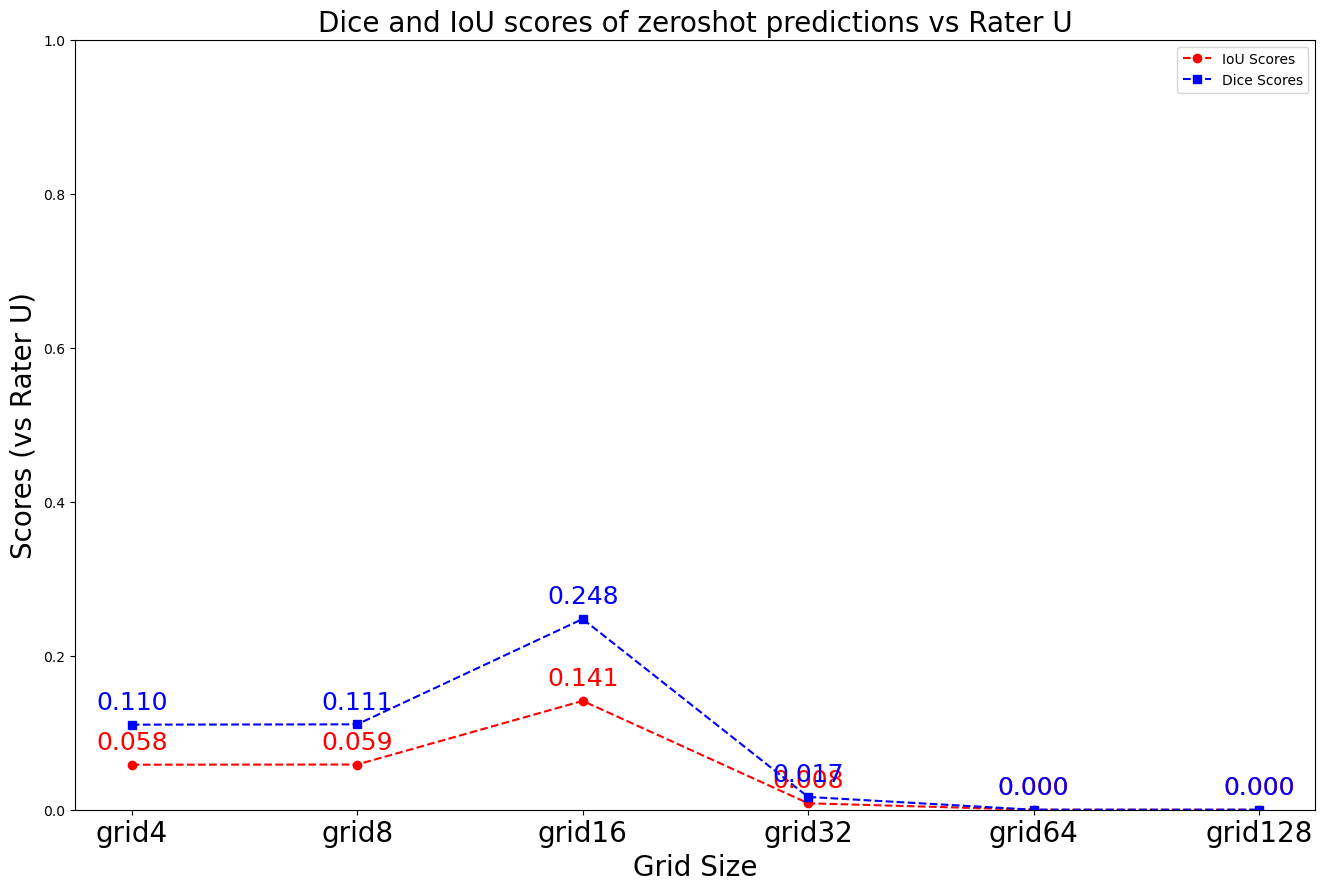
\includegraphics[width=0.8\textwidth]{figures/25_sam_zeroshot_metrics.png}
\captionof{figure}{Zero-shot \gls{SAM} dendrite segmentation performance. Dice and \gls{IoU} scores across different grid sizes using grid-based point prompts, evaluated against rater U. Performance peaks at grid size 16, but remains very bad overall, highlighting the ineffectiveness of prompt-agnostic zero-shot inference for this task.}
\label{fig:sam_zeroshot_metrics}
\end{center}

To address these limitations, the model was fine-tuned on task-specific dendritic data using tracked feature points as prompts. As shown in \autoref{fig:sam_finetuned_metrics}, fine-tuning substantially improved segmentation quality. The highest Dice and \gls{IoU} scores were observed against the union mask, reaching 0.341 and 0.205, respectively. Performance dropped when compared with intersection mask, where Dice and \gls{IoU} fell to 0.203 and 0.113. This spread reflects the continued sensiti\gls{ViT}y of the model to prompt quality and ground truth ambiguity. While fine-tuning helped the model learn contextual cues and reduced noise, the predictions still exhibited grid artifacts and lacked precision around dendritic boundaries. Nevertheless, the improvement over the zero-shot variant establishes the importance of task-specific adaptation even for powerful foundation models like \gls{SAM}.

\begin{center}
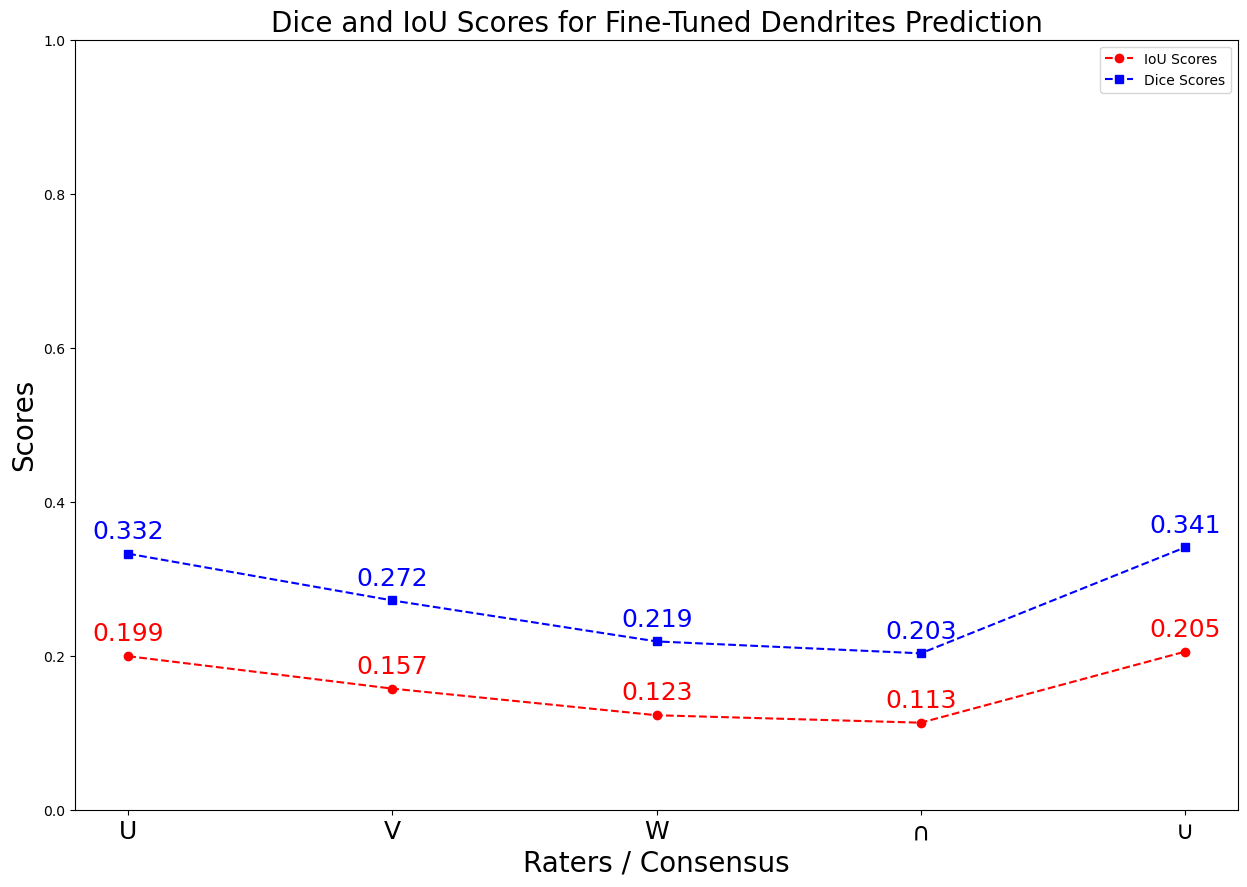
\includegraphics[width=0.8\textwidth]{figures/26_sam_finetuned_metrics.png}
\captionof{figure}{Fine-tuned \gls{SAM} dendrite segmentation performance. Dice and \gls{IoU} scores evaluated against three individual raters and consensus masks. Fine-tuning improves performance substantially over zero-shot \gls{SAM}, though results still vary depending on the reference mask.}
\label{fig:sam_finetuned_metrics}
\end{center}

These results demonstrate that while \gls{SAM} possesses general segmentation capabilities, it fails to perform reliably on dendritic structures without task-specific adaptation. Fine-tuning improves segmentation quality but remains insufficient for precise and consistent dendrite segmentation. This motivated the exploration of parameter-efficient fine-tuning strategies such as Low Rank Adaptation.

\section{SAM with Low-Rank Adaptation}
While the fine-tuned \gls{SAM} model showed moderate improvements over zero-shot performance, its outputs remained noisy and prone to over-segmentation. To improve generalization while maintaining training efficiency, we leveraged \gls{LoRA} to fine-tune \gls{SAM} on the dendrite segmentation task. \gls{LoRA} introduces task-specific trainable matrices into frozen transformer weights, significantly reducing the number of learnable parameters while preserving model capacity. Based on the failure of prompt-agnostic zero-shot \gls{SAM}, we directly adopted a fine-tuned \gls{LoRA} setup, avoiding zero-shot evaluation entirely.

A qualitative example comparing the benchmark image and \gls{SAM} + \gls{LoRA} predictions is shown in \autoref{fig:lora_qualitative}. Compared to both zero-shot and fully fine-tuned \gls{SAM}, \gls{LoRA} predictions demonstrate stronger continuity along dendritic shafts, reduced noise, and better adherence to structural boundaries. Visual artifacts observed in earlier variants, such as over-segmentation and patch-induced grid effects, are substantially minimized.

\begin{center}
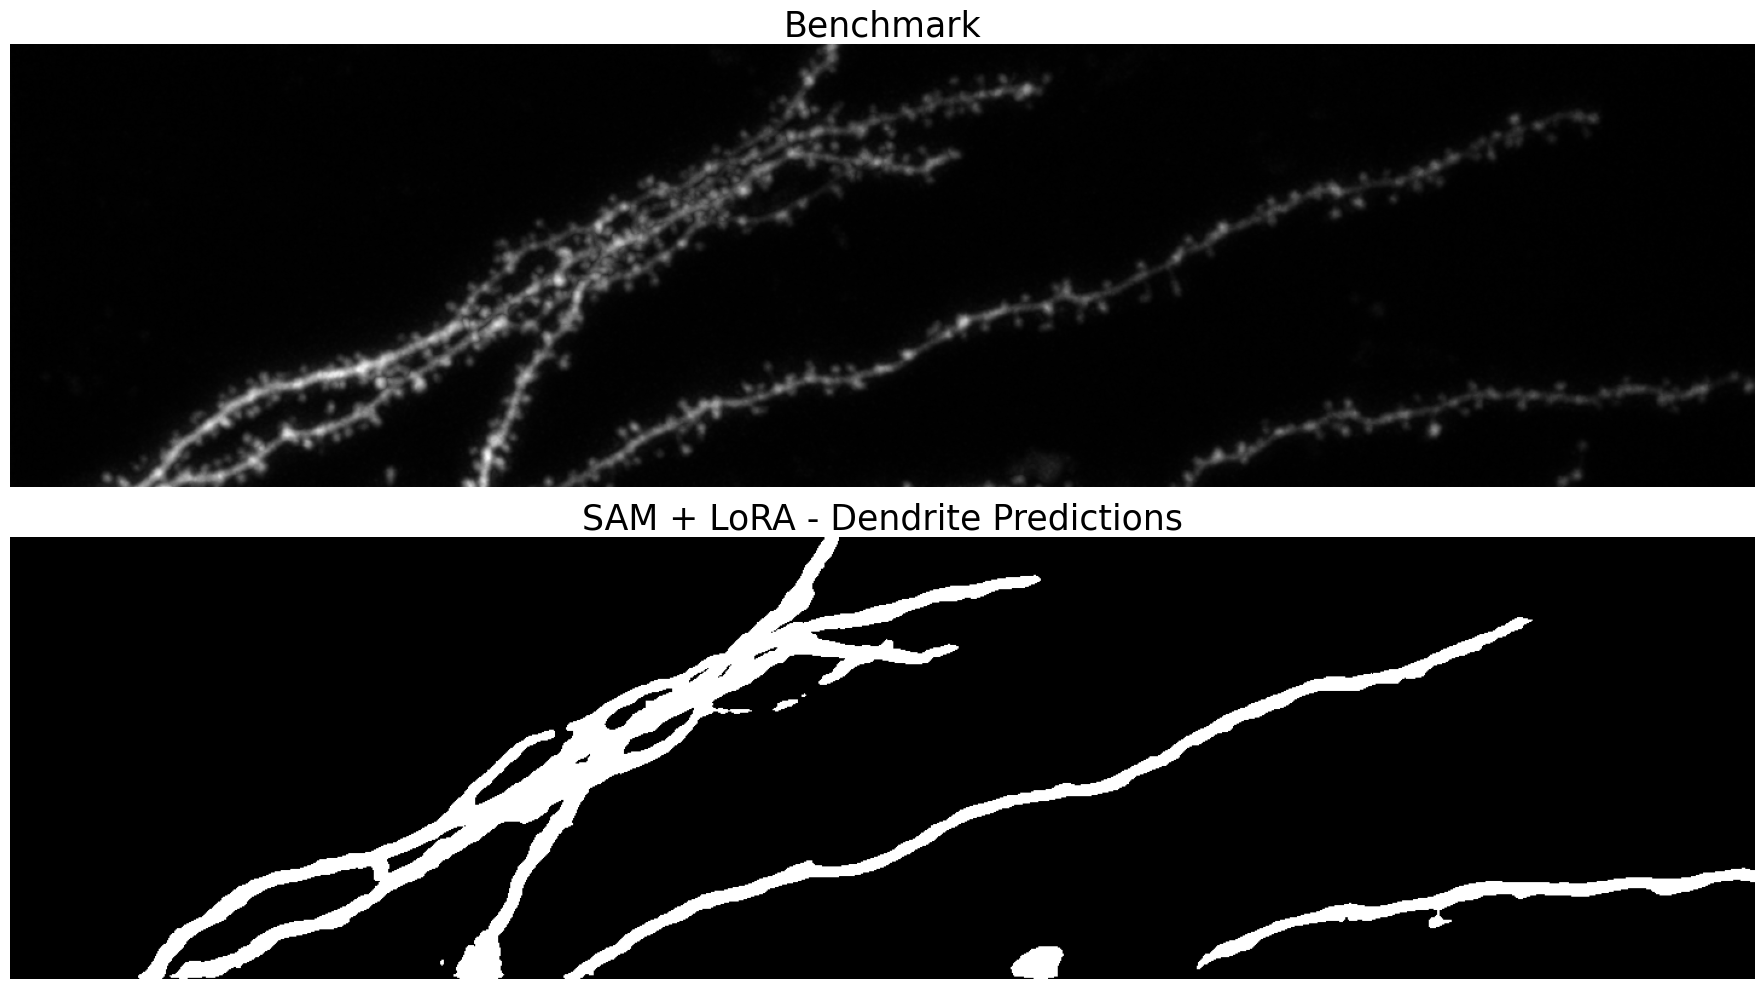
\includegraphics[width=0.9\textwidth]{figures/27_lora_qualitative.png}
\captionof{figure}{Qualitative dendrite segmentation using \gls{SAM} + \gls{LoRA}. Top: Raw benchmark image. Bottom: Prediction using \gls{SAM} + \gls{LoRA}. The model produces clean, continuous segmentation masks with reduced background noise and improved shaft delineation. Scale: $0.94\,\mu\text{m}/\text{px}$}
\label{fig:lora_qualitative}
\end{center}

\begin{center}
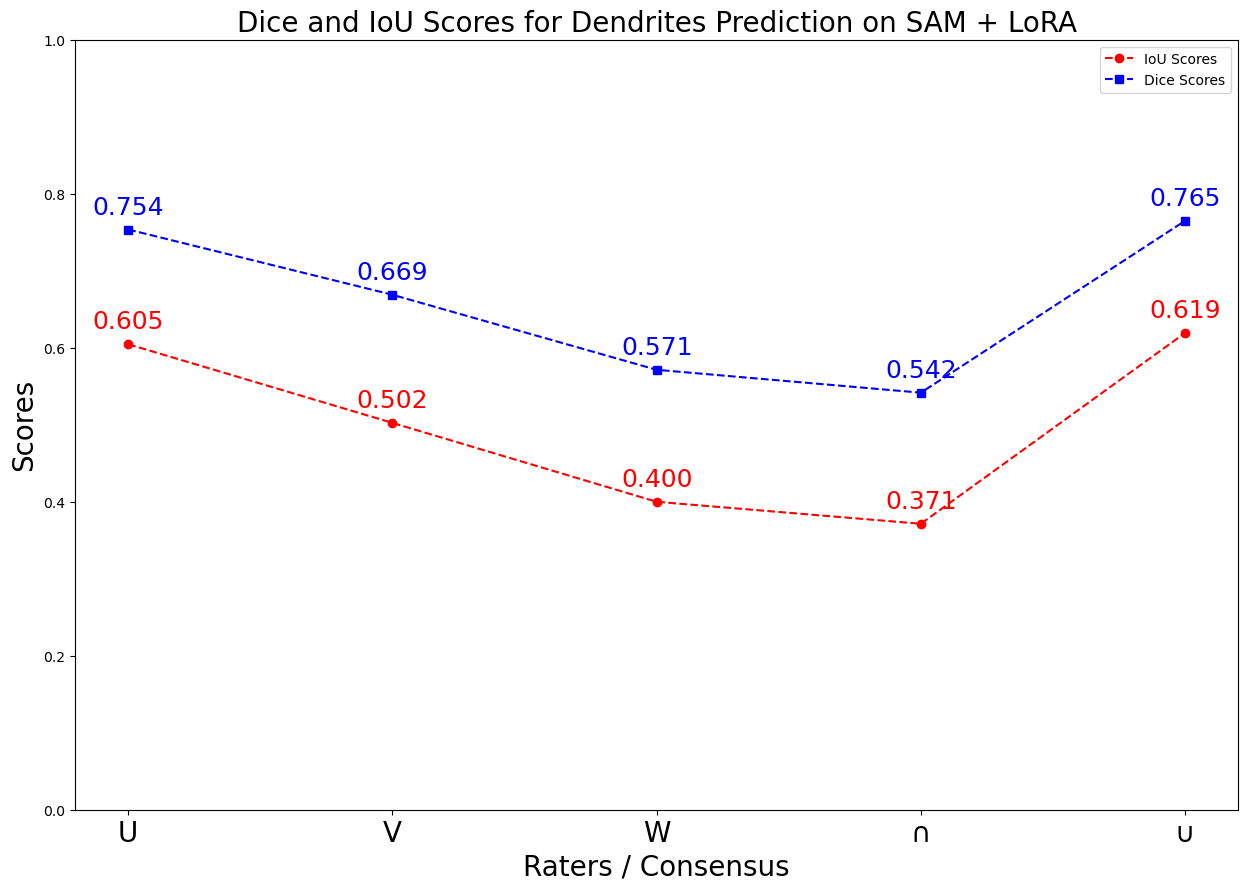
\includegraphics[width=0.8\textwidth]{figures/28_lora_metrics.png}
\captionof{figure}{Dice and \gls{IoU} scores for \gls{SAM} + \gls{LoRA} dendrite segmentation. Evaluation against individual raters and consensus masks. \gls{LoRA} shows consistent improvements over both zero-shot and fully fine-tuned \gls{SAM}. Scale: $0.94\,\mu\text{m}/\text{px}$}
\label{fig:lora_metrics}
\end{center}


Quantitatively, \gls{SAM} + \gls{LoRA} outperforms both the zero-shot and fully fine-tuned \gls{SAM} variants across all raters and consensus masks, as shown in \autoref{fig:lora_metrics}. The model achieves a maximum Dice score of 0.765 and \gls{IoU} of 0.619 when evaluated against the union mask. Even against stricter references such as the intersection mask, performance remains high, with Dice and \gls{IoU} scores of 0.542 and 0.371, respectively. These consistent improvements confirm that \gls{LoRA}-based fine-tuning enhances both mask quality and generalization without incurring the instability of full model training.

To further assess qualitative differences, we compared frame-level predictions across methods. \autoref{fig:lora_framewise_comparison} shows predictions for two representative slices (Frame 23 and 36). \gls{SAM} + \gls{LoRA} more accurately captures dendritic continuity and fine detail compared to \gls{DeepD3}, while also avoiding the patch-based artifacts that degraded \gls{SAM}’s outputs. These results reinforce \gls{LoRA}’s effectiveness in enabling stable, parameter-efficient fine-tuning tailored to the structural characteristics of dendrites.

\begin{center}
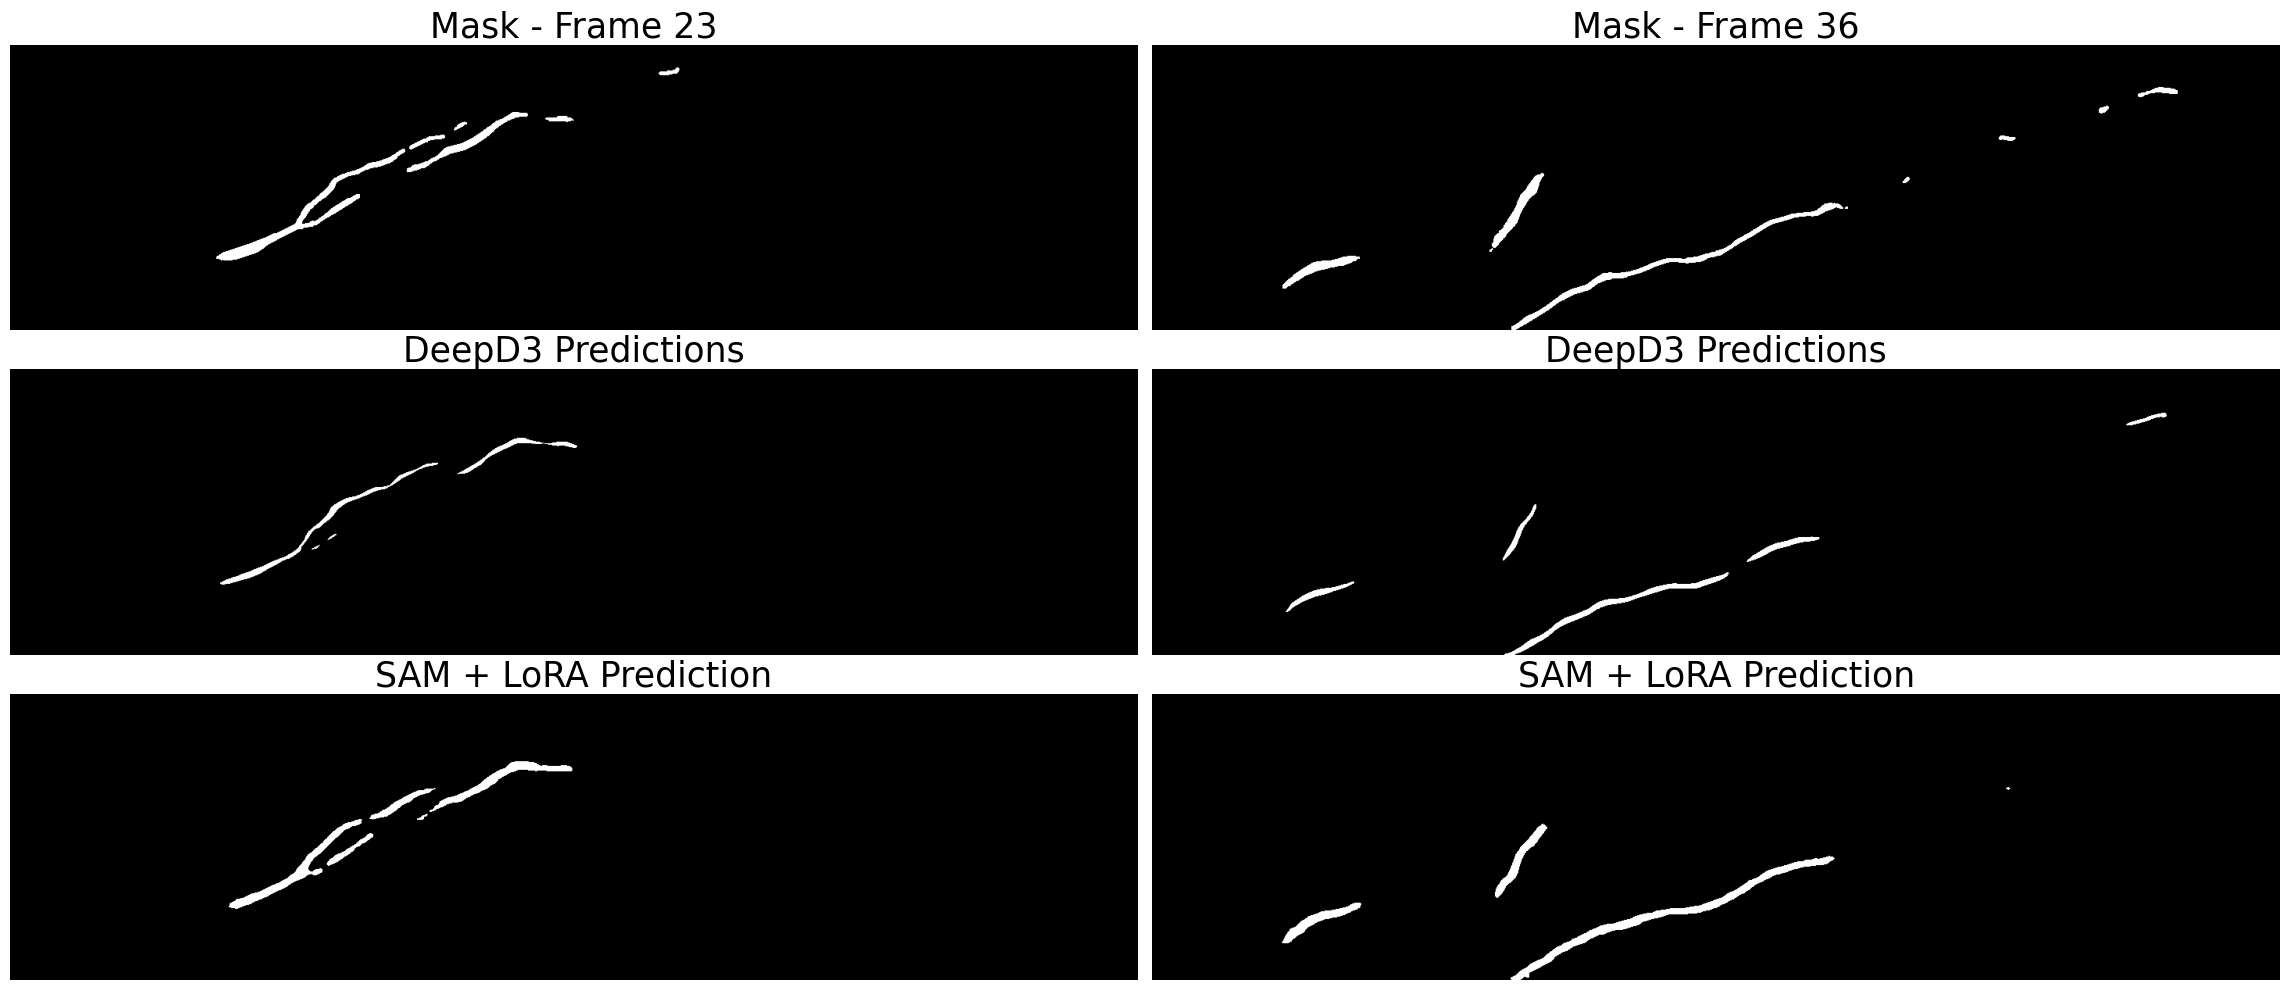
\includegraphics[width=0.95\textwidth]{figures/29_lora_framewise_comparison.png}
\captionof{figure}{Frame-wise comparison across models. Top: Ground truth masks for Frames 23 and 36. Middle: \gls{DeepD3} predictions. Bottom: \gls{SAM} + \gls{LoRA} predictions. \gls{LoRA} outputs display better structural continuity and less fragmentation than \gls{DeepD3}, and fewer artifacts than standard \gls{SAM}. Scale: $0.94\,\mu\text{m}/\text{px}$}
\label{fig:lora_framewise_comparison}
\end{center}

Overall, \gls{SAM}+\gls{LoRA} serves as a strong middle ground between zero-shot generalization and full-model fine-tuning, offering improved performance with fewer learnable parameters. These findings build a strong case for its use in domain-adapted segmentation pipelines, especially when working with limited annotations. Its balance of efficiency and accuracy makes \gls{SAM}+\gls{LoRA} particularly well-suited for neuroimaging tasks where dense annotations are costly. These advantages set the stage for our final and most comprehensive system: Neuro-\gls{SAM}.

\section{Neuro-SAM}
Neuro-\gls{SAM} is the final modular framework proposed in this thesis, designed to overcome the limitations observed in earlier \gls{SAM}-based approaches. Instead of building directly on previous variants like \gls{SAM} or \gls{SAM}+\gls{LoRA}, Neuro-\gls{SAM} leverages insights gained from those experiments to construct a more robust and task-specific pipeline powered by \gls{SAMv2}. The complete system consists of four interlinked modules: a waypoint-aware path tracing module, a \gls{SAMv2}-based dendrite segmentation module, a dual-view spine detection module, and a localized spine segmentation module. In this section, we evaluate the performance of each module independently, demonstrating the improvements achieved across dendrite and dendritic spine segmentation tasks.

\subsection{Path Tracing Module}
Accurate dendrite path tracing is a foundational step in Neuro-\gls{SAM}, enabling precise downstream segmentation and analysis. Manual tracing is both time-consuming and prone to subjective bias, particularly in dense or noisy regions. To address this, we developed a waypoint-aware path tracing module built upon a customized version of brightest-path-lib \cite{Jha_2023}. By allowing users to define start, end, and optional waypoint points, the module can robustly trace complex dendrite geometries with minimal input. This interactive tracing approach offers both control and automation, making it highly effective across a range of morphologies and image conditions.

\begin{center}
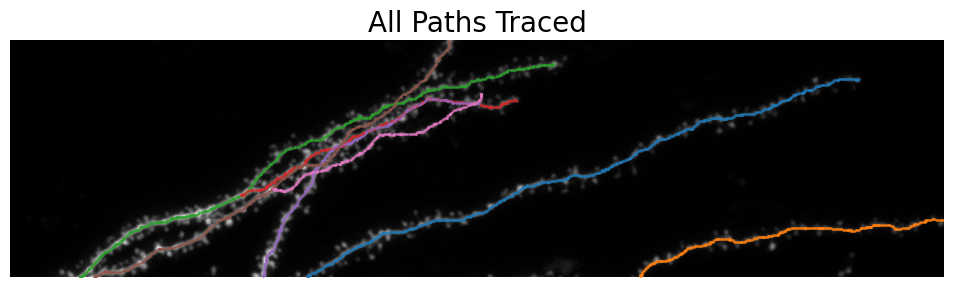
\includegraphics[width=1.0\textwidth]{figures/30_path_overview.png}
\captionof{figure}{Overview of traced dendritic paths. Multiple dendrites traced using the path tracing module of Neuro-\gls{SAM}. Each color represents an independently traced dendrite, demonstrating the module's robustness across diverse geometries and imaging conditions. Scale: $0.94\,\mu\text{m}/\text{px}$}
\label{fig:path_overview}
\end{center}

The path tracing module in Neuro-\gls{SAM} enables users to effortlessly trace complex dendritic structures by specifying just a start point, an end point, and optionally, a sparse set of waypoints. \autoref{fig:path_overview} illustrates a collection of traced dendritic paths over the benchmark stack, demonstrating the system's ability to handle diverse curvatures, crossings, and branch orientations. As shown in \autoref{fig:path_waypoints}, even challenging trajectories can be recovered with high spatial precision using minimal supervision. The waypoint-guided formulation allows flexible course correction in ambiguous regions, ensuring accurate adherence to the dendrite centerline without manual pixel-level editing. This capability not only streamlines user interaction but also produces reliable paths for downstream segmentation tasks.

\begin{center}
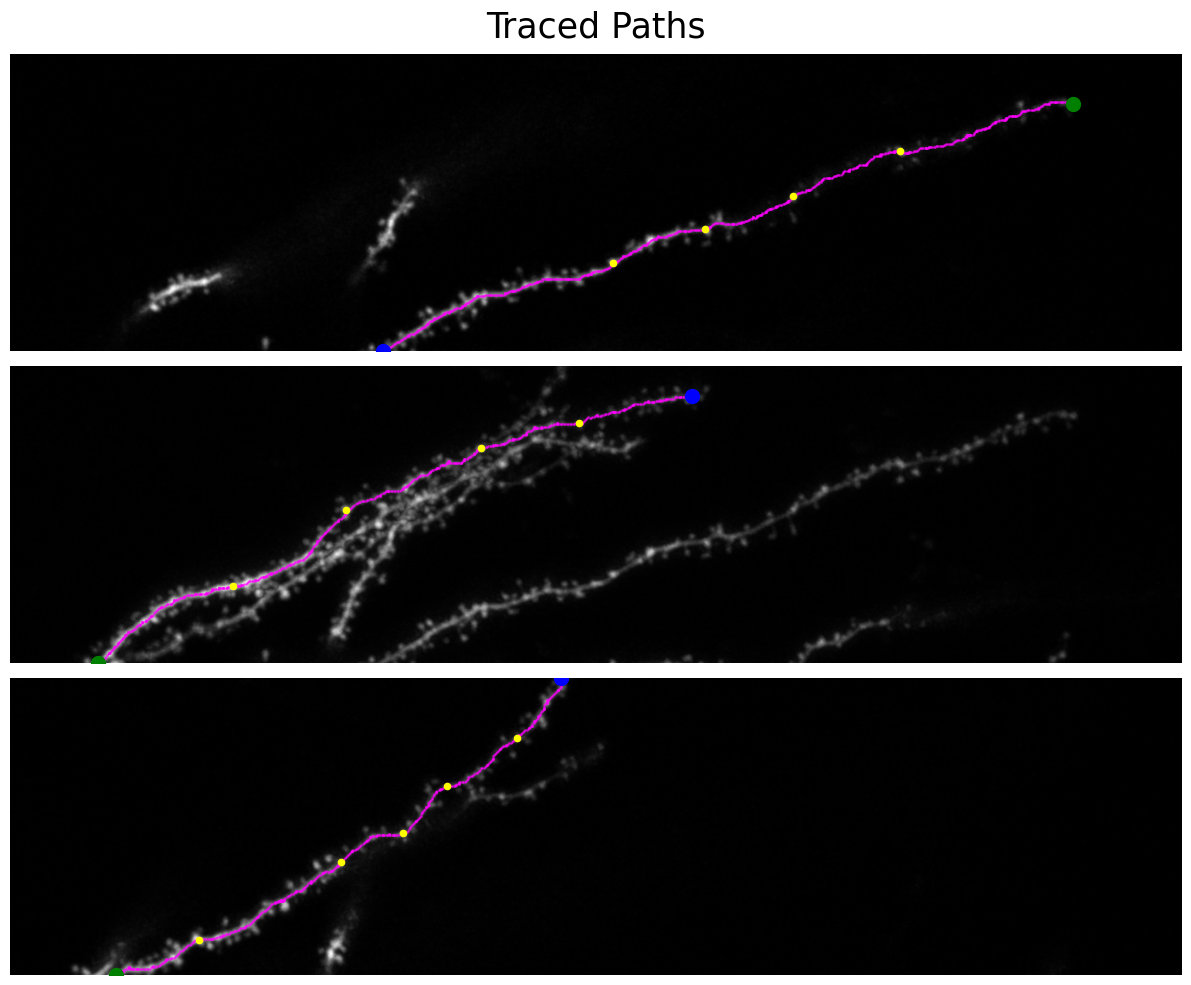
\includegraphics[width=0.8\textwidth]{figures/31_path_waypoints.png}
\captionof{figure}{Waypoint-guided path tracing. Example traces generated using the Neuro-\gls{SAM}'s path tracing module. Blue, green, and yellow dots represent start points, end points, and user-defined waypoints, respectively. Scale: $0.94\,\mu\text{m}/\text{px}$}
\label{fig:path_waypoints}
\end{center}

\subsubsection{\textbf{Comparison with brightest-path-lib}}
To evaluate the improvements introduced by our modified path tracing module, we compared its output to the original brightest-path-lib \cite{Jha_2023}, which computes optimal paths solely between two endpoints using voxel intensities. While the original method often produces valid traces in simple regions, it struggles in densely packed or twisted dendritic structures, frequently deviating from the true centerline or jumping across nearby branches. In contrast, Neuro-\gls{SAM}'s path tracing module provides local guidance at critical turning points, effectively constraining the search space and enabling more biologically plausible trajectories. Qualitatively, our module produces smoother, anatomically consistent paths with significantly fewer deviations or misroutes.

\begin{center}
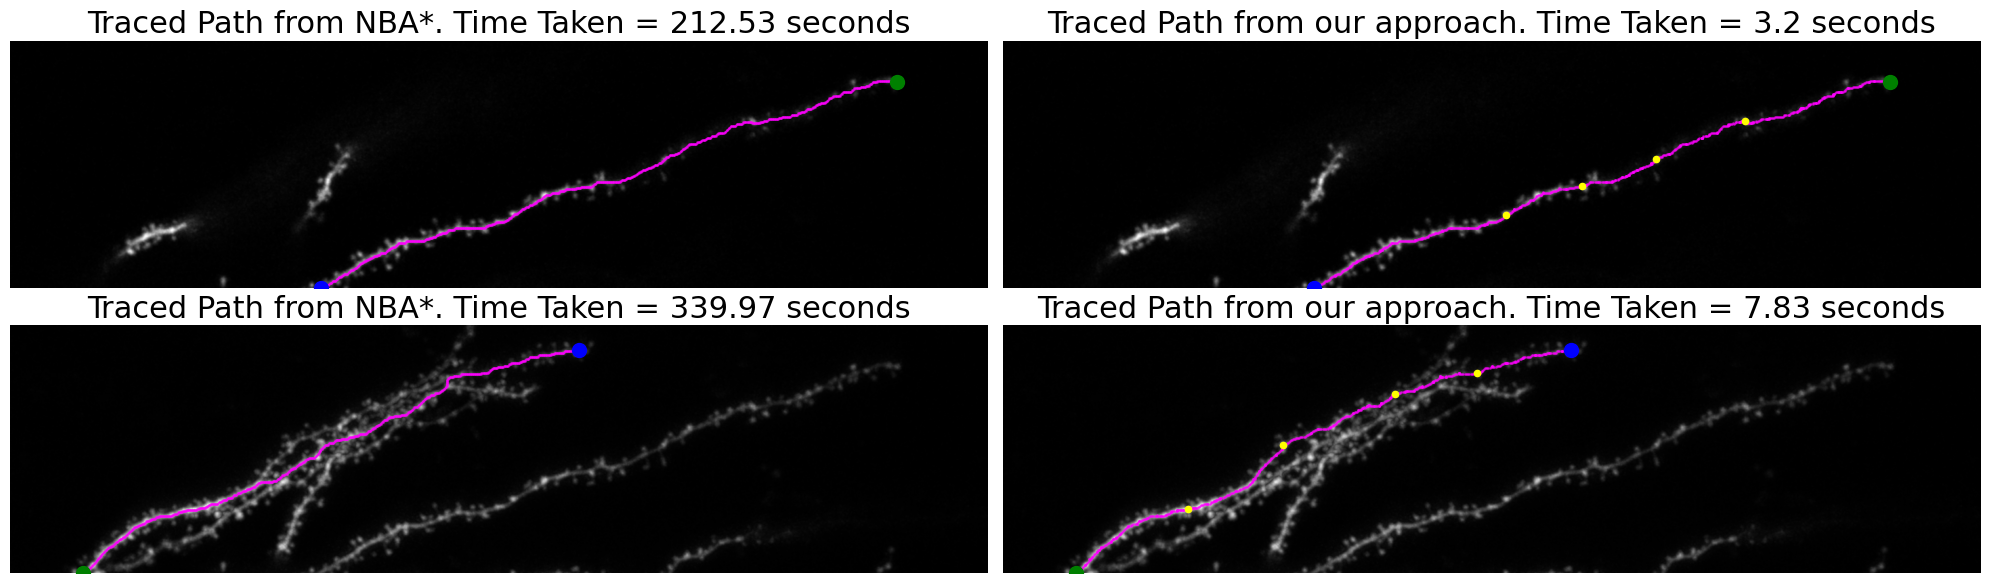
\includegraphics[width=0.95\textwidth]{figures/32_path_comparison.png}
\captionof{figure}{Comparison of dendrite path tracing: NBA* vs Neuro-\gls{SAM}. Traces generated using the original brightest-path-lib (left) and our modified waypoint-aware module (right). Scale: $0.94\,\mu\text{m}/\text{px}$}
\label{fig:path_comparison}
\end{center}

\subsection{Segmentation Module}

Following path tracing, the segmentation module in Neuro-\gls{SAM} performs segmentation of dendrite shafts using a refined adaptation of \gls{SAMv2}. Unlike earlier models that relied on generic grid prompts or local feature points, our pipeline leverages the traced dendrite path to sample overlapping patches and extract precise, geometry-aware prompts. This path-conditioned prompting strategy allows Neuro-\gls{SAM} to generate spatially coherent segmentations even in regions with low contrast, occlusions, or complex curvature. The segmentation model was trained on high-resolution volumes with custom prompt tuning and inference postprocessing, ensuring robustness across multiple datasets.

\begin{center}
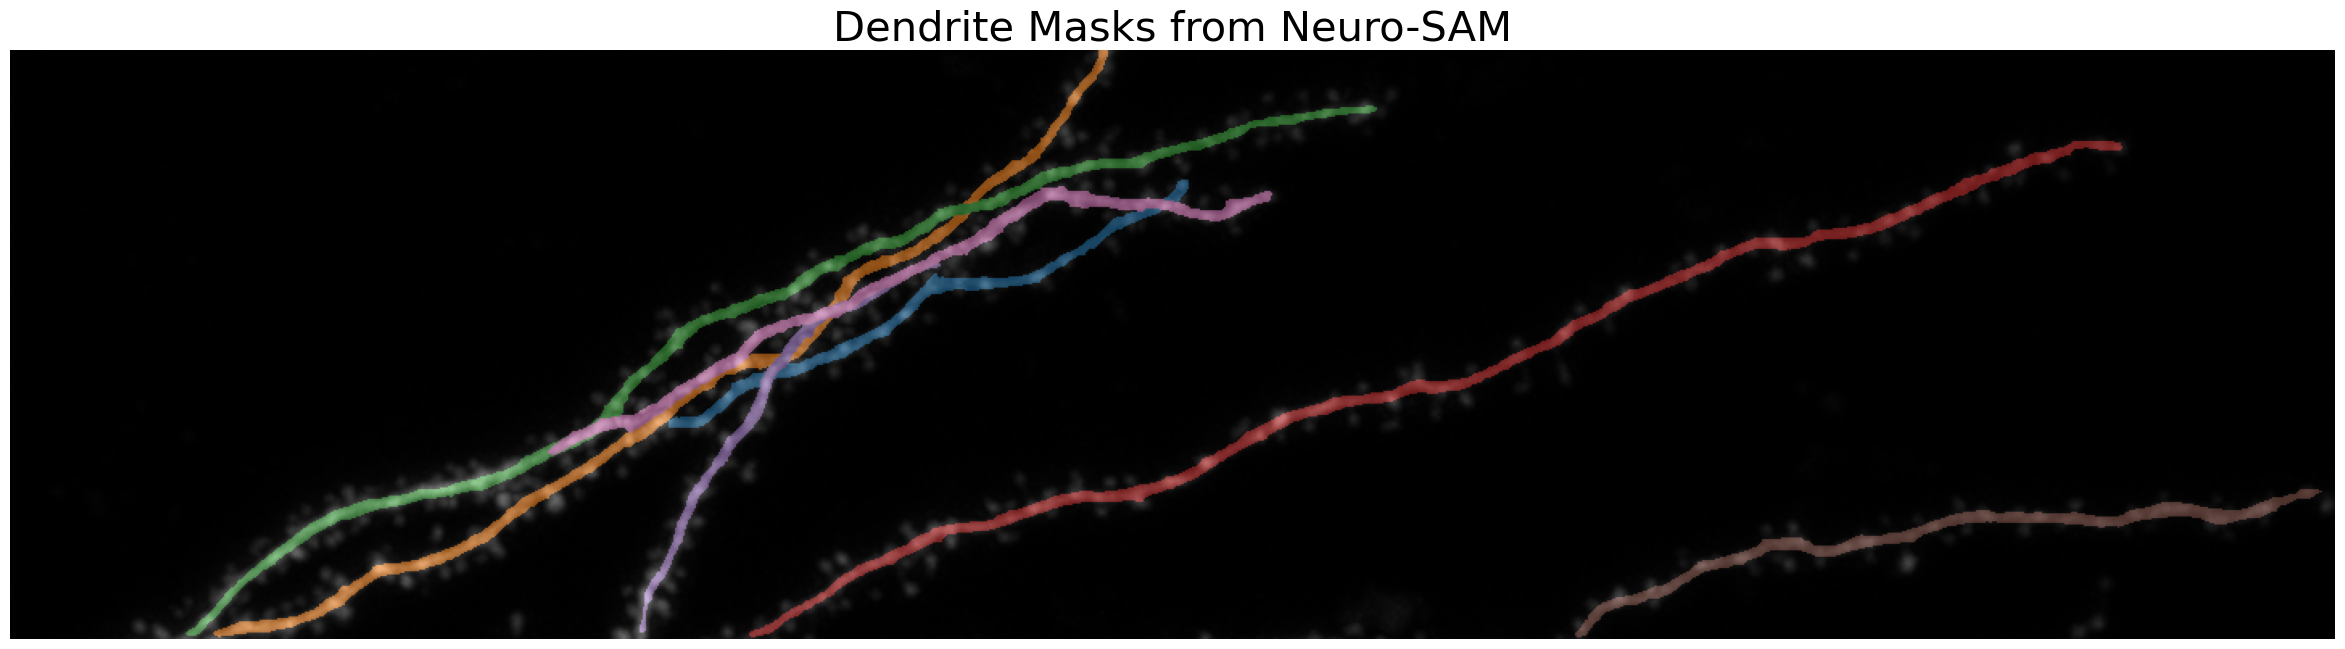
\includegraphics[width=0.95\textwidth]{figures/33_dendrite_seg_all.png}
\captionof{figure}{Predicted dendrite masks from Neuro-\gls{SAM} overlaid on the benchmark stack. Each dendritic shaft is segmented individually and visualized in different colours. Scale: $0.94\,\mu\text{m}/\text{px}$}
\label{fig:dendrite_seg_all}
\end{center}

The segmentation results from Neuro-\gls{SAM} exhibit highly accurate dendritic masks, closely following the underlying morphology traced in the benchmark image stack. As shown in \autoref{fig:dendrite_seg_all}, each dendrite is individually segmented and rendered with clear boundaries, even in curved regions and near other dendrites. The ability to isolate individual shafts across the 3D stack ( \autoref{fig:separate_masks}) further confirms the spatial coherence and continuity achieved by our path-conditioned prompting strategy.

\begin{center}
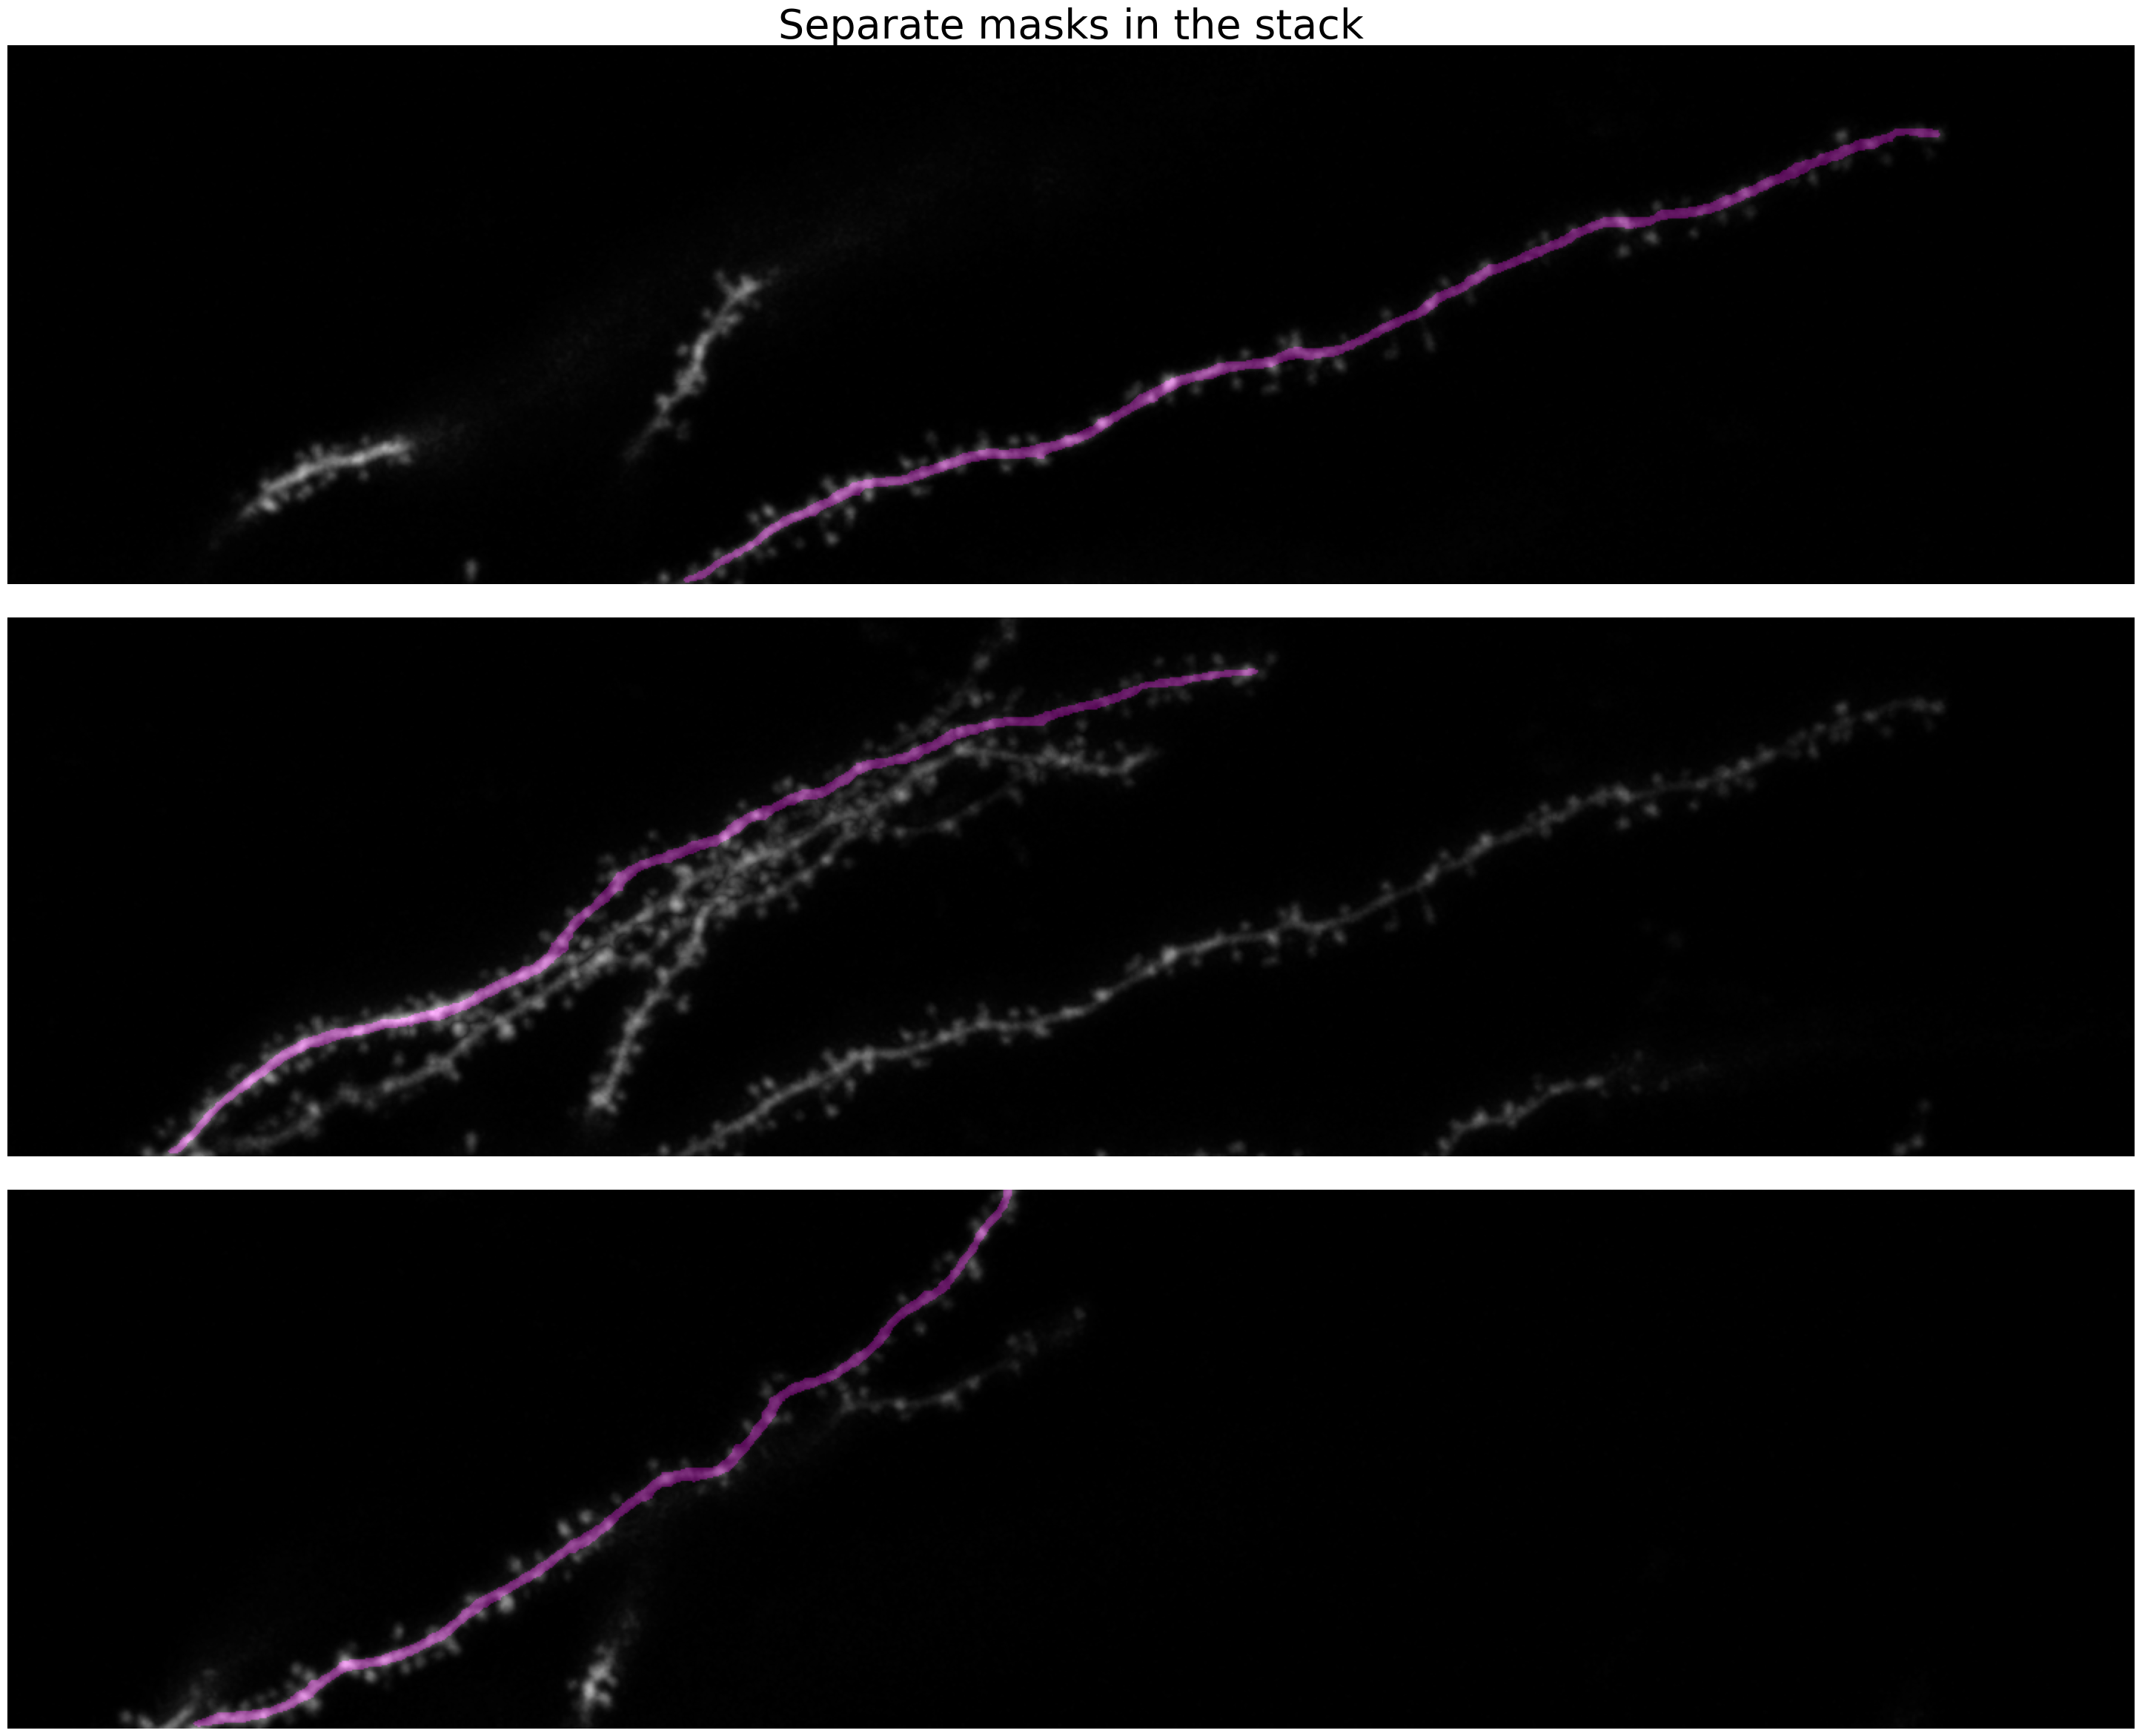
\includegraphics[width=0.9\textwidth]{figures/34_separate_masks.png}
\captionof{figure}{Individual dendrite segmentations from Neuro-\gls{SAM} shown across different regions of the stack. Scale: $0.94\,\mu\text{m}/\text{px}$}
\label{fig:separate_masks}
\end{center}

\begin{center}
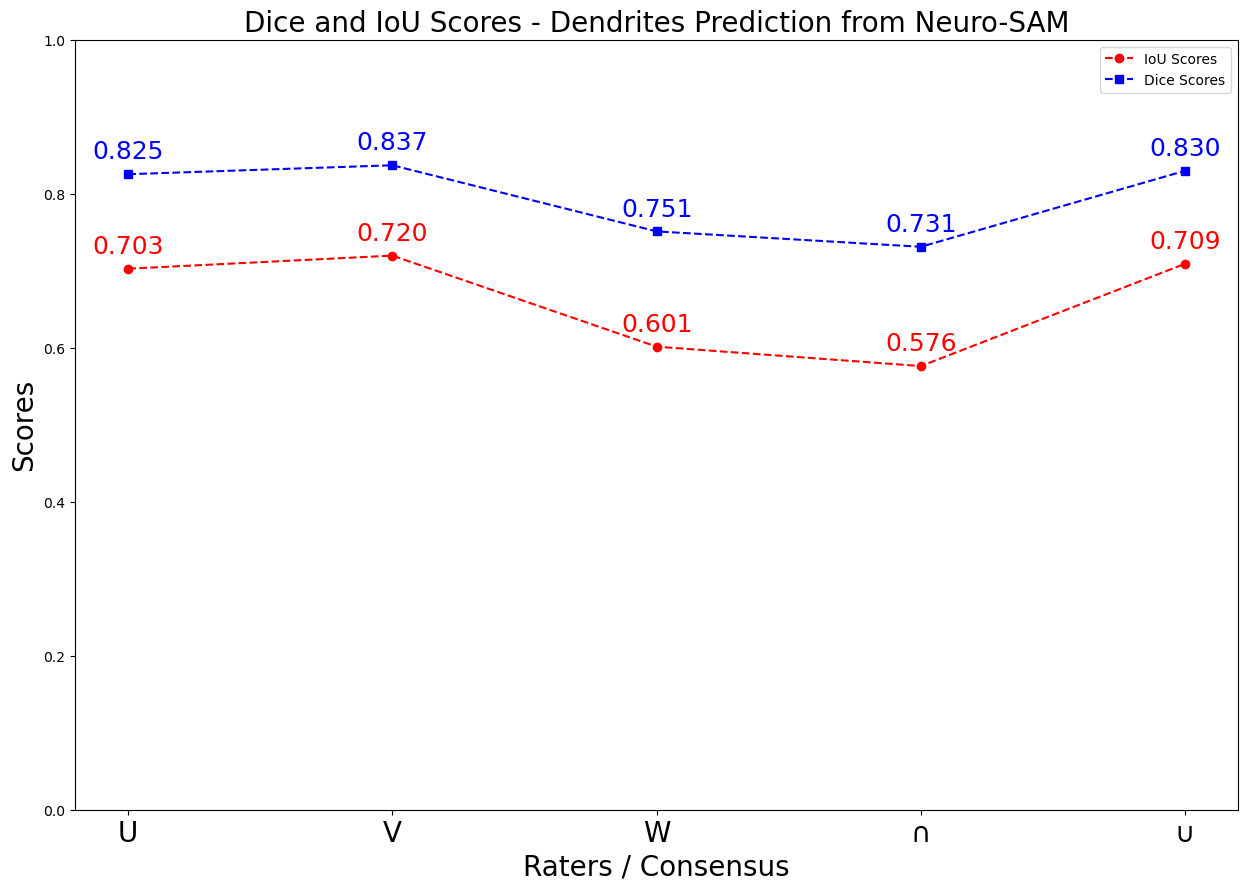
\includegraphics[width=0.7\textwidth]{figures/35_dendrite_metric_neurosam.png}
\captionof{figure}{Dice and \gls{IoU} scores for dendrite predictions from Neuro-\gls{SAM} across different raters and consensus masks.}
\label{fig:dendrite_metric_neurosam}
\end{center}

As visualized in \autoref{fig:dendrite_metric_neurosam}, Neuro-\gls{SAM} achieves consistently high Dice and \gls{IoU} scores across all raters and consensus annotations, with Dice values reaching up to 0.837 and \gls{IoU} up to 0.720. These numbers significantly outperform prior variants, including base \gls{SAM}, \gls{SAM}+\gls{LoRA} and \gls{DeepD3}, demonstrating the effectiveness of our prompt tuning and training strategy. The low variance across raters also indicates stable generalization across inter-rater variability and imaging conditions.



\begin{center}
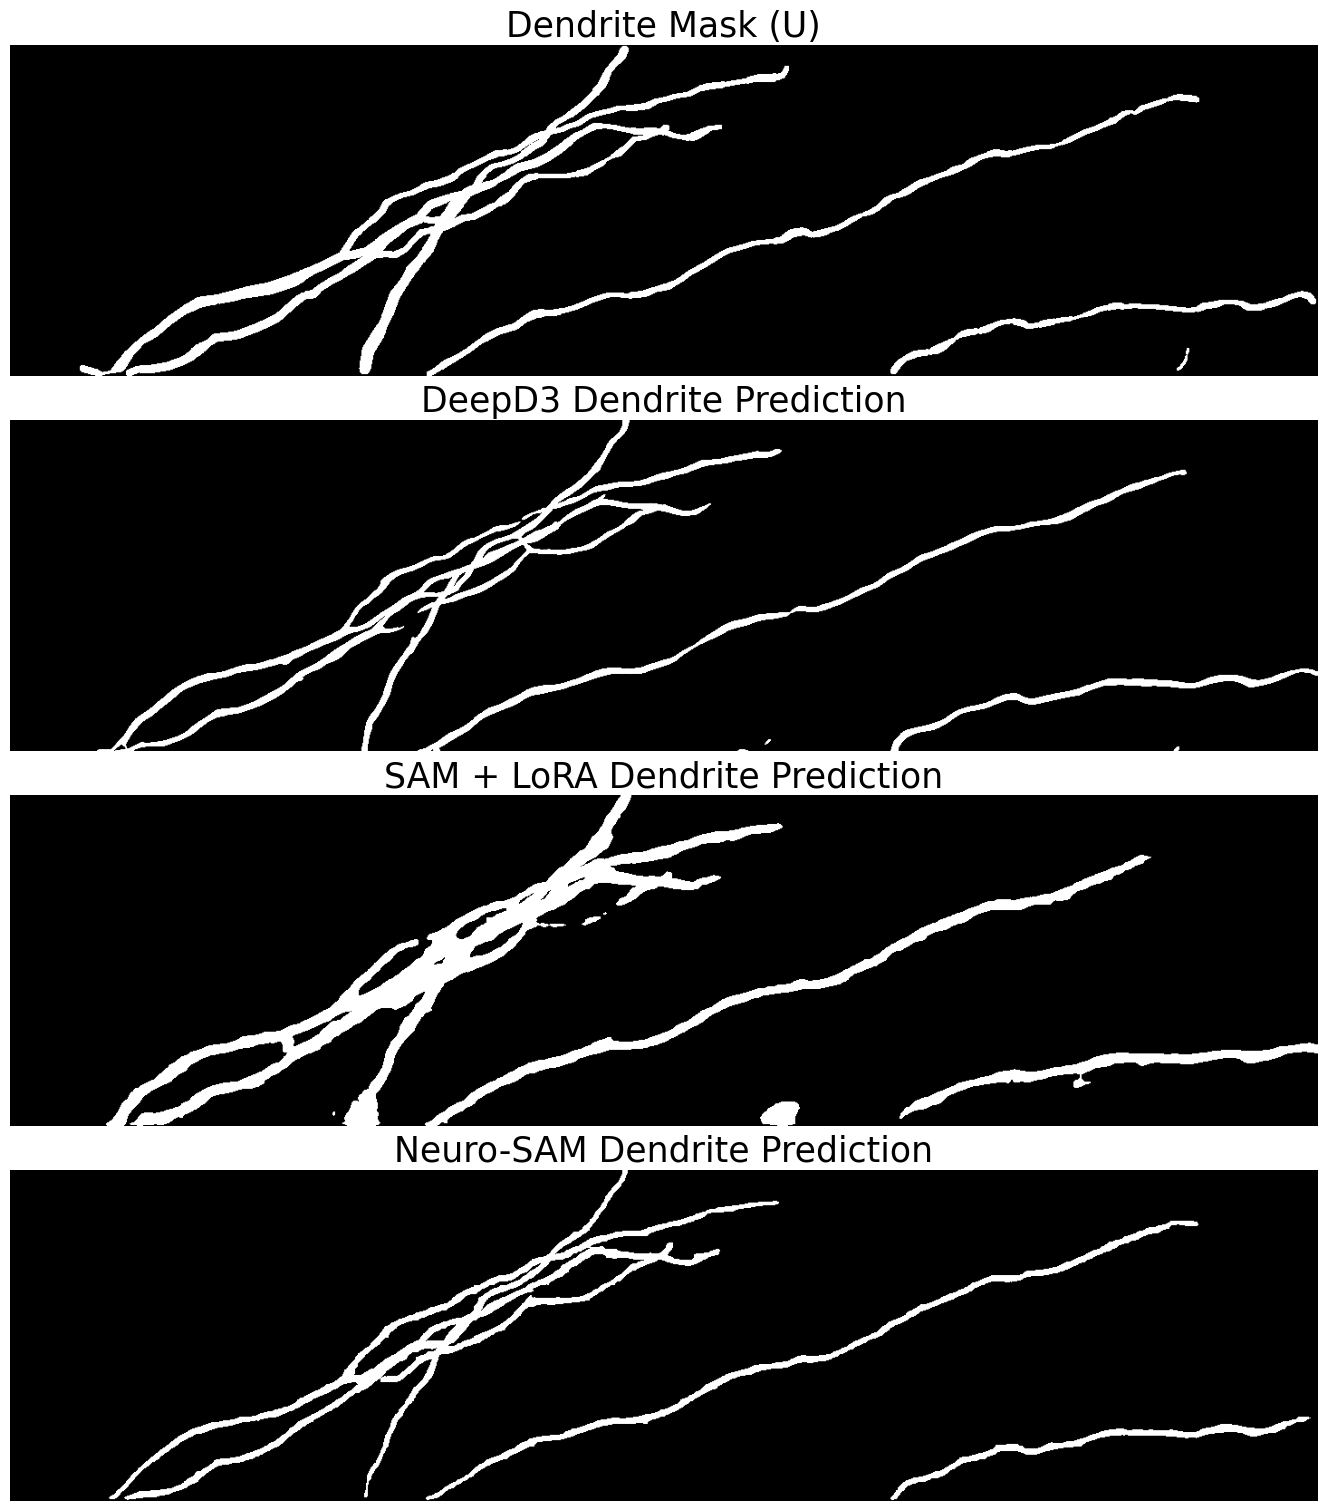
\includegraphics[width=0.65\textwidth]{figures/36_dendrite_compare_mask.png}
\captionof{figure}{Qualitative comparison of dendrite predictions from \gls{DeepD3}, \gls{SAM}+\gls{LoRA}, and Neuro-\gls{SAM} against the rater U mask. Neuro-\gls{SAM} demonstrates improved completeness and accuracy of segmentation, particularly in overlapping dendrites. Scale: $0.94\,\mu\text{m}/\text{px}$}
\label{fig:dendrite_compare_mask}
\end{center}

The comparative plot in \autoref{fig:dendrite_compare_mask} highlights the improvement of Neuro-\gls{SAM} over \gls{DeepD3} and \gls{SAM}+\gls{LoRA}. While \gls{DeepD3} captures overall structure, it often exhibits disconnected segments and under-segmentation in thinner regions. \gls{SAM}+\gls{LoRA}, though denser, tends to over-segment and merge adjacent shafts. In contrast, Neuro-\gls{SAM} provides precise, well-delimited masks that remain faithful to the ground truth. This is further reinforced in per-frame comparisons (\autoref{fig:compare_frame_masks}), where Neuro-\gls{SAM} reliably segments long dendritic stretches with better spatial continuity and fewer artifacts. It not only segments the dendrites better but with the help of Path Tracing algorithm, it even traces the dendrite regions that are often lacking in the masks but visible to the human eye. 

\begin{center}
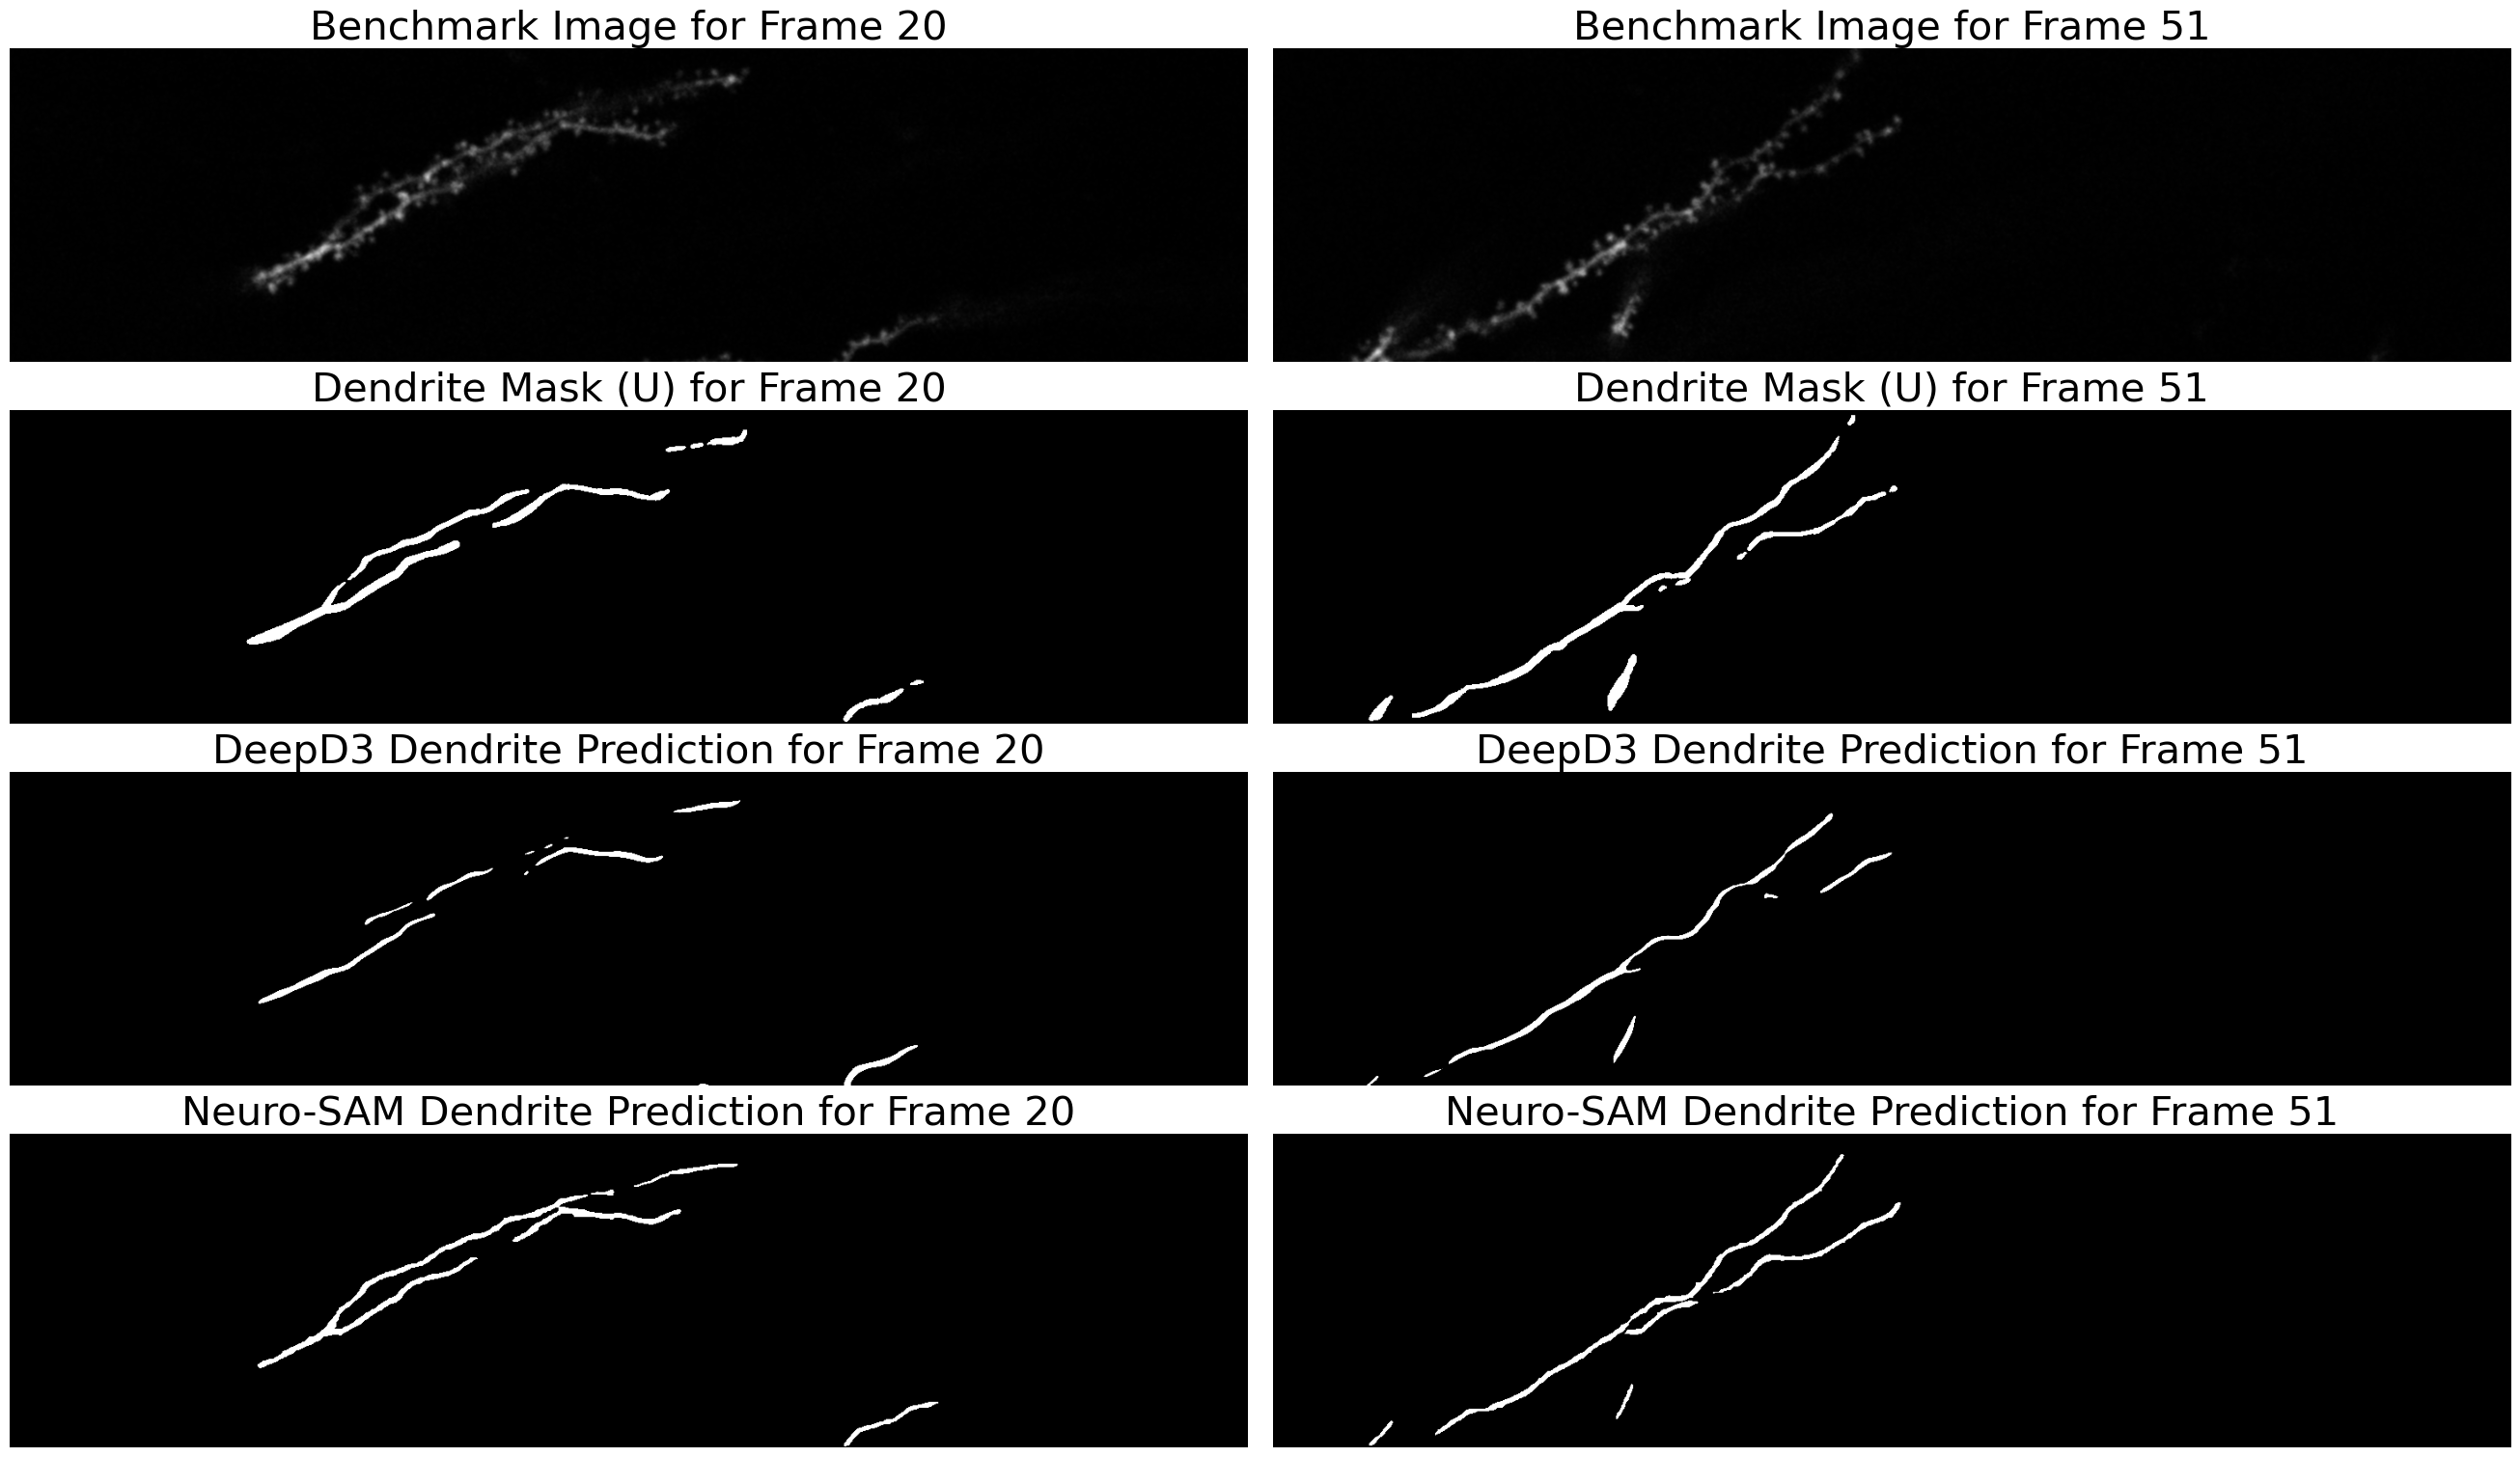
\includegraphics[width=0.95\textwidth]{figures/37_compare_frame_masks.png}
\captionof{figure}{Frame-wise comparison of dendrite predictions on benchmark images at timepoints 20 and 51. Neuro-\gls{SAM} consistently provides more complete and precise segmentations compared to \gls{DeepD3}, with better adherence to ground truth masks. Scale: $0.94\,\mu\text{m}/\text{px}$}
\label{fig:compare_frame_masks}
\end{center}

To contextualize performance, we compared Neuro-\gls{SAM} against \gls{DeepD3} across all raters and consensus masks. As shown in \autoref{fig:dendrite_metrics_comparison}, Neuro-\gls{SAM} consistently achieves slightly higher Dice and \gls{IoU} scores across all evaluations. These gains can be attributed to its geometry-aware prompting and tight integration with the traced path, which enhances mask continuity and alignment with dendritic morphology. In contrast, \gls{DeepD3} exhibits good performance but shows occasional fragmentation or missed segments, particularly in low-contrast or overlapping regions.

\begin{center}
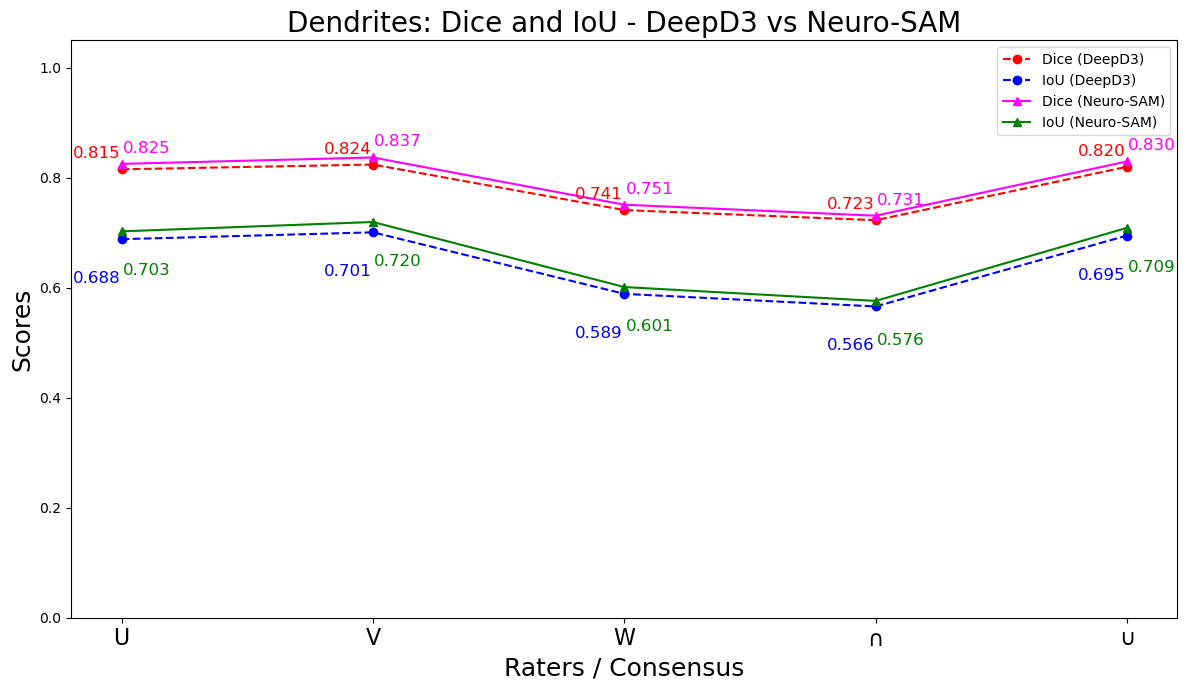
\includegraphics[width=0.9\textwidth]{figures/45_dendrite_metrics_comparison.png}
\captionof{figure}{Quantitative comparison of dendrite segmentation performance between \gls{DeepD3} and Neuro-\gls{SAM}. Neuro-\gls{SAM} consistently outperforms \gls{DeepD3} across all raters and consensus masks in both Dice and \gls{IoU} metrics.}
\label{fig:dendrite_metrics_comparison}
\end{center}



Overall, these results validate the efficacy of Neuro-\gls{SAM}'s path-aware segmentation mechanism. By leveraging path geometry as a guiding prior, our model not only improves accuracy but also enables robust, high-fidelity segmentation of dendrites at scale. This makes Neuro-\gls{SAM} a strong candidate for integration into large-scale dendrite quantification, especially in datasets with high structural complexity and minimal annotations.

\subsection{Spine Segmentation Module}
The final stage of Neuro-\gls{SAM} involves the segmentation of individual dendritic spines, which represent the most granular structures in the neural imaging pipeline. Building upon the traced dendrite shafts and their corresponding segmentations, spine segmentation is performed in a spatially localized and context-aware manner. Each spine is identified along the predicted shaft, allowing the model to isolate small, closely packed protrusions without relying on pixel-wise annotations. This section presents both qualitative and quantitative results of Neuro-\gls{SAM}'s spine segmentation performance, benchmarked against expert annotations and compared with \gls{DeepD3} predictions.

\begin{center}
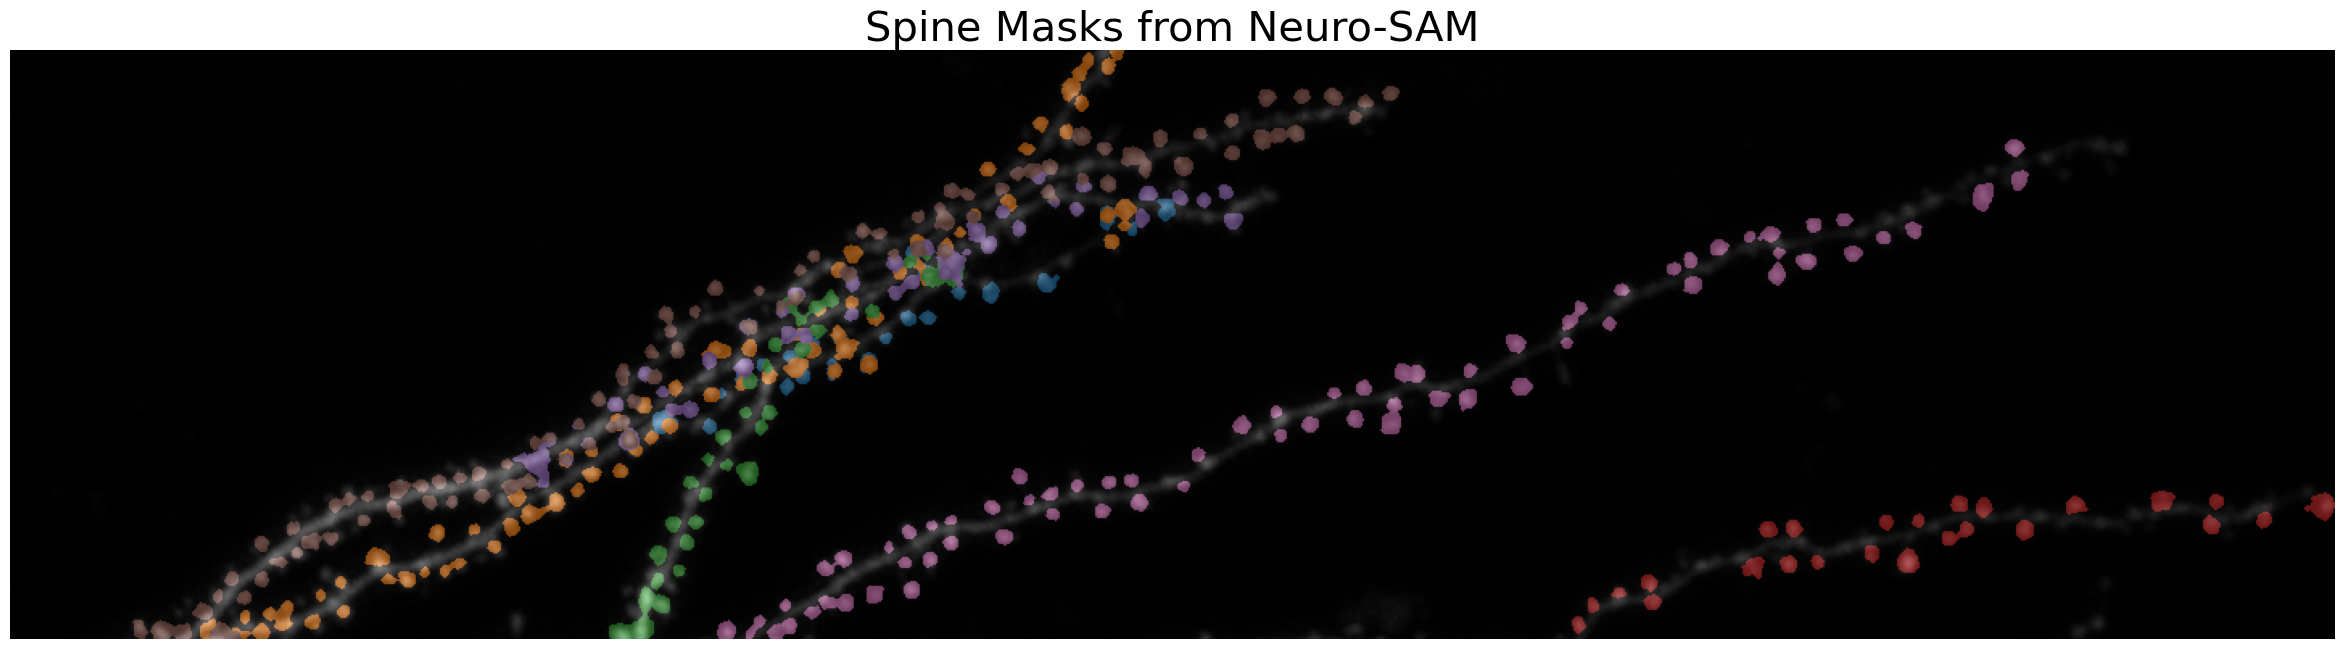
\includegraphics[width=0.95\textwidth]{figures/38_spine_seg_all.png}
\captionof{figure}{Overlay of spine segmentation masks predicted by Neuro-\gls{SAM} on the benchmark volume. Each spine instance is shown in a distinct color. The model localizes individual spines along dendritic shafts across diverse morphologies and densities. Scale: $0.94\,\mu\text{m}/\text{px}$}
\label{fig:spine_seg_all}
\end{center}

A representative visualization of spine segmentation masks generated by Neuro-\gls{SAM} is shown in \autoref{fig:spine_seg_all}, overlaid on the original benchmark stack. The output exhibits well-localized, evenly distributed spine predictions along the dendritic paths, capturing a wide range of spine shapes and sizes. To better illustrate prediction consistency, \autoref{fig:separate_spine_masks} presents slice-wise overlays of segmented spines on three traced paths from the volume. The predicted masks align closely with ground-truth spines, even in regions with densely clustered structures and low image contrast.

\begin{center}
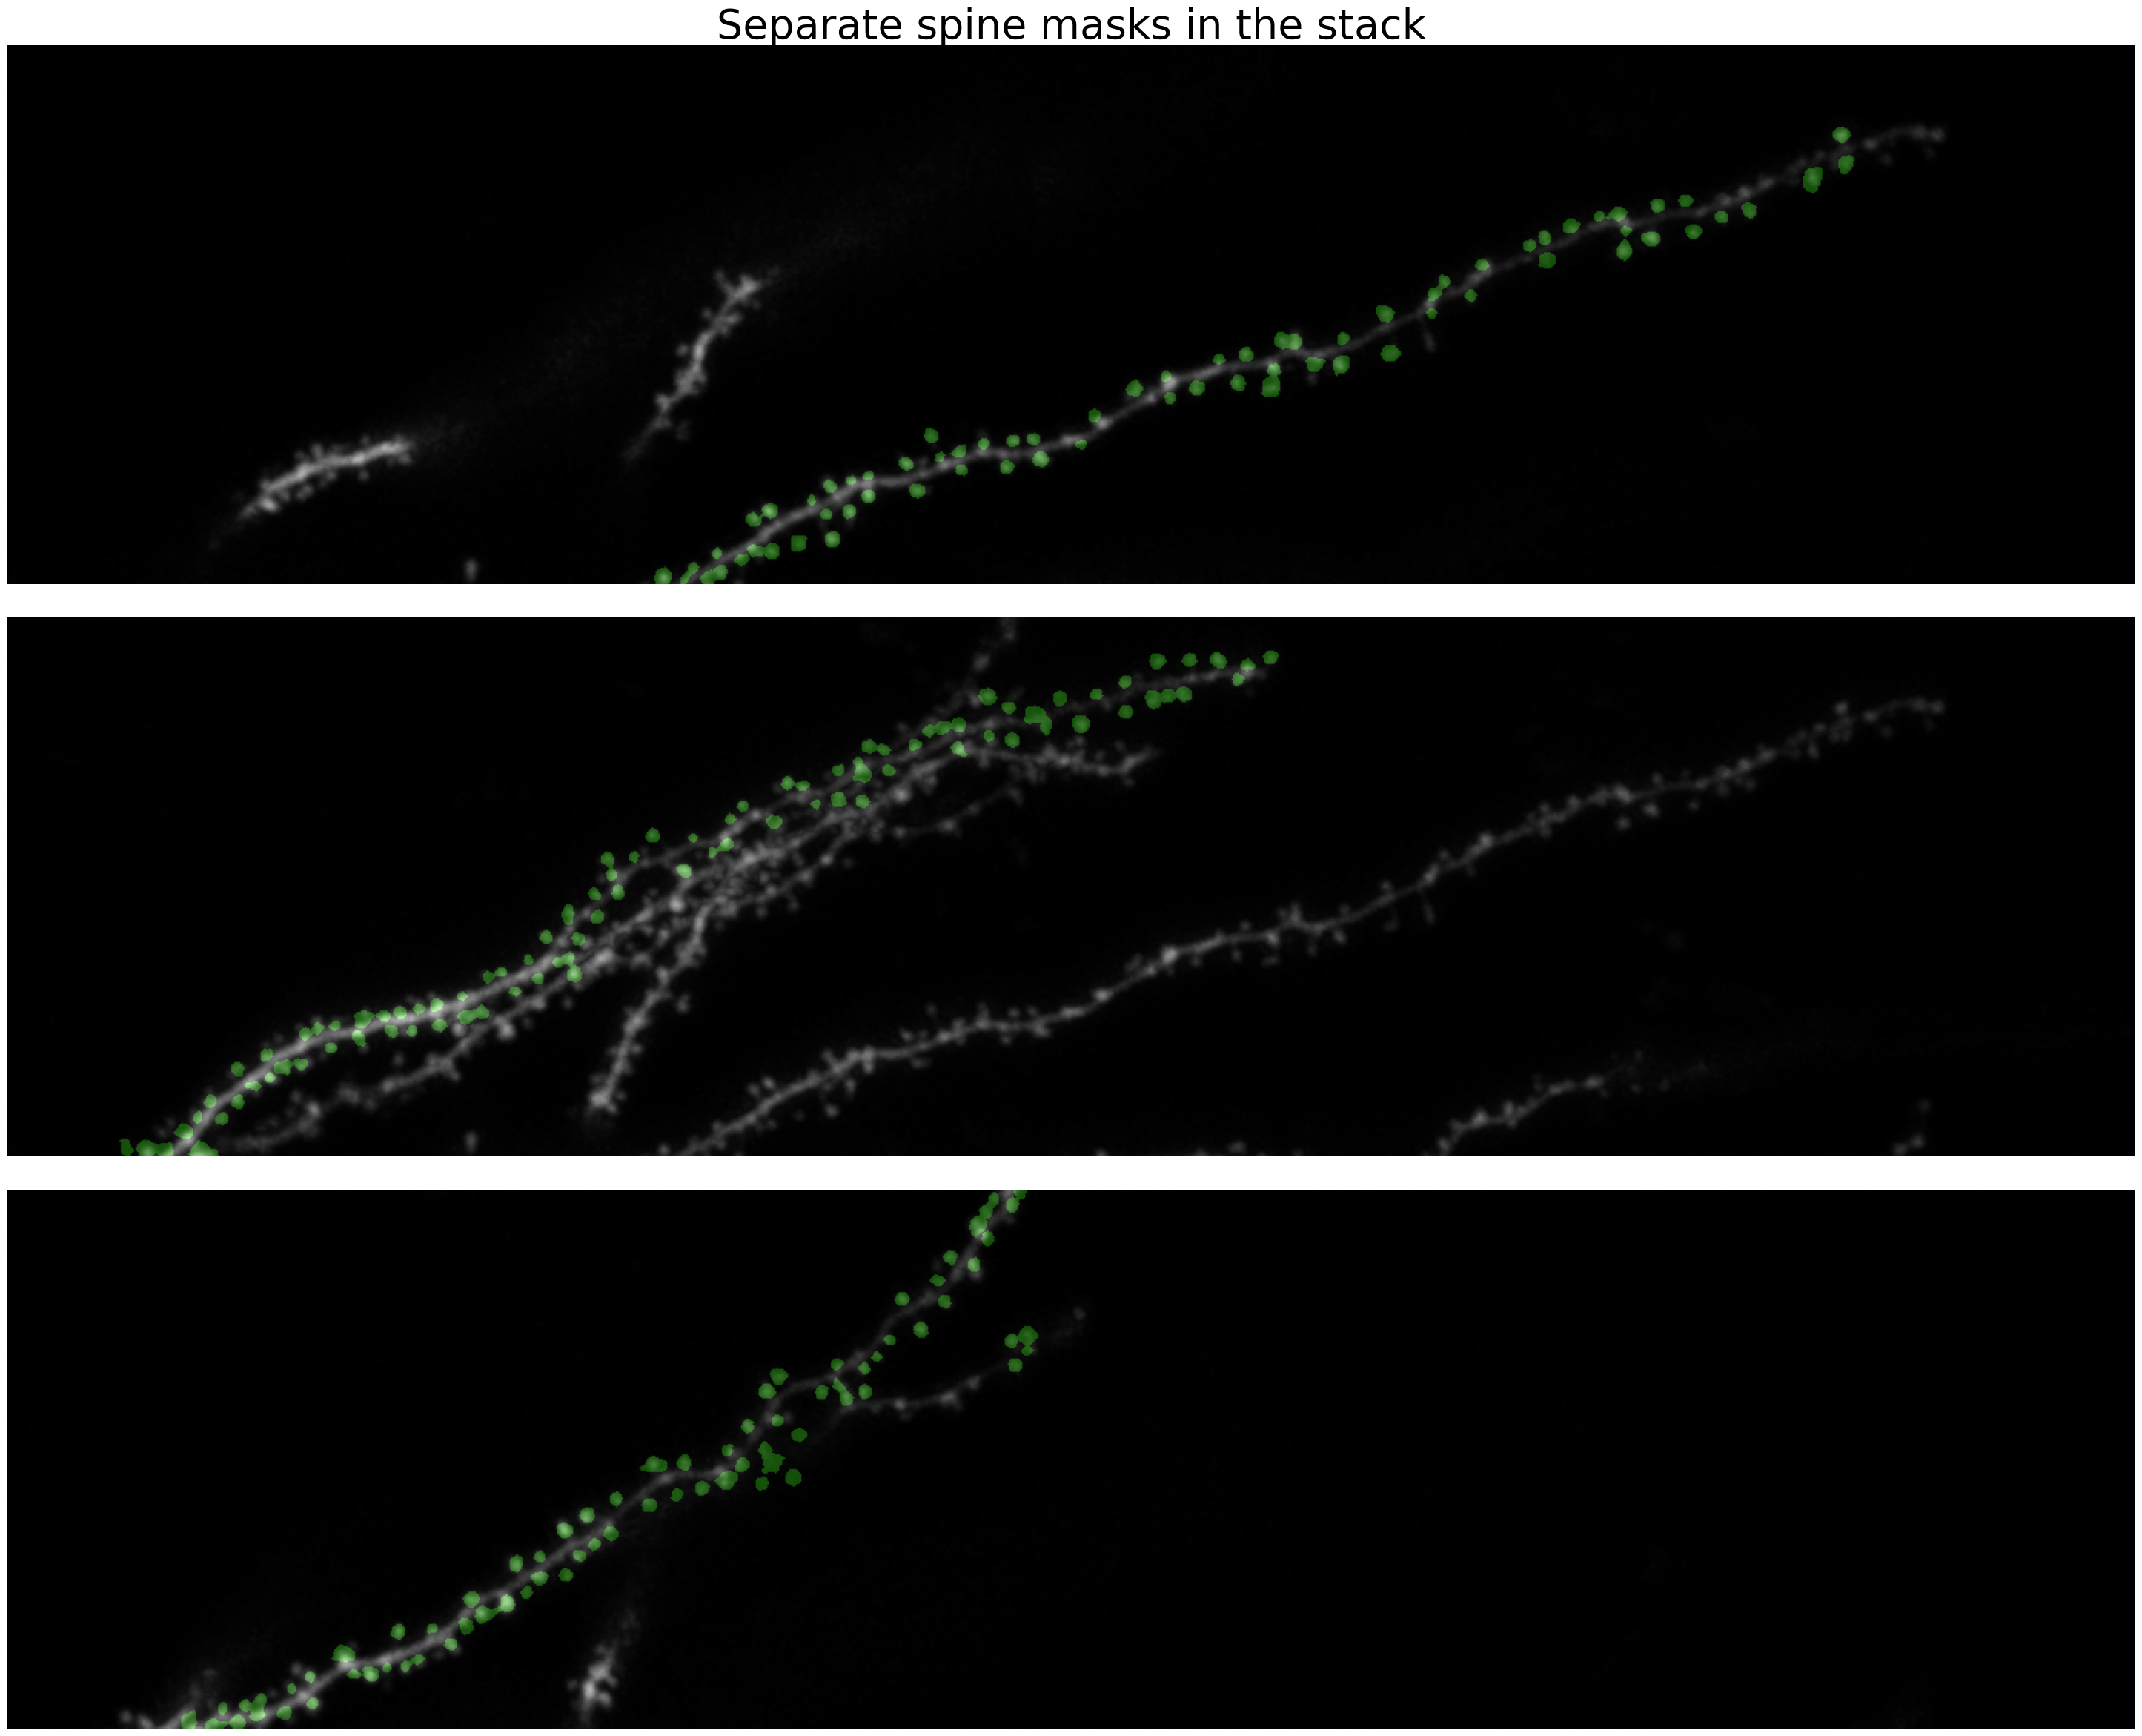
\includegraphics[width=0.8\textwidth]{figures/39_compare_frame_masks.png}
\captionof{figure}{Slice-wise visualization of predicted spines (green) by Neuro-\gls{SAM} on traced dendrites from the benchmark stack. Despite high spine density and low contrast regions, the model maintains spatial accuracy and continuity. Scale: $0.94\,\mu\text{m}/\text{px}$}
\label{fig:separate_spine_masks}
\end{center}

\begin{center}
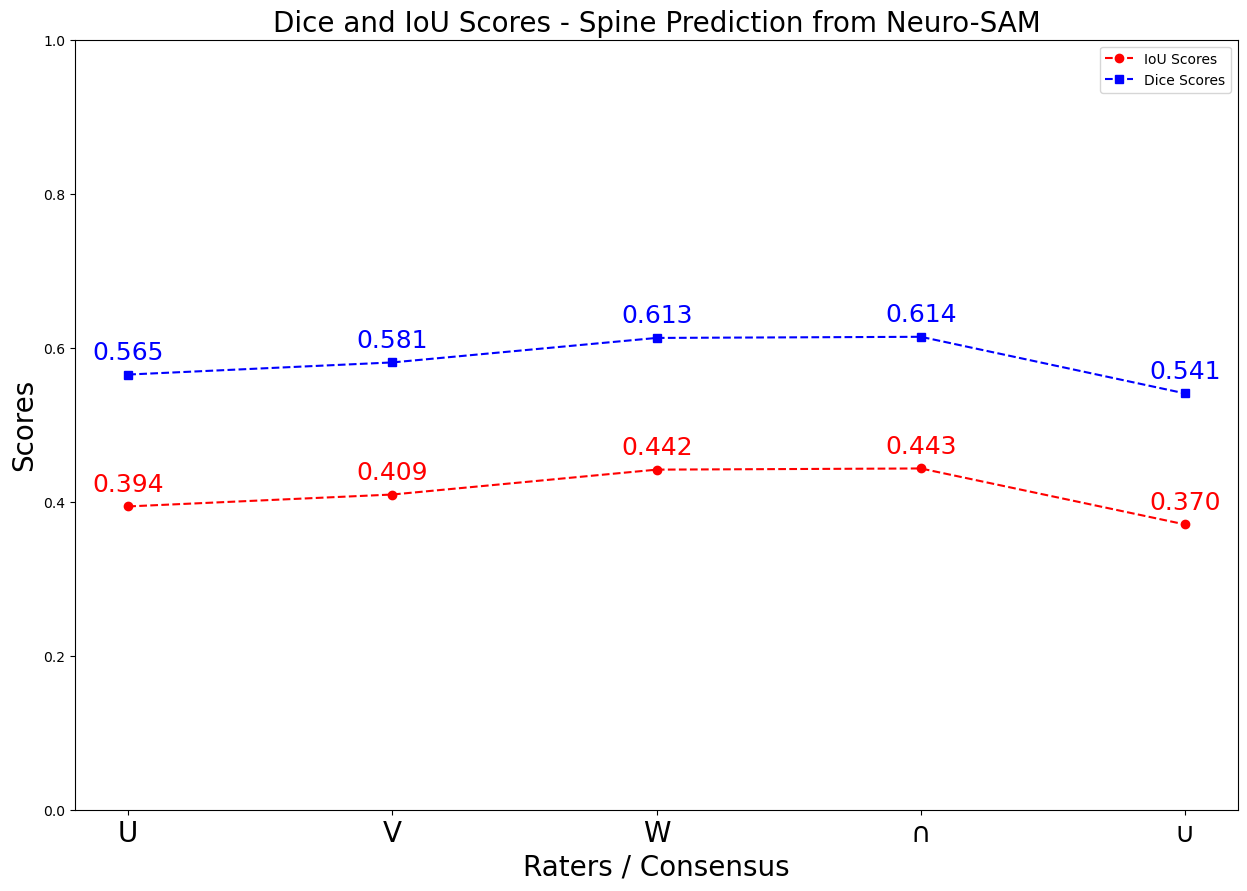
\includegraphics[width=0.8\textwidth]{figures/40_spine_seg_metrics.png}
\captionof{figure}{Quantitative evaluation of spine segmentation performance. Dice and \gls{IoU} scores from Neuro-\gls{SAM} predictions are computed against annotations from three human raters and the consensus. The model demonstrates consistent performance with minimal variability across raters.}
\label{fig:spine_seg_metrics}
\end{center}

Quantitative evaluation of spine segmentation performance is summarized in \autoref{fig:spine_seg_metrics}. Dice and \gls{IoU} scores across three raters and the unified consensus annotation highlight a strong performance by Neuro-\gls{SAM}, with average Dice scores ranging from 0.54 to 0.61 across raters. While performance is generally lower than dendrite segmentation due to the complexity and small size of spines, the consistency across raters indicates reliable model behavior.

\autoref{fig:spine_seg_comparison} compares spine segmentation outputs from \gls{DeepD3} and Neuro-\gls{SAM} against rater U. \gls{DeepD3} often shows slight over-segmentation and fragmented spines, whereas Neuro-\gls{SAM} yields more spatially compact and discrete spine masks. Finally, \autoref{fig:spine_seg_per_frame} shows per-frame performance comparisons, highlighting Neuro-\gls{SAM}’s capacity to maintain segmentation quality across diverse spatial regions and imaging conditions.


\begin{center}
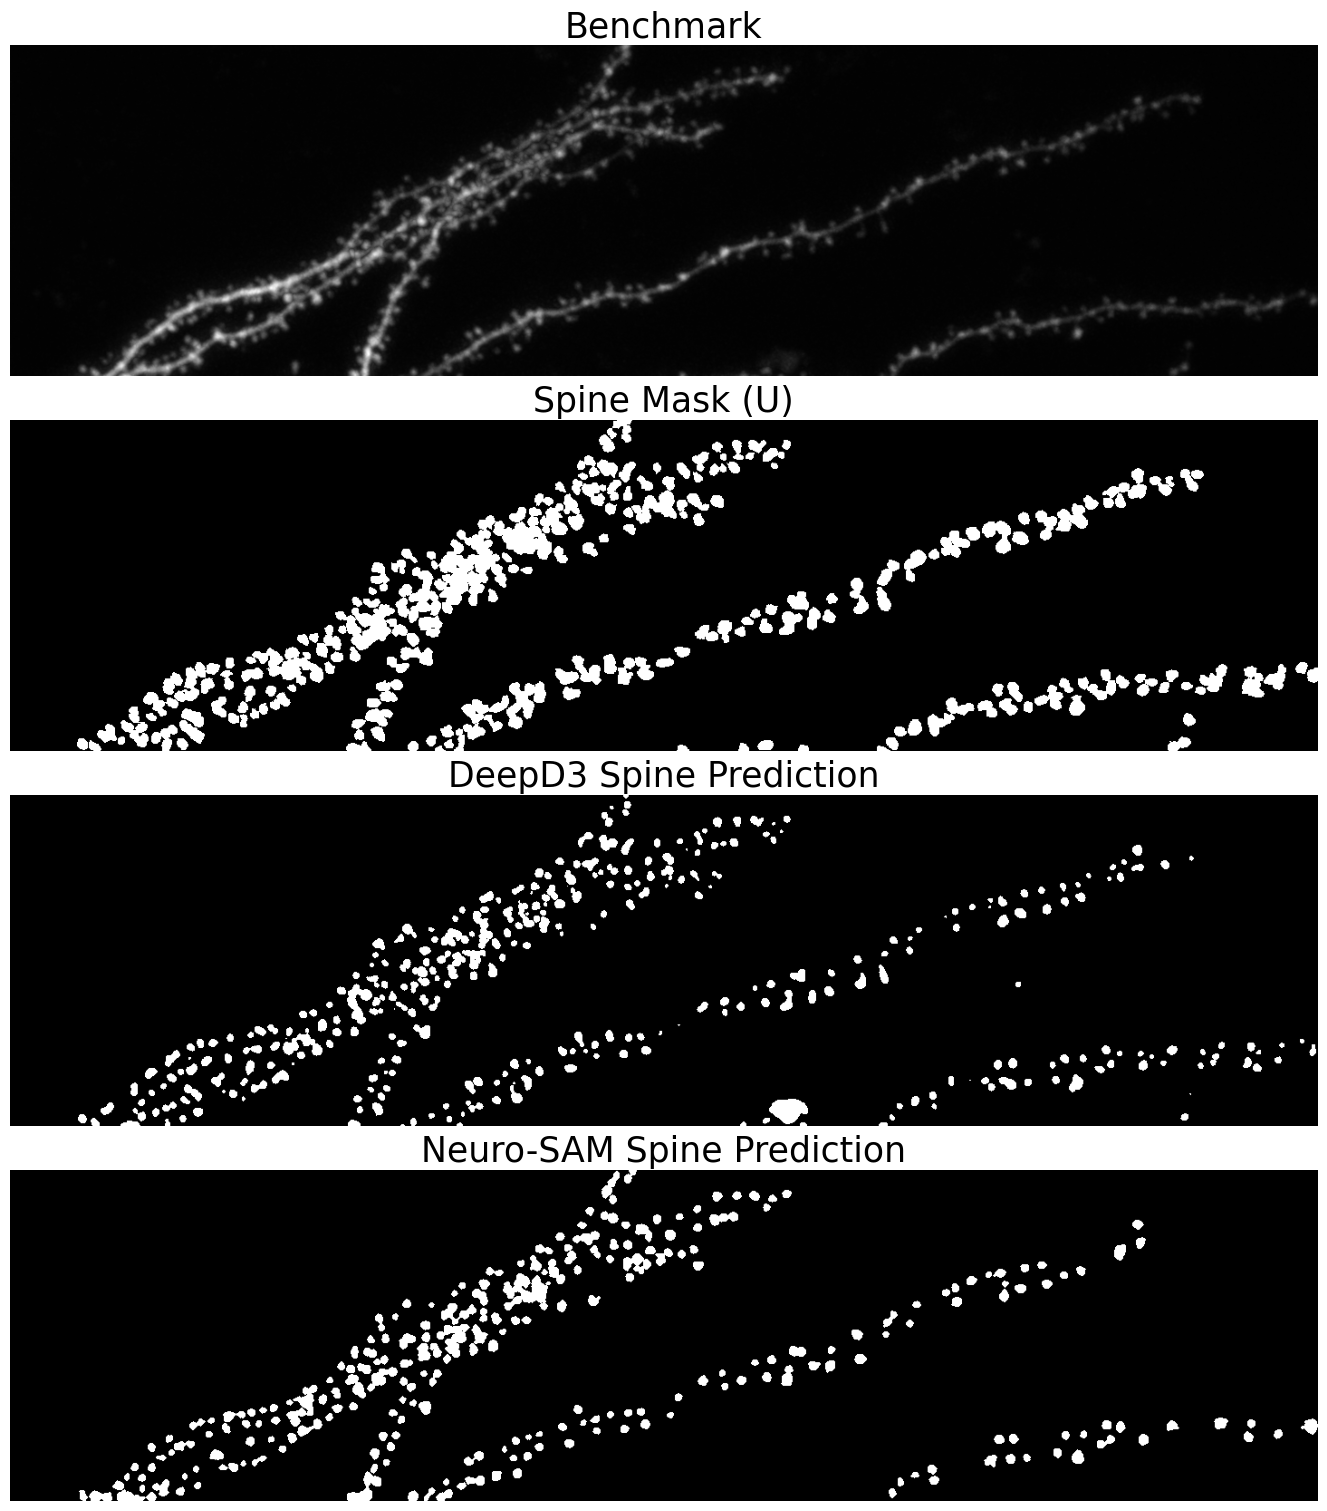
\includegraphics[width=0.9\textwidth]{figures/41_spine_seg_comparison.png}
\captionof{figure}{Comparative analysis of spine segmentation predictions from \gls{DeepD3} and Neuro-\gls{SAM}, with ground truth from rater U. Neuro-\gls{SAM} outputs exhibit better shape compactness and fewer false positives than \gls{DeepD3}. Scale: $0.94\,\mu\text{m}/\text{px}$}
\label{fig:spine_seg_comparison}
\end{center}


\begin{center}
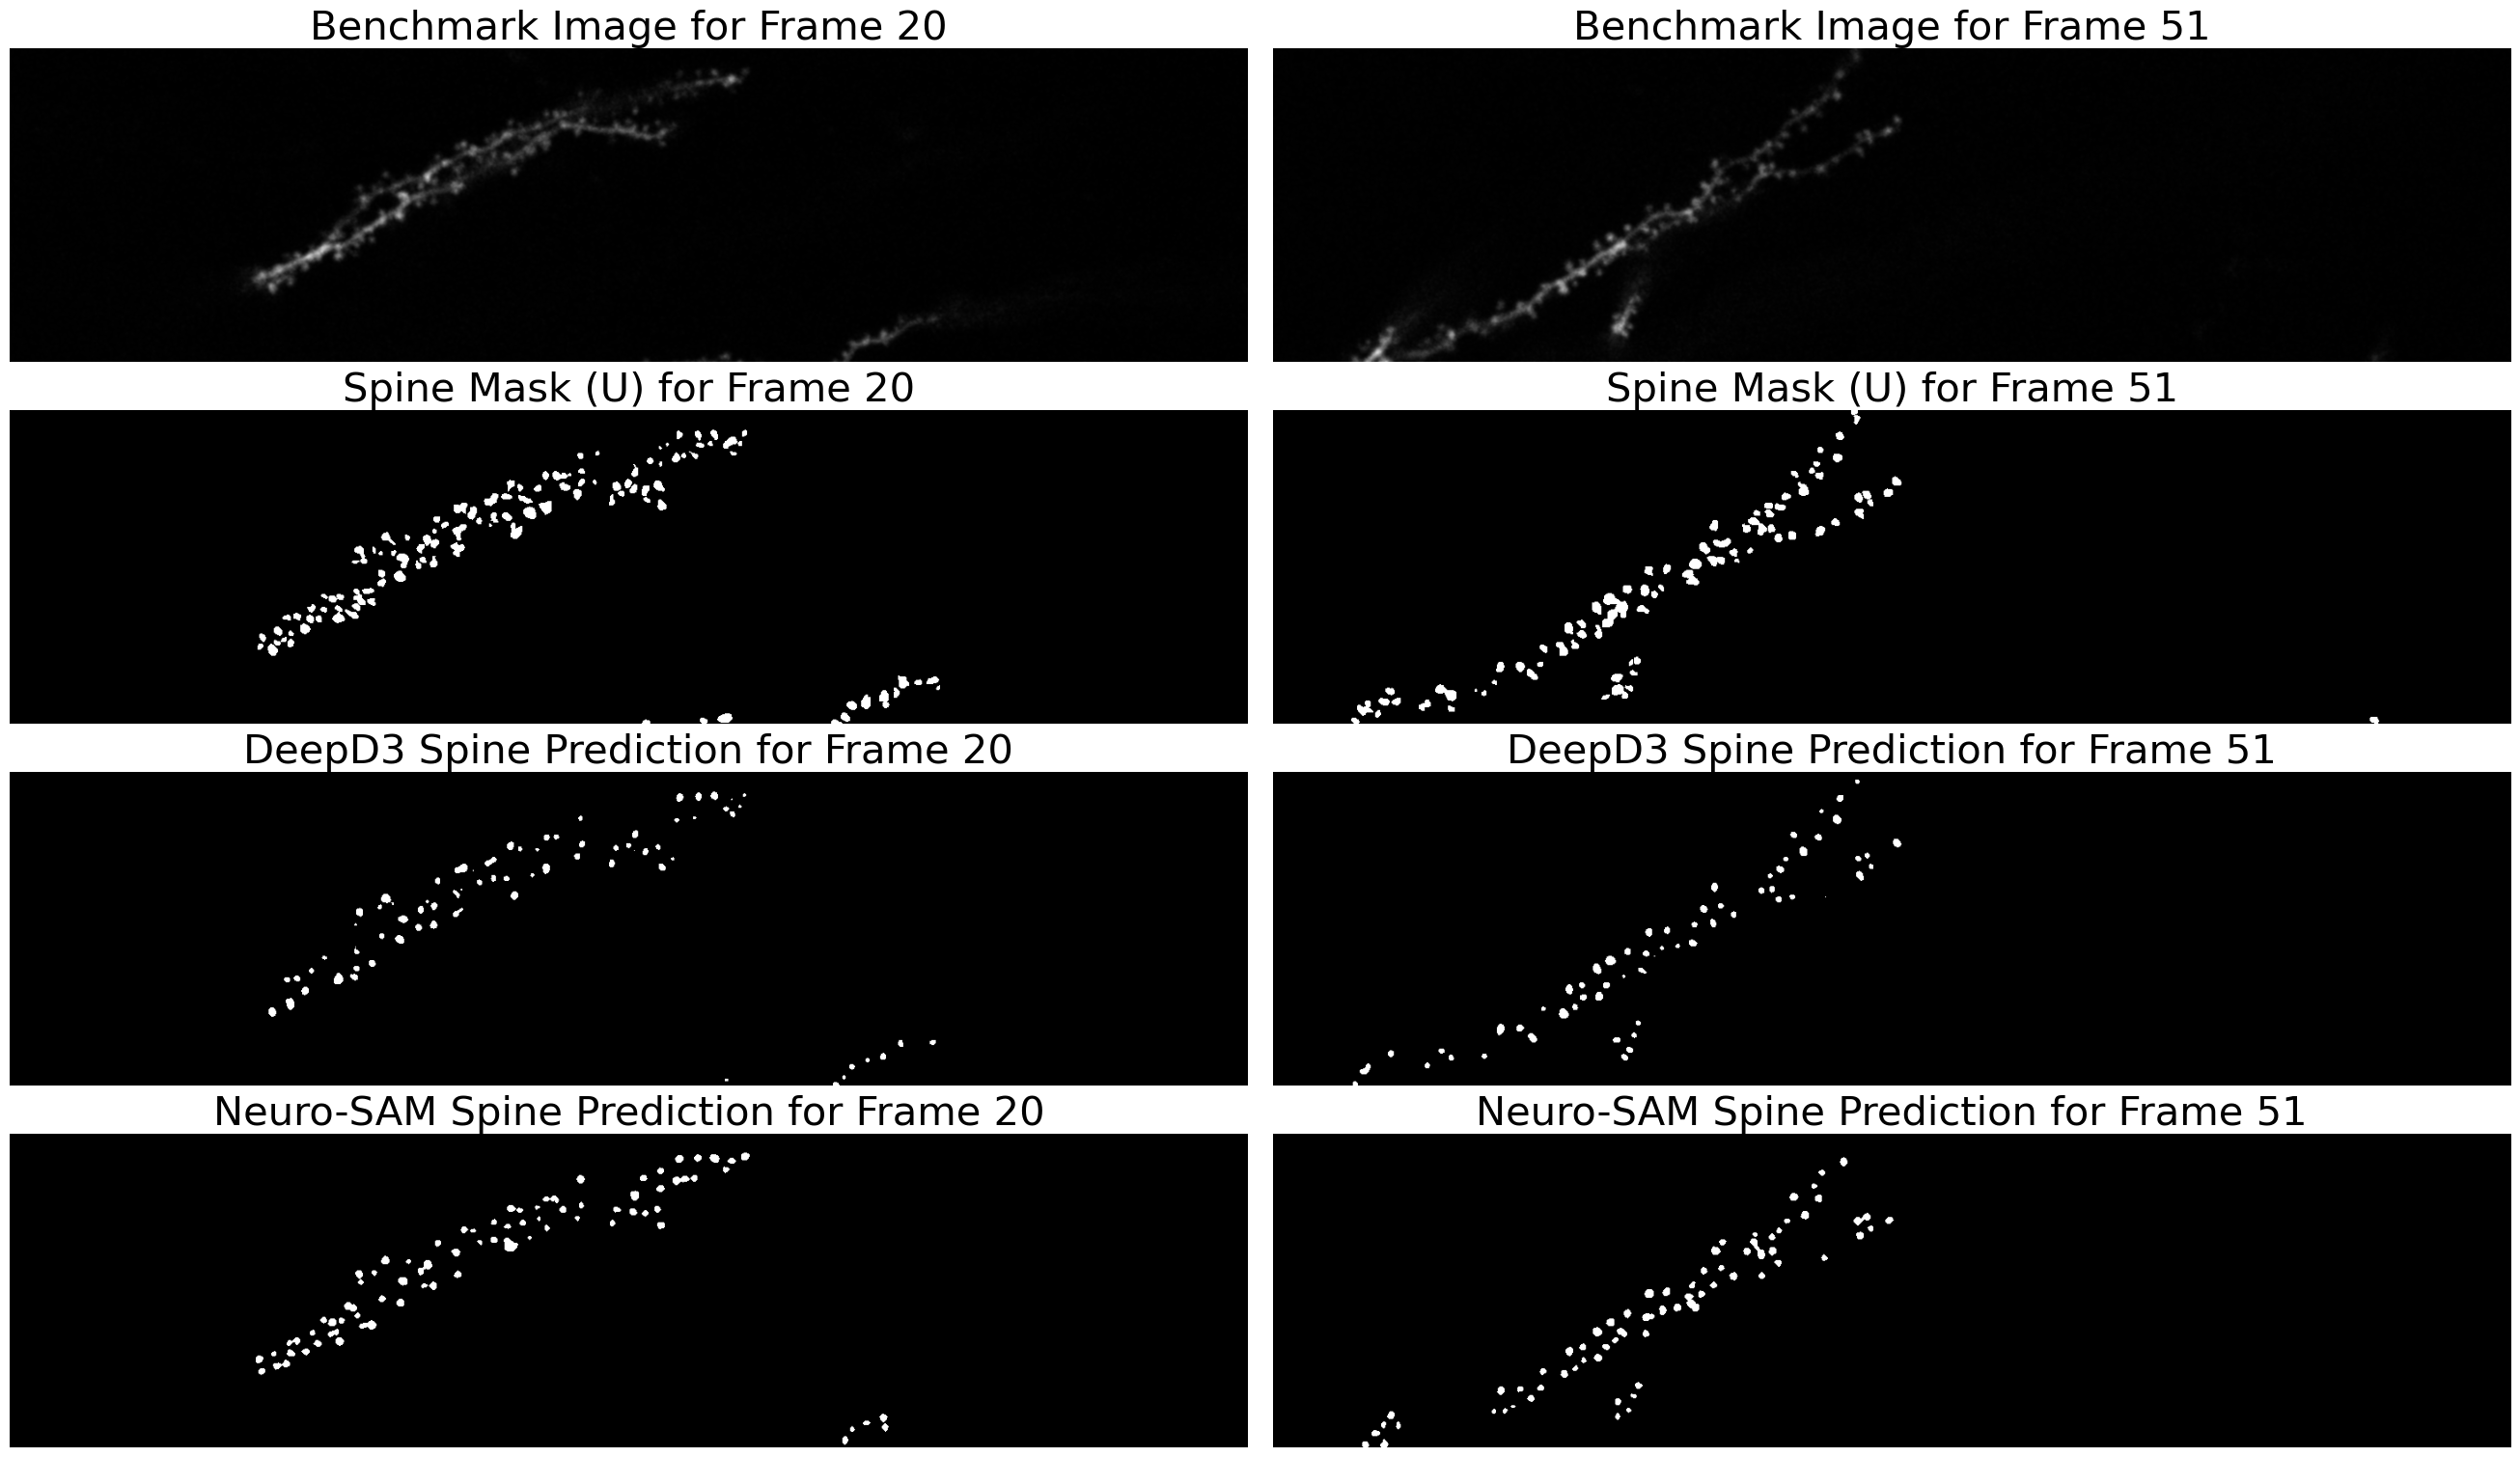
\includegraphics[width=0.95\textwidth]{figures/42_spine_seg_per_frame.png}
\captionof{figure}{Frame-wise segmentation results for spines on two different volumes. Top to bottom: raw benchmark image, ground truth annotation (rater U), \gls{DeepD3} prediction, and Neuro-\gls{SAM} prediction. Neuro-\gls{SAM} maintains more complete and consistent spine segmentation across frames. Scale: $0.94\,\mu\text{m}/\text{px}$}
\label{fig:spine_seg_per_frame}
\end{center}

\begin{center}
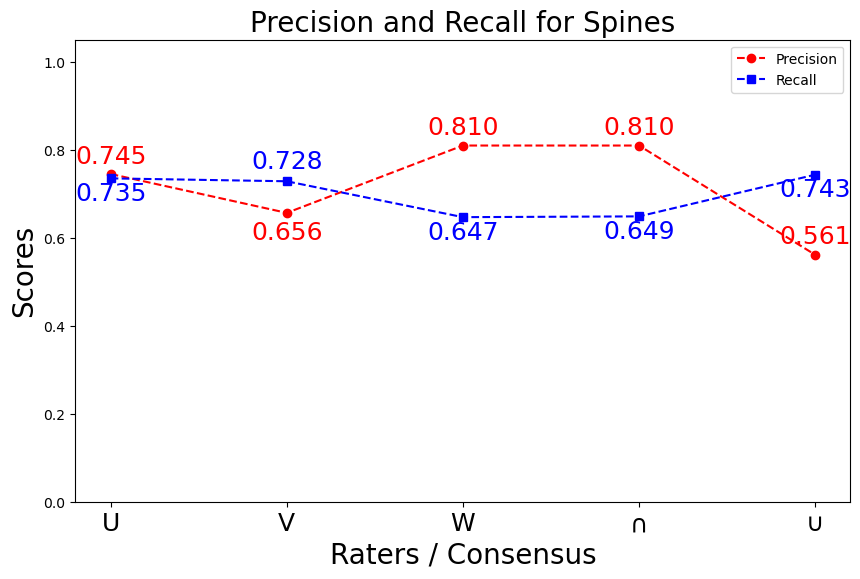
\includegraphics[width=0.8\textwidth]{figures/43_spine_precision_recall.png}
\captionof{figure}{Precision and recall scores for spine segmentation across individual raters and the consensus. Neuro-\gls{SAM} shows high precision with slightly lower recall, indicating conservative but accurate spine detection.}
\label{fig:spine_precision_recall}
\end{center}


In addition to Dice and \gls{IoU}, we analyzed the precision and recall of Neuro-\gls{SAM}’s spine predictions across all raters and the consensus (\autoref{fig:spine_precision_recall}). Neuro-\gls{SAM} exhibits high precision, particularly against raters W and $\cap$, indicating strong specificity with minimal false positives. However, recall is moderately lower, suggesting that a few spines may be missed, especially in densely clustered regions. This trade-off highlights the bias of Neuro-\gls{SAM} towards conservative segmentation, which is often desirable in scenarios where false positives can impede downstream analyses.

\begin{center}
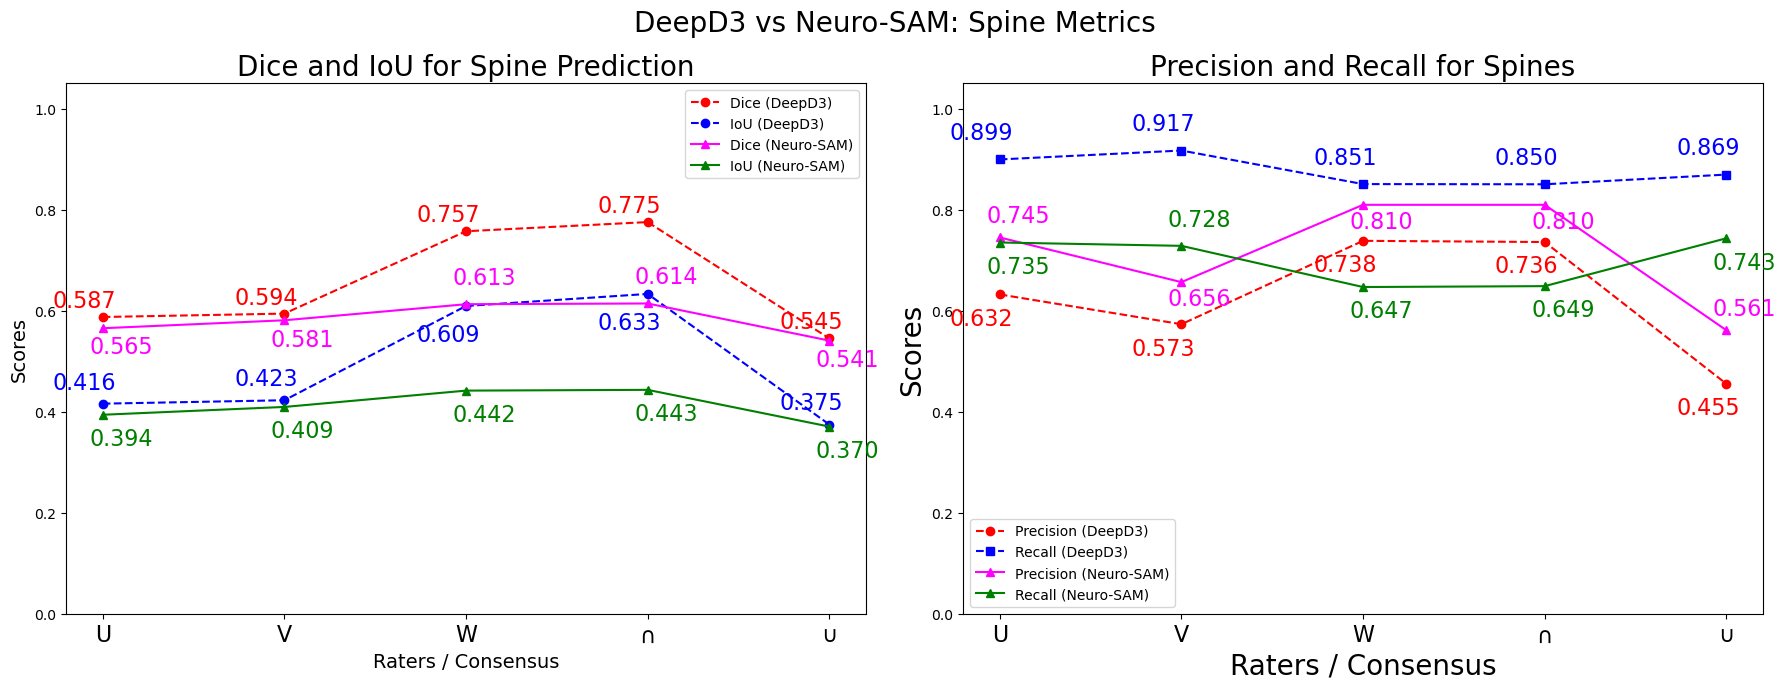
\includegraphics[width=0.98\textwidth]{figures/44_deepd3_neurosam_comparison.png}
\captionof{figure}{Comparison of \gls{DeepD3} and Neuro-\gls{SAM} on Spine Segmentation Metrics. Neuro-\gls{SAM} achieves higher precision with balanced Dice and \gls{IoU} scores, while \gls{DeepD3} demonstrates higher recall, indicating a tendency toward over-segmentation.}
\label{fig:deepd3_neurosam_comparison}
\end{center}

To further contextualize the performance of Neuro-\gls{SAM}, we conducted a head-to-head comparison with \gls{DeepD3} across Dice, \gls{IoU}, Precision, and Recall metrics. As shown in \autoref{fig:deepd3_neurosam_comparison}, \gls{DeepD3} exhibits higher recall values across all raters, suggesting that it captures more spines. In contrast, Neuro-\gls{SAM} maintains a more balanced trade-off, showing consistently higher precision while preserving reasonable recall. This conservative segmentation strategy, informed by dendrite-aware prompting and high-resolution fine-tuning, results in fewer false detections and better anatomical alignment. In addition, the Dice and \gls{IoU} scores remain comparable between both methods, underscoring the robustness and efficiency of Neuro-\gls{SAM} in generating high-quality spine masks even under noisy or ambiguous imaging conditions.

Together, these results demonstrate that Neuro-\gls{SAM} effectively extends its path-based spatial awareness to high-precision spine segmentation. While inter-rater variability and dense spatial arrangements present inherent challenges, Neuro-\gls{SAM} maintains coherent predictions, underscoring its potential as a scalable and annotation-efficient tool for fine-grained structural analysis in neuroscience.

\subsection{Generalization across other datasets}
To evaluate the robustness and adaptability of Neuro-\gls{SAM} beyond the benchmark dataset, we tested its performance on additional dendritic imaging datasets with varying signal-to-noise ratios, staining techniques, and imaging conditions. These datasets were never seen during training and were selected to challenge the model’s ability to generalize to unseen morphological patterns and contrast variations. In all cases, the full Neuro-\gls{SAM} pipeline was applied without re-training or fine-tuning. The goal of this evaluation is to assess whether our path-conditioned prompting and modular design generalize well to diverse settings while maintaining structural fidelity.

\begin{center}
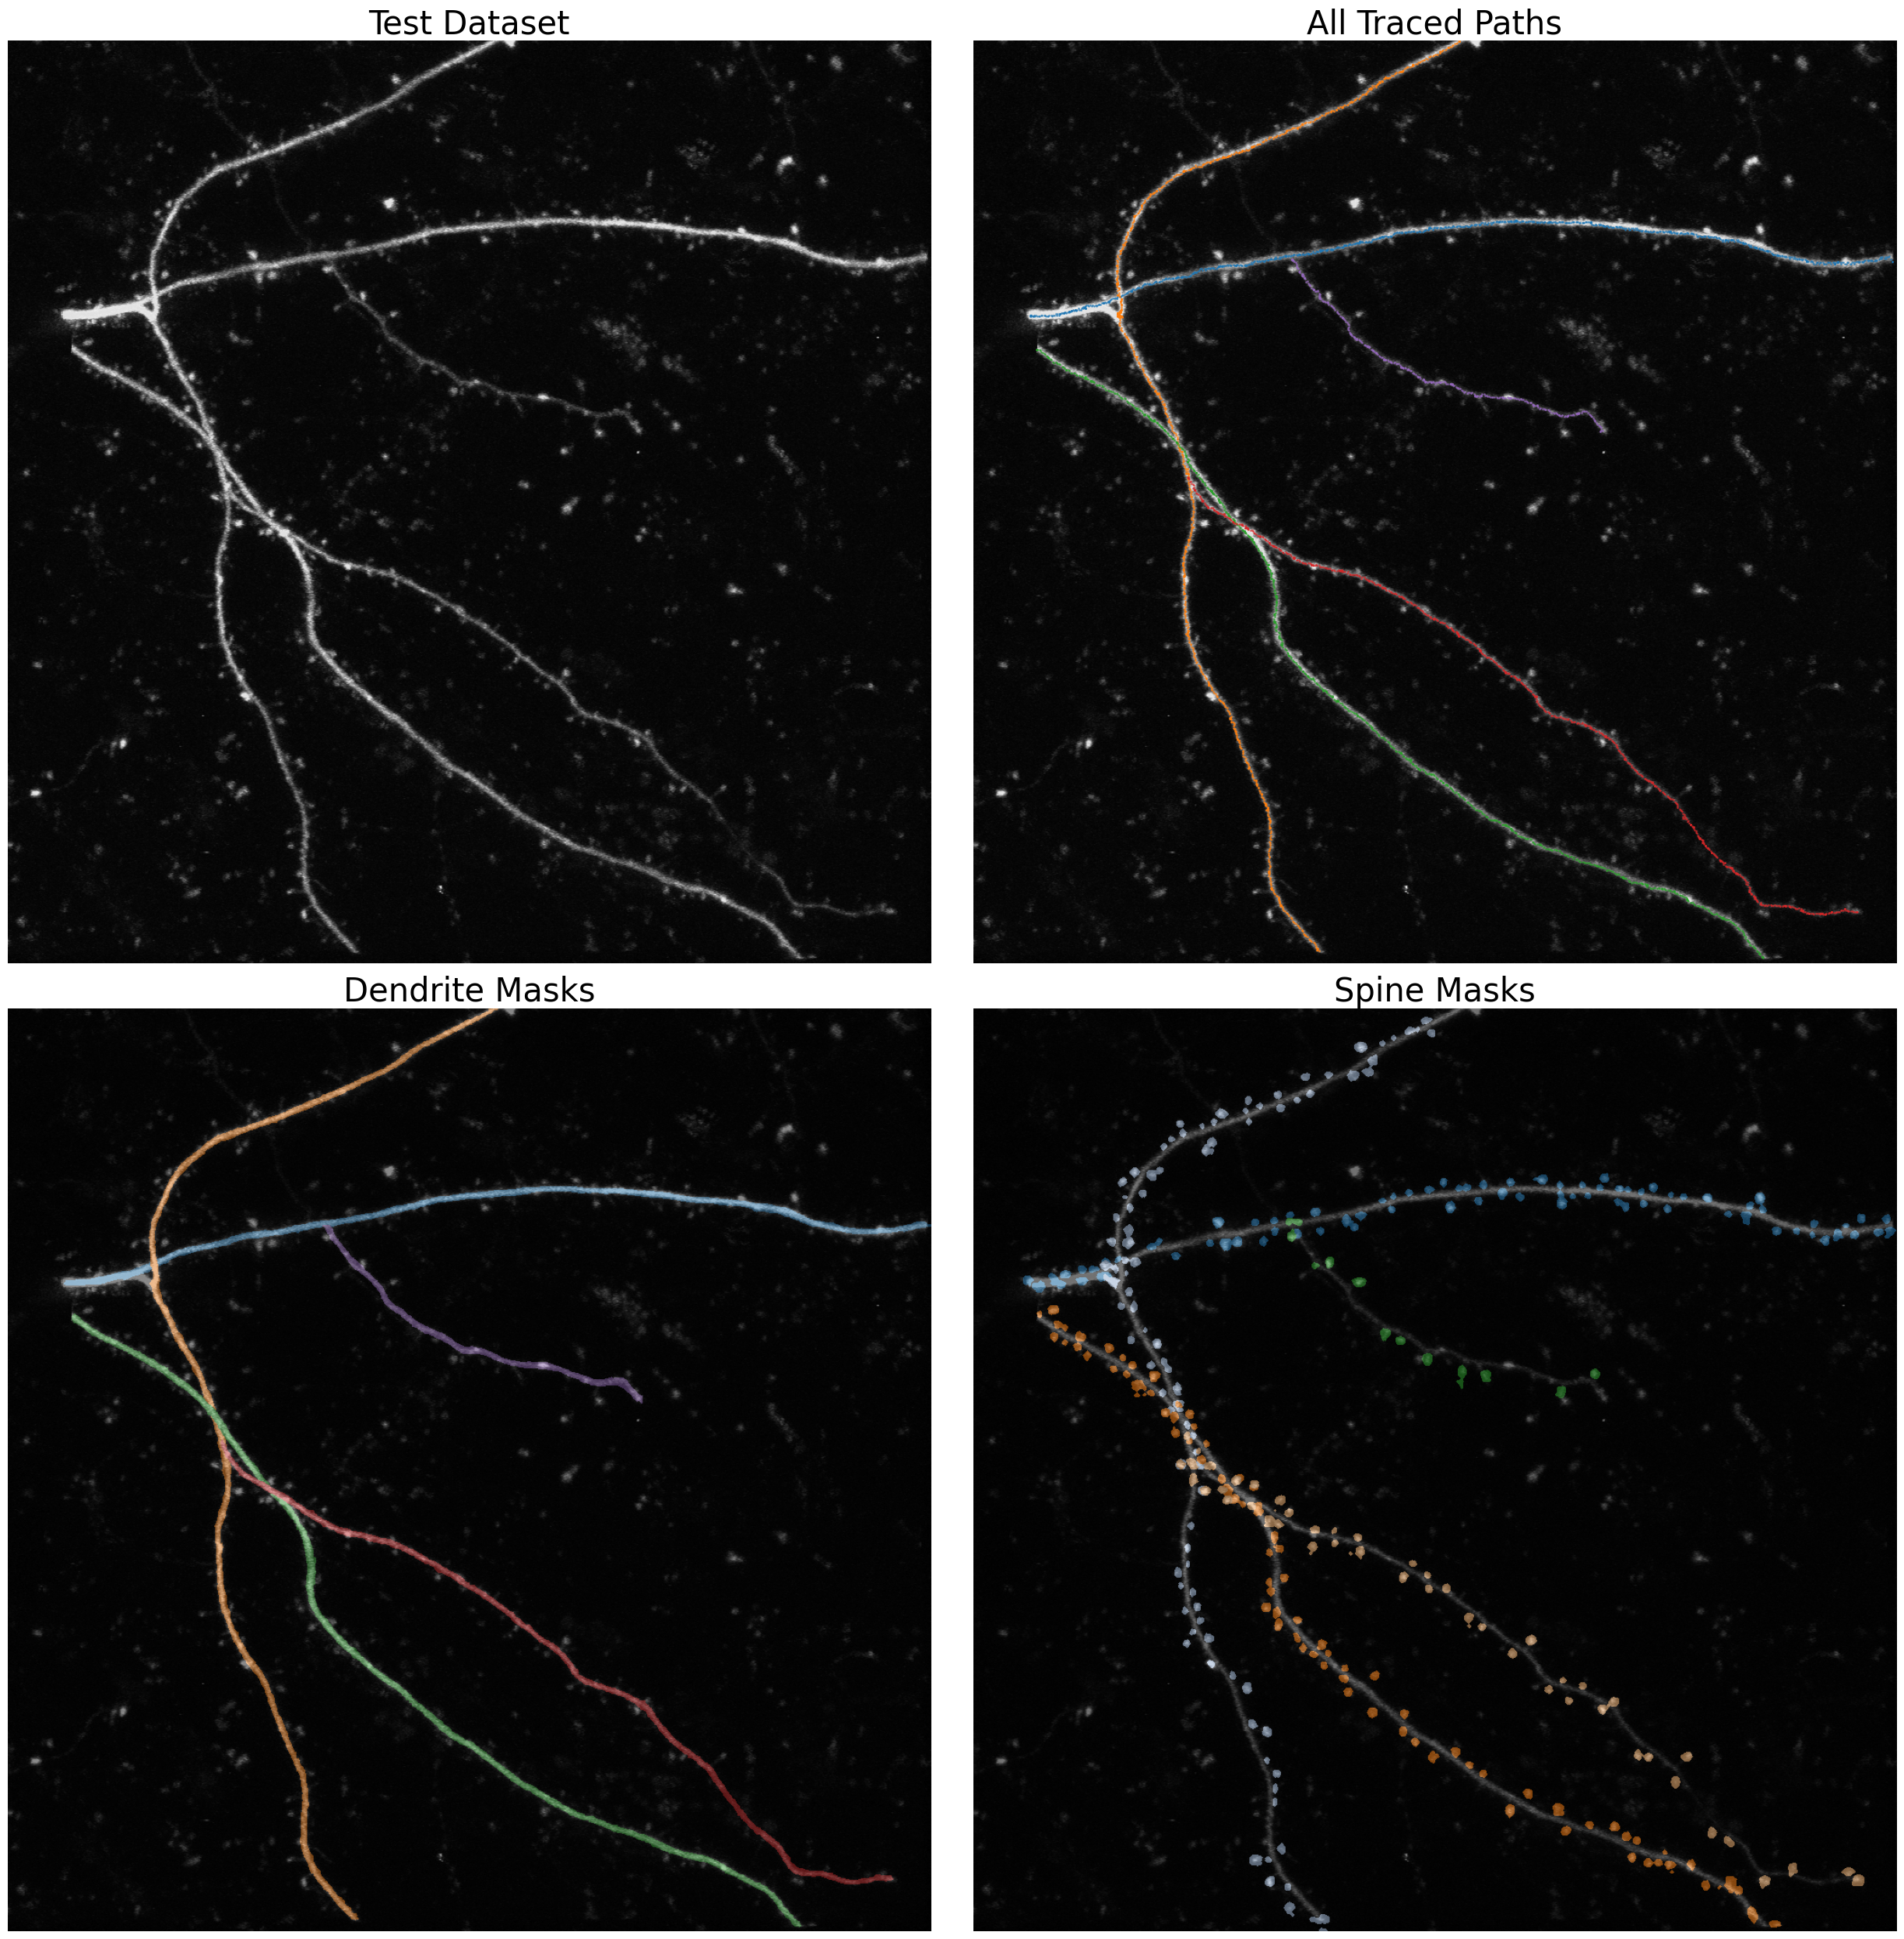
\includegraphics[width=0.95\textwidth]{figures/46_generalization_stack1.png}
\captionof{figure}{Robust results of Neuro-\gls{SAM}. The model successfully traces dendritic paths (top-right), segments dendrite shafts (bottom-left), and identifies individual spines (bottom-right) despite visual differences from the benchmark dataset. Scale: $1\,\mu\text{m}/\text{px}$}
\label{fig:generalization_stack1}
\end{center}

As illustrated in \autoref{fig:generalization_stack1}, Neuro-\gls{SAM} pipeline was also applied on this dataset. The model was able to robustly trace complex dendritic structures and generate precise, continuous masks even in morphologically and visually distinct regions. In particular, spine segmentation also remained consistent, with clear spatial alignment along the traced dendrites. These results highlight the adaptability of the pipeline to new domains, underscoring its utility in low-annotation or cross-laboratory settings.

\begin{center}
\includegraphics[width=0.8\textwidth]{figures/47_generalization_stack2.png}
\captionof{figure}{Generalization performance of Neuro-\gls{SAM} on a morphologically diverse dataset. Despite noise and complex spine shapes, the model accurately segments the dendrite shaft and detects the majority of spines along its path Scale: $1\,\mu\text{m}/\text{px}$}
\label{fig:generalization_stack2}
\end{center}

In a second generalization test, Neuro-\gls{SAM} was evaluated on a dataset with highly variable spine morphology and lower signal-to-noise ratio. As shown in \autoref{fig:generalization_stack2}, the dendrite was successfully traced and segmented with strong continuity, even across subtle changes in thickness and contrast. Spine segmentation was largely successful, capturing most spines along the shaft. However, in denser regions or where the spines were faint or elongated, the model occasionally missed or under-segmented structures. These results highlight that while Neuro-\gls{SAM} generalizes robustly, performance can be further strengthened by incorporating more morphologically diverse training samples or refining prompt adaptation strategies for challenging conditions.

\begin{center}  
\includegraphics[width=0.98\textwidth]{figures/48_generalization_stack3.png}  
\captionof{figure}{Generalization of Neuro-\gls{SAM} on a full-neuron dataset. Left: raw test dataset. Middle: traced dendritic paths. Right: dendrite segmentation masks. Spine detection was not performed due to very few visible spines. Scale: $1\,\mu\text{m}/\text{px}$}  
\label{fig:generalization_stack3}  
\end{center}  

As a final generalization test, Neuro-\gls{SAM} was applied to a dataset containing a complete neuron with extensive arborization (\autoref{fig:generalization_stack3}). Despite the increased structural complexity and large number of intersecting branches, the model reliably traced all dendritic paths from the soma and generated coherent segmentation masks for each shaft. Since this dataset contained very few visible spines, spine detection and segmentation were not performed. Nevertheless, the results confirm that Neuro-\gls{SAM} can maintain structural fidelity at whole-cell scale, effectively capturing both global morphology and fine local detail. This experiment underscores the framework’s adaptability for large-scale reconstructions, positioning it as a practical tool for comprehensive neuroanatomical mapping.


        \chapter{Discussion}

This chapter reflects on the strengths and limitations of Neuro-\gls{SAM}, placing its results in context and outlining concrete directions for future research. While the system demonstrates strong performance across tasks and datasets, several challenges remain that require further exploration and refinement.

\section{Limitations}

Despite its overall effectiveness, Neuro-\gls{SAM} presents several limitations that highlight directions for future improvement. First, while the path tracing module is interactive and efficient, it still depends on user-specified start, end, and optional waypoint inputs. Although minimal, this manual dependency limits full automation in large-scale reconstructions.

Second, the segmentation module lacks robust use of negative prompts, which constrains the model’s ability to suppress adjacent structures or competing regions. This is particularly relevant in dendrite segmentation where overlapping signals could be actively excluded using such prompts, but currently are not. Similarly, in the spine segmentation module, no negative prompting is used at all, leading to occasional false positives in background regions or over-segmentation of spine clusters.

Additionally, the spine detection module, while effective in most cases, employs a linear blob-finding approach that lacks the nonlinear decision boundaries typically offered by learning-based classifiers. This limits its capacity to differentiate between fine spines and noise in low signal-to-noise contexts. Errors in the spine segmentation module are especially evident in cases of elongated spines, fused spine necks, or ambiguous morphological boundaries, where the model may either miss a structure entirely or merge multiple spines into one. These limitations suggest the need for richer prompt engineering, advanced instance refinement, and incorporation of better models for enhanced structural accuracy.


\section{Future Work}

Several future directions can further enhance the capabilities of Neuro-\gls{SAM}. First, the path tracing module could be extended into a fully automated system by incorporating dynamic exploration strategies or learning-based path proposal networks. Such an approach could reduce the need for manual input and improve consistency across long or branching dendritic structures. Integrating active correction during tracing could also enable real-time quality control and refinement.

For the segmentation modules, future iterations may leverage the full 3D capabilities of \gls{SAMv2} during both training and inference. Currently, segmentation is performed on 2D slices with patch-level overlap; using native 3D context would allow better spatial continuity and robustness, especially around curved dendrites and spine necks. Similarly, incorporating well-structured negative prompts, especially in spine segmentation, could greatly reduce false positives and improve precision in densely labeled regions.

In terms of spine detection, moving beyond dual-view spine exploration to a more expressive, learning-based approach could offer better separation between true spines and background noise. Graph-based reasoning, shape-aware classification, or small CNN classifiers trained on frontal and tubular views could provide the nonlinearity and morphological sensitivity needed for reliable detection across diverse imaging conditions.

Lastly, while Neuro-\gls{SAM} generalizes well to multiple test datasets, further improvements could be achieved by fine-tuning the model across different microscopy modalities, staining protocols, and voxel resolutions. This would not only improve generalization but also make Neuro-\gls{SAM} deployable across a wider range of neuroscience labs and imaging platforms.
        \chapter{Conclusion}

This thesis introduced {Neuro-\gls{SAM}, a modular and interactive segmentation framework designed to address the challenges of dendrite and dendritic spine analysis in high-resolution 3D microscopy volumes. In contrast to earlier models that either relied on conventional \gls{CNN} architectures or generalized foundation models with minimal adaptation, Neuro-\gls{SAM} was purpose-built to handle the structural complexity, scale, and variability inherent to neural data. It blends several components to produce a robust and user friendly tool for segmentation of dendrites and dendritic spines. 

The path tracing module builds upon and improves the brightest-path-lib algorithm by incorporating waypoints, enabling interactive, reliable path reconstruction through densely packed dendritic fields. These paths then act as prompts for guiding the segmentation model, providing localized context through spatially sampled patches and precisely placed prompts. The dendrite segmentation module leverages a fine-tuned version of \gls{SAMv2} adapted with custom prompt strategies to generate accurate and continuous masks even in low-contrast or curved regions. Similarly, the spine segmentation module uses spatial prompts for segmentation, achieving high precision with minimal false positives.

Extensive quantitative evaluations show that Neuro-\gls{SAM} mostly outperforms \gls{SAM}, \gls{SAM}+\gls{LoRA}, and \gls{DeepD3} across both dendrite and spine segmentation tasks. It achieves high Dice and IoU scores across all expert raters and consensus masks and maintains good precision-recall tradeoffs. In qualitative comparisons, Neuro-\gls{SAM} produces cleaner, more interpretable masks with stronger alignment to human annotations, even in difficult conditions such as overlapping dendrites, dense spine clusters, and imaging noise. Furthermore, generalization experiments across multiple unseen datasets demonstrate the robustness of the pipeline, underscoring the effectiveness of its prompt-aware modular design. 

In summary, Neuro-\gls{SAM} demonstrates a robust, path-aware framework for detailed neural analysis, combining efficient path tracing, high-fidelity dendrite segmentation, and fine-grained spine segmentation. Through extensive quantitative and qualitative evaluations, in some cases it outperforms prior models across benchmark annotations and generalizes effectively to unseen datasets with diverse imaging characteristics. Its modular architecture, human-in-the-loop flexibility, and minimal reliance on dense annotations position it as a scalable solution for large-scale, interactive neuroanatomical mapping. These results not only validate the design of Neuro-\gls{SAM} but also establish its practical relevance for downstream neuroscience applications.

    \end{content}
    
    \pagenumbering{Roman}
    \setcounter{page}{\numexpr\value{savepage}}

    % References
    \references{}
    % \printbibliography
    
    % Appendix
     \begin{appendix}
        % In the appendices, use \section{} instead of \chapter{}
         \section{Training and Validation Graphs}
\label{sec:training_validation_plots}
The following graphs show the training and validation curves of the models used in this work. They offer a quick view of convergence and stability during fine-tuning without going into detailed discussion.

\subsection{Segment Anything Model (SAM)}
\label{sec:sam_plots}

\autoref{fig:samv1_training_validation} shows the training and validation plots for SAM. The Dice score and IoU improve steadily during training, yet they plateau at modest levels. This indicates that SAM struggles to capture fine morphological details of dendrites, reflecting its limited suitability for the task compared to more advanced variants.

\begin{center}
\includegraphics[width=0.8\textwidth]{figures/48_samv1_metrics.png}
\captionof{figure}{Training and Validation Dice and IOU for SAM fine-tuning.}
\label{fig:samv1_training_validation}
\end{center}

In \autoref{fig:samv1_losses}, training and validation losses show a gradual downward trend, but the relatively high values across epochs highlight SAM’s difficulty in effectively minimizing reconstruction error. The gap between training and validation further suggests limited generalization.

\begin{center}
\includegraphics[width=0.8\textwidth]{figures/49_samv1_loss.png}
\captionof{figure}{Training and validation loss curves showing convergence across epochs.}
\label{fig:samv1_losses}
\end{center}


\subsection{SAM + Low Rank Adaptation}
\label{sec:sam_lora_plots}

The Dice and IoU metrics (\autoref{fig:sam_lora_training_validation}) rise quickly in early epochs but stagnate at modest levels. Validation performance consistently lags training, indicating that LoRA adds little benefit over baseline SAM for this task.

\begin{center}
\includegraphics[width=0.8\textwidth]{figures/51_sam_lora_metrics.png}
\captionof{figure}{Training and Validation Dice and IOU for SAM fine-tuning.}
\label{fig:sam_lora_training_validation}
\end{center}


SAM+LoRA shows an initial drop in loss, but convergence is unstable at relatively high values (\autoref{fig:sam_lora_losses}). The noisy validation curve suggests weak generalization and poor stability during training.
\begin{center}
\includegraphics[width=0.8\textwidth]{figures/50_sam_lora_loss.png}
\captionof{figure}{Training and Validation Dice and IOU for SAM fine-tuning.}
\label{fig:sam_lora_losses}
\end{center}


\subsection{Segment Anything Model 2}
\label{sec:sam2_plots}

The following are the training and validation metrics for the Segment Anything Model 2, a key part of the \textbf{Neuro-SAM} pipeline. Since we trained the model on two different datasets, dendrites and dendritic spine; we will analyze their fine-tuning metrics separately. 

\paragraph{SAMv2 Dendrite Fine-Tuning}

The Dice score and IoU rapidly increase and stabilize at substantially higher values than earlier variants. Validation closely tracks training, showing reduced overfitting and improved robustness. These results highlight SAMv2’s superior capacity for capturing dendrite morphology.


\begin{center}
\includegraphics[width=0.8\textwidth]{figures/52_samv2_dendrites_metrics.png}
\captionof{figure}{Training and validation Dice score and IoU for SAMv2, indicating strong improvements and stable performance.}
\label{fig:samv2_dendrite_training_validation}
\end{center}

The SAMv2 loss curves demonstrate clear and stable convergence, with both training and validation losses consistently decreasing to low values. Unlike SAM and SAM+LoRA, the fluctuations remain minimal, reflecting better optimization and stronger generalization.

\begin{center}
\includegraphics[width=0.8\textwidth]{figures/53_samv2_dendrites_loss.png}
\captionof{figure}{Training and validation loss for SAMv2 fine-tuning on dendrites, showing smooth convergence with low final error.}
\label{fig:samv2_dendrite_loss}
\end{center}


\paragraph{SAMv2 Dendritic Spine Fine-Tuning}
\newline
Metrics improve quickly in early epochs, yet the Dice score and IoU plateau at modest values. Validation lags behind training, indicating persistent overfitting and weaker generalization. These results highlight the greater difficulty of spine segmentation compared to dendrites, even for SAMv2.

\begin{center}
\includegraphics[width=0.8\textwidth]{figures/54_samv2_spines_metrics.png}
\captionof{figure}{Training and validation Dice score and IoU for SAMv2 spine fine-tuning.}
\label{fig:samv2_spine_training_validation}
\end{center}

The loss curves decrease steadily but remain noisier than in dendrite fine-tuning. Validation loss does not settle smoothly, suggesting that SAMv2 struggles with the higher variability and smaller scale of spines.

\begin{center}
\includegraphics[width=0.8\textwidth]{figures/55_samv2_spines_loss.png}
\captionof{figure}{Training and validation loss for SAMv2 spine fine-tuning.}
\label{fig:samv2_dendrite_loss}
\end{center}
     \end{appendix}


    % Declaration of authorship
    % \authorshipstatement[pagenumbering=false]
    \authorshipstatement[pagenumbering=true]
    % \authorshipstatement[pagenumbering=only]
    
    % Consent form for use of plagiarism detection software
    % Not yet required
    % \consentform[pagenumbering=false]
    % \consentform[pagenumbering=true]
    % \consentform[pagenumbering=only]
    
    % Bonus: Wordcount
    % cd %FOLDER WHERE THE .tex FILES ARE IN %
    % clear
    % texcount -total -q -col -sum *.tex
    
\end{document}